% -----------------------------------------------------------------------------
% -----------------------    Importing Packages    ---------------------
% -----------------------------------------------------------------------------
\documentclass[a4paper]{article}
\usepackage[a4paper, total={6in, 9.5in}]{geometry}
\usepackage{graphicx}
\usepackage{amsmath}
\usepackage{wrapfig}
\usepackage{amssymb}
\usepackage{graphicx}
\usepackage{mathtools}
\usepackage{hyperref}
\usepackage[dvipsnames]{xcolor}
\usepackage{setspace}
\usepackage{enumitem} 
\numberwithin{equation}{section}
\usepackage{hyperref}
\usepackage{graphicx}
\usepackage{gensymb}
\usepackage[parfill]{parskip}
\usepackage{letltxmacro}
\usepackage{lingmacros}
\usepackage{tree-dvips}
\usepackage{pythonhighlight}
\usepackage{graphicx}
\usepackage{caption}
\usepackage{subcaption}
\usepackage[export]{adjustbox}
\usepackage{xcolor}
\usepackage [english]{babel}
\usepackage{algorithm}
\usepackage{fancyhdr}
\usepackage{algpseudocode} 
\usepackage{algpseudocode}

% -----------------------------------------------------------------------------
% -----------------------            Set-Up                ---------------------
% -----------------------------------------------------------------------------

% Hyperlink colour set up 
% If you *don't* want to change the colours of your hyperlinks, comment the below section. If you do, you can keep the below colours or change as you wish. NOTE: when you first typeset, sometimes LaTeX doesn't show the contents. Just typeset again and it should come up :) 
\hypersetup{
    colorlinks,
    linkcolor={red!50!black},
    citecolor={blue!50!black},
    urlcolor={blue!80!black}
}

% Page set up - header and footer 
\pagestyle{fancy}
\fancyhf{}
\rhead{\emph{Ellie Sleightholm}} % Input your name here 
\lhead{\emph{Wave Attractors in Rotating and Stratified Fluids}} % Input your title here 
\rfoot{Page \thepage} % Inputting the page number 

% Changing the square root so that it has a little tail at the end so you can clearly see where the square root ends 
\LetLtxMacro{\oldsqrt}{\sqrt}
\renewcommand{\sqrt}[1][\hphantom{3}]{%
  \def\DHLindex{#1}\mathpalette\DHLhksqrt}
\def\DHLhksqrt#1#2{%
  \setbox0=\hbox{$#1\oldsqrt[\DHLindex]{#2\,}$}\dimen0=\ht0
  \advance\dimen0-0.2\ht0
  \setbox2=\hbox{\vrule height\ht0 depth -\dimen0}%
  {\box0\lower0.4pt\box2}}
  
% Changing set up for absolute calculations
% Swap the definition of \abs* and \norm*, so that \abs
% and \norm resizes the size of the brackets, and the 
% starred version does not.
\DeclarePairedDelimiter\abs{\lvert}{\rvert}%
\DeclarePairedDelimiter\norm{\lVert}{\rVert}%

\makeatletter
\let\oldabs\abs
\def\abs{\@ifstar{\oldabs}{\oldabs*}}

\let\oldnorm\norm
\def\norm{\@ifstar{\oldnorm}{\oldnorm*}}
\makeatother

% Other amendments 
\makeatletter
\def\BState{\State\hskip-\ALG@thistlm}
\makeatother

\makeatletter
\renewcommand{\ALG@name}{}
\makeatother

% -----------------------------------------------------------------------------
% -----------------------   Beginning Document   ---------------------
% -----------------------------------------------------------------------------
\begin{document}

% -----------------------------------------------------------------------------
% ---------------------          Title Page            ------------------------
% -----------------------------------------------------------------------------
\begin{titlepage}
 
% Input your institution logo saved as 'logo.png' and rescale as appropriate
\raggedleft

\includegraphics[scale=0.08]{Images/logo.png}\\

% Input text above title if you wish 
\vspace{5cm}
\begin{center}
\newcommand{\HRule}{\rule{\linewidth}{0.5mm}}
\textsc{\Large Part III Essay 2021-22}\\[2.0mm]
\textsc{\Large Faculty of Mathematics, DAMTP}\\[2.0mm]
\vspace{0.8cm}
	\HRule\\[0.4cm]
	% Input title of your project 
	{\huge\bfseries Wave Attractors in Rotating and Stratified Fluids}\\[0.4cm] 
	\HRule\\[1.5cm]
		\begin{minipage}{0.4\textwidth}
		\begin{flushleft}
			\large
			\textit{Author:}\\
			% Input your name here 
			\text{Eleanor Sleightholm} \\
			% Input your student ID
			\text{(student ID)}
		\end{flushleft}
	\end{minipage}
	~
	\begin{minipage}{0.4\textwidth}
		\begin{flushright}
			\large
			% Input your supervisor
			\textit{Supervisor:}\\
			\text{Professor ...} \\
			\text{ } \\
		\end{flushright}
	\end{minipage}
\mbox{}
\vfill
% Input the date
\text{April 27, 2022}

\end{center}
\end{titlepage}

% -----------------------------------------------------------------------------
% ---------------------              Abstract           ------------------------
% -----------------------------------------------------------------------------
\newpage
\thispagestyle{empty}
% The star is next to section so that the abstract is not included in the contents page. Remove the star if you'd wish to include abstract into your contents page. 
\section*{Abstract}

A central topic in the study of waves is the behaviour of internal gravity and inertial waves and, in particular, the dynamics of such waves in real world systems. Under correct specification of the domain, these waves can generate internal wave attractors (IWAs). This essay presents a review of this phenomenon in the trapezoidal domain. Due to the analogous behaviour between internal gravity and inertial wave dispersion relations, the main focus is on internal gravity waves. An understanding of two-dimensional wave attractors in the inviscid, linear regime is presented before exploring the role of viscosity and non-linearities. In particular, dissipation in the shear layers of the attractor, at the reflecting and lateral walls (surfaces along the attractor); the effect of non-linear stratifications; and the triadic resonance instability. Finally, the propagation of internal waves are extended to the three-dimensional case where reflective conditions are described and the notion of trapping is explored. The evolution of wave attractors from ray tracing predications to viscous and non-linear effects in physical and numerical experiments is illustrated.

% -----------------------------------------------------------------------------
% ---------------------    Table of Contents      ------------------------
% -----------------------------------------------------------------------------
\newpage
\thispagestyle{empty}
% Adjust sizes here where needed 
\renewcommand{\baselinestretch}{1.34}\normalsize
\tableofcontents
\renewcommand{\baselinestretch}{1.0}\normalsize

% Remove page number as already included above 
\thispagestyle{empty}

% -----------------------------------------------------------------------------
% ---------------------   Starting the Report     ------------------------
% -----------------------------------------------------------------------------
\newpage
% Start the page counting from the first page of the report
\setcounter{page}{1}

% This makes the spacing between paragraphs bigger 
\parskip = \baselineskip

% -----------------------------------------------------------------------------
% ---------------------          Introduction         ------------------------
% -----------------------------------------------------------------------------
 \section{Introduction}
Internal gravity waves and inertial waves are ubiquitous in geophysical and astrophysical systems (Pedlosky \hyperlink{ref 1}{2003}). The former propagate through stably stratified fluids using buoyancy as a restoring force and the latter propagate through rotating fluids and are restored by Coriolis forces. Owing to their applicability in real world systems, it is important to understand the fundamental aspects governing such waves. 

As with many physical processes, exploring the effects of the domain's boundaries is paramount when understanding the steady state behaviour of the system. Indeed, when internal waves reflect within a bounded domain, they can form closed orbits known as \emph{internal wave attractors} (IWAs) (Maas \& Lam \hyperlink{ref 10}{2005}). This happens when the geometry of the domain facilitates focusing reflections. Such attractors lead to energy concentration around the internal wave orbit which induces spatial patterns as observed theoretically (Ogilvie \hyperlink{ref 13}{2005}), experimentally (Maas \emph{et al.} \hyperlink{ref 11}{1997}), and numerically (Rieutord \emph{et al.} \hyperlink{ref 12}{2001}). Of course, an infinite supply of energy is unphysical and so, viscous and non-linear effects take hold.

Although there is no evidence of wave attractors observed in nature so far, a substantial proportion of the literature considers wave attractors in closed and geometrically well-controlled domains. The fascination behind wave attractors was initiated by Maas \& Lam (\hyperlink{ref 17}{1995}) after they studied wave attractors theoretically and experimentally for the first time. Since then, the linear and non-linear state of wave attractors have been examined (Brouzet \emph{et al.} \hyperlink{ref 26}{2016}; Rieutord \emph{et al.} \hyperlink{ref 12}{2001}; Ogilvie \hyperlink{ref 13}{2005}). Indeed, any initial energy injected into the system will become focused around the attractor and so one expects instability if this energy becomes too large.

Section (\hyperref[sec:2]{2}) introduces internal waves in stratified and rotating fluids where the properties of such waves are established. The reflective properties of these waves are then considered. Section (\hyperref[sec:3]{3}) presents 2D IWAs in a trapezoidal domain. The wave equation governing the behaviour of internal waves is established with particular emphasis on it's ill-posedness. Techniques used to overcome this are then presented. Certain conditions are then derived for the existence of IWAs. Section (\hyperref[sec:4]{4}) introduces the idea of viscous attenuation and how the equilibrium thickness of the IWA varies according to parameters of the problem. Section (\hyperref[sec:5]{5}) illustrates the notion of non-linear stratification and its effect on the structure of the internal wave beam. Two different stratification profiles are considered and observed. Section (\hyperref[sec:6]{6}) presents the effect of triadic resonant instability where the injected energy becomes too large and results in instabilities. Finally, Section (\hyperref[sec:7]{7}) extends the previous findings to the 3D case where inviscid internal waves are considered in a 3D trapezoidal domain. Conditions on reflective properties and the notion of the trapping effect are considered. Attention is then drawn to future work in the area of IWAs.

% -----------------------------------------------------------------------------
% -----------      Start Writing After Introduction     -----------------
% -----------------------------------------------------------------------------
\newpage

\section{Introduction to Internal Waves}
\label{sec:2}
Internal gravity and inertial waves are waves propagating within stably stratified and rotating fluids respectively. Stratification may result from temperature, density or concentration gradients as seen in oceans and atmospheres on Earth (Pedlosky \hyperlink{ref 1}{2003}). Rotating fluids can be seen on Earth but also in other astrophysical objects such as stars or planets (Ogilvie \& Lin \hyperlink{ref 2}{2004}). As a result, internal waves play a vital role in these systems which underpins much of the discussion in this essay. 

\subsection{Governing Equations}

Consider a rotating, incompressible and stably stratified fluid in 3D. The governing equations are given by the Navier-Stokes equations under the Boussinesq approximation (Kundu \emph{et al.} \hyperlink{ref 3}{2016}), 
% Input * if you don't want to include the equations labelling 
\begin{align*}
\begin{split}
\frac{D\mathbf{u}}{Dt} + f\mathbf{\mathbf{\hat{z}}}\times \mathbf{u} &=-\frac{1}{\rho_0} \nabla p' + \frac{\rho'}{\rho_0}\mathbf{g} + \nu \nabla^2 \mathbf{u}, \\
\nabla \cdot \mathbf{u} &= 0, \\
\frac{D\mathbf{\rho'}}{Dt} &= \kappa \nabla^2\rho,\\
\end{split}
\end{align*}
where $\mathbf{u} = (u,v,w)$ is the velocity, $\mathbf{g} = (0, 0, -g)$ is the gravitational force per unit mass, $f = 2\Omega\sin\theta$ is the Coriolis parameter. The density, $\rho$, has been decomposed into $\rho = \rho_0 + \rho'$ where $\rho_0$ is constant and $\rho'/\rho_0 \ll 1$. Then, the pressure may be split into two parts: $p_0(z)$ and $p'$ where $p_0(z)$ is in hydrostatic balance with $\rho_0$ i.e. $dp_0/dz + \rho_0g = 0$. Moreover, $\nu$ is the kinematic viscosity, $\kappa$ denotes the diffusive coefficient of the stratifying agent and $\mathbf{\hat{z}}$ is the unit vector in the vertical.

Now divide $\rho'$ into a background or reference density, $
\rho_s(z)$, and a disturbance density, $\tilde{\rho}$, such that $\rho'(x,y,z,t) = \rho_s(z) + \tilde{\rho}(x,y,z,t)$. By linearising about a state of rest, the equations reduce to, 
\begin{align}\label{eq:2.1}
\frac{\partial\mathbf{\tilde{u}}}{\partial t} + f\mathbf{\hat{z}} \times \tilde{\mathbf{u}}&=-\frac{1}{\rho_0} \nabla \tilde{p} - \frac{\tilde{\rho} g}{\rho_0}\mathbf{\hat{z}},\\\label{eq:2.2}
\nabla \cdot \mathbf{\tilde{u}} &= 0,\\\label{eq:2.3}
\frac{g}{\rho_0}\frac{\partial \tilde{\rho}}{\partial t} &= N^2\tilde{w},
\end{align}
where viscosity and diffusion are neglected, $(\tilde{~})$ denotes disturbance quantities away from the background resting state and $N^2 = -\frac{g}{\rho_0}\frac{d\rho_s}{dz}$ is the \emph{Brunt-Väisälä} or \emph{buoyancy frequency} which measures the stability of the background density. Now, seeking plane-wave solutions such that, 
\begin{align*}
\mathbf{\tilde{u}} = \text{Re}\big[ \mathbf{\hat{u}}~ e^{(i(\mathbf{k}\cdot \boldsymbol{x} - \omega t))} \big],
\end{align*}
etc., where $\mathbf{k} = (k, l, m)$ is the spatial wavenumber and $\boldsymbol{x} = (x, y, z)$. Then, equations \eqref{eq:2.1} - \eqref{eq:2.3} reduce to, 
\begin{equation*}
\begin{aligned}
-i\omega \hat{u} - f\hat{v} = - \frac{1}{\rho_0}k\hat{p}, ~~~~~
-i\omega \hat{v} + f\hat{u} = - \frac{1}{\rho_0}l\hat{p}, ~~~~~
-i\omega \hat{w}= - \frac{1}{\rho_0}m\hat{p} + \frac{\hat{\rho}g} {\rho_0},\\
-i\omega \frac{g\hat{\rho}}{\rho_0} + N^2\hat{w} = 0, ~~~~~~~
i\mathbf{k} \cdot \mathbf{\hat{u}} = 0. ~~~~~~~~~~~~~~~~~~~~~~
\end{aligned}
\end{equation*}
Eliminating between variables, one uncovers the dispersion relation (LeBlond \& Mysak \hyperlink{ref 4}{1981}), 
\begin{align}\label{eq:2.4}
\omega^2 = \frac{N^2(k^2 + l^2) + f^2m^2}{k^2 + l^2 + m^2} = N^2\sin^2(\theta) + f^2\cos^2(\theta),
\end{align}
where $\theta$ is defined as the angle between the vertical $z$-axis and the wave vector, $\mathbf{k}$. This is the dispersion relation for gravito-inertial waves but one can easily recover the dispersion relation for purely internal gravity (inertial) waves by setting $f = 0$ ($N = 0$). 

The dispersion relation highlights a dependence on the angle of propagation of the wave and in particular, the direction of the wavevector. Parallels cans be drawn between the two types of waves by noticing that changing the boundary at which $\theta$ is measured with respect to, returns similar dispersion relations. Thus, similarities can be drawn between inertial waves and the findings in this essay which focus on internal gravity waves.

Consider the dispersion relation for internal gravity waves in the $(x,z)$ plane with $N = const.$,
\begin{align}\label{eq:2.5}
\omega = \pm N \sin \theta.
\end{align}
Note, $\theta$ is determined only by $N$ and the frequency of the waves if $\omega \leq N$ which is the range of $\omega$ considered in this essay. In the case, $\omega > N$, $\theta$ does not exist and the waves are evanescent. This dispersion relation must therefore have four couples $(\pm k, \pm m)$ which forms the classic St. Andrew's Cross pattern (Mowbray \& Rarity \hyperlink{ref 5}{1967}) as depicted in Figure \ref{fig:1}. The problem can be extended to 3D, known as the spatial case, which is explored in further detail in Section (\hyperref[sec:7]{7}).

Calculating the group velocity, one finds, 
\begin{align}\label{eq:2.6}
\mathbf{c}_g = \frac{\partial \omega}{\partial \mathbf{k}} =  \text{sign}(k) \frac{Nm}{|k|^3}(m, - k),
\end{align}
where $\text{sign}(k)$ equals $+1$ for $k > 0$ and $-1$ for $k<0$. Note that $\mathbf{c}_g \cdot \mathbf{k} = 0$ and hence, $\mathbf{c}_g \cdot \mathbf{c}_p = 0$ by the definition of $\mathbf{c}_p$. Thus, the group propagation is perpendicular to phase propagation (Mowbray \& Rarity \hyperlink{ref 5}{1967}) as depicted in Figure \ref{fig:1}. Therefore, $\theta$ represents the angle of energy propagation with respect to the horizontal. It's also worth noting that these plane waves are also exact solutions to the more general non-linear problem by noting that $\mathbf{u} \perp \mathbf{k}$ from equation \eqref{eq:2.2}.

\begin{figure}[h!]
\centering
\begin{subfigure}[t]{.5\textwidth}
  \centering
  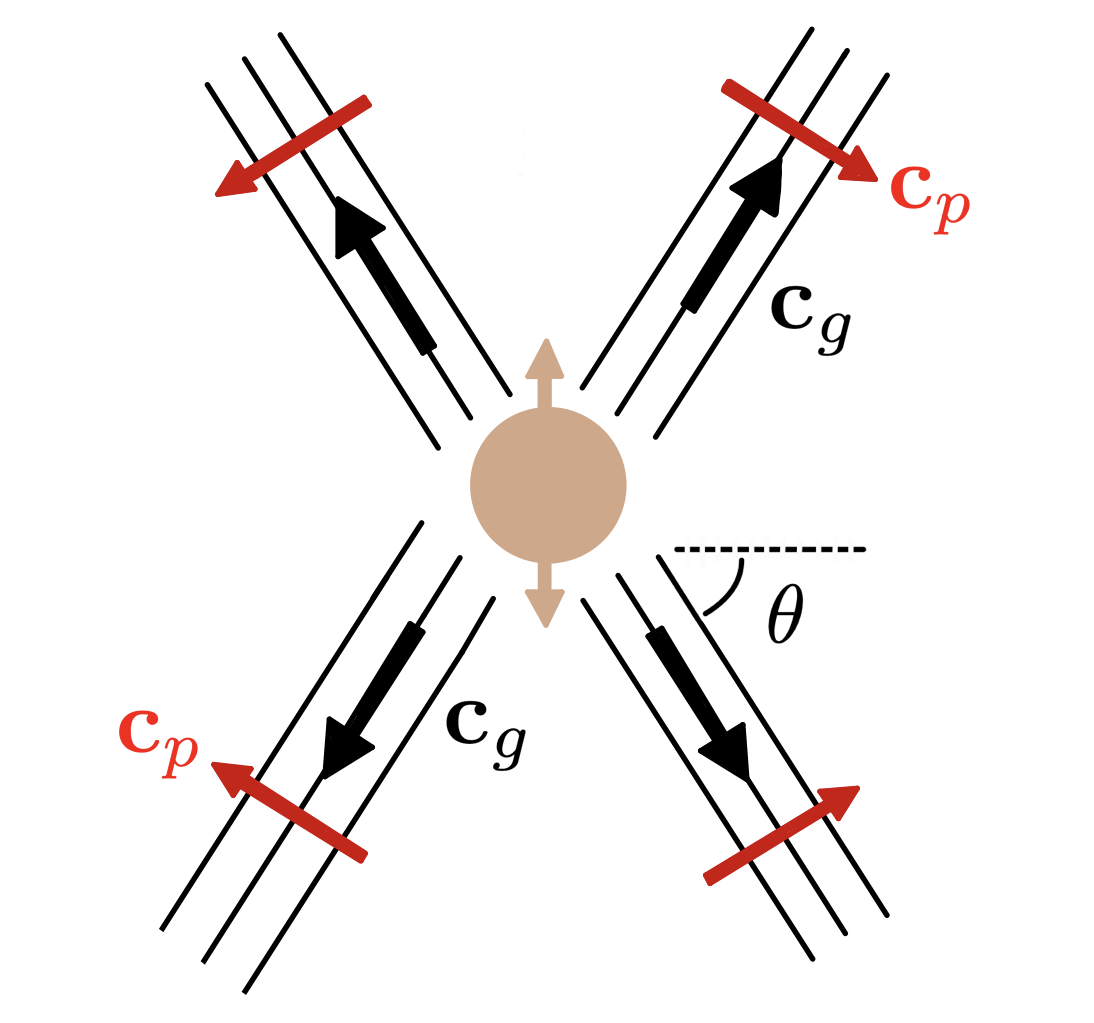
\includegraphics[width=0.6\linewidth]{Images/internal wave pic.PNG}
  \caption{Schematic diagram.}
  \label{fig:sub1}
\end{subfigure}
\begin{subfigure}[t]{.48\textwidth}
  \centering
  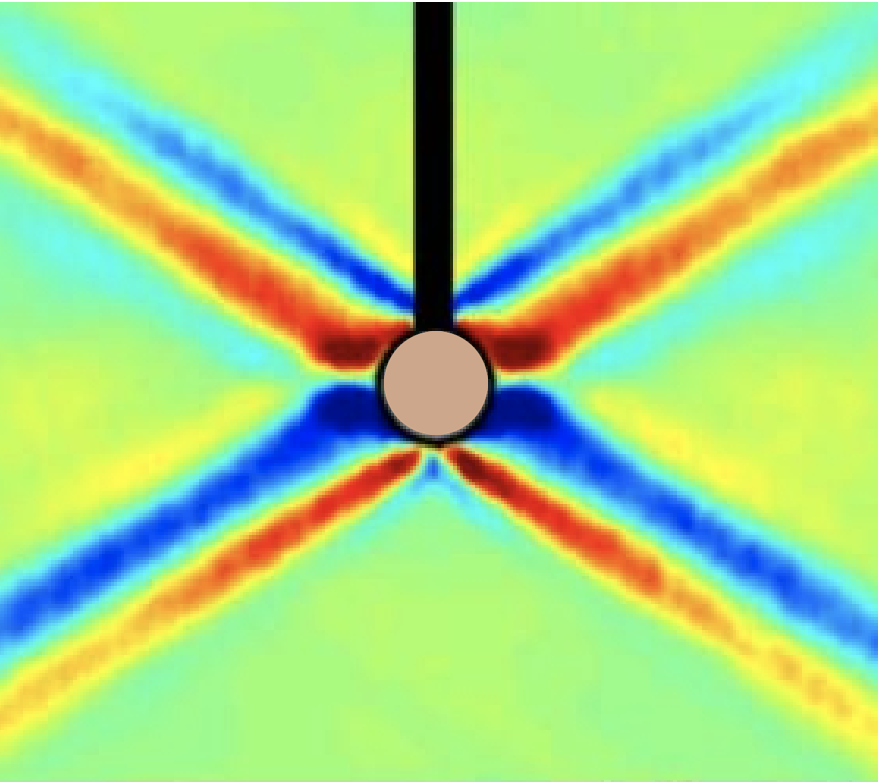
\includegraphics[width=0.64\linewidth]{Images/experiment two}
  \caption{Experiment.}
  \label{fig:sub2}
\end{subfigure}
\caption{Internal gravity waves propagating in a linearly stratified fluid. Generated by oscillating a cylinder (in beige) with frequency smaller than the buoyancy frequency. (a) A predicted visualisation with group propagation depicted by black arrows and phase propagation by red. The angle $\theta$ is defined for one beam. (b) Experimental results obtained by Gostiaux \emph{et al} (\protect\hyperlink{ref 6}{2006}). The colours depict the horizontal density gradient fields.}
\label{fig:1}
\end{figure}

\subsection{Reflection of Internal Waves}
Clearly an internal wave's angle of propagation varies as $N$, $f$ and $\omega$ vary. As a result, the reflection of these waves differ greatly when compared against standard Decartes reflection in geometric optics (Pedlosky \hyperlink{ref 1}{2003}) where the angle of incidence and reflection are conserved with respect to the normal at the point of incidence. The theory of linear internal waves was first developed by Phillips (\hyperlink{ref 7}{1966}) and holds a very specific reflective property that is fundamental to wave attractors. 

The dispersion relation \eqref{eq:2.4} contains no length scale so the width of a wave beam can be neglected and the propagation of internal waves can be described as rays. Adopting this approach, one now considers 2D internal gravity waves in the $(x, z)$ plane in an inviscid fluid with $N = const.$. Waves are initially forced with given frequency $\omega$ and propagate downwards in the positive $x$-direction towards a rigid plane boundary that is sloping up with angle $\alpha$ relative to the vertical as seen in Figure \ref{fig:2}. Following as in Pedlosky (\hyperlink{ref 1}{2003}) and Phillips (\hyperlink{ref 7}{1966}):
\begin{figure}[h!]
  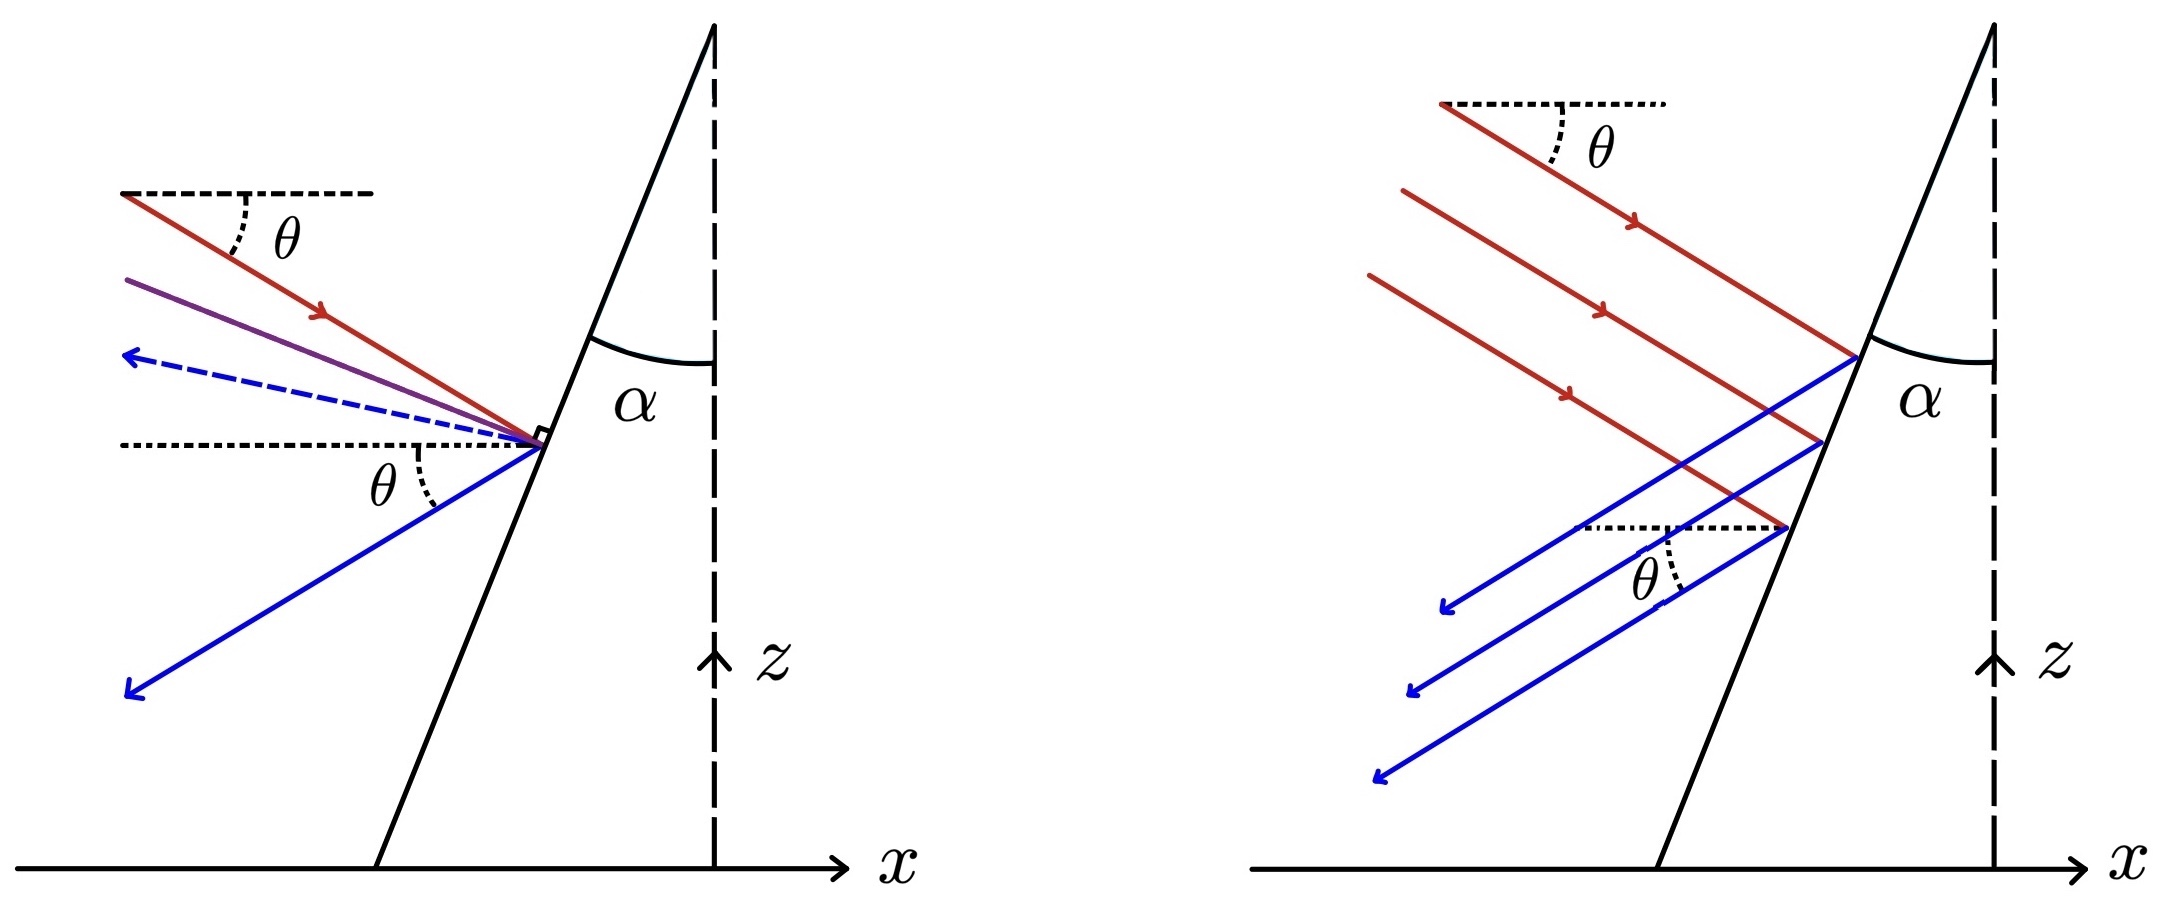
\includegraphics[scale=0.13, center]{Images/reflection.jpg}
  \caption{Reflection of an internal wave ray on a boundary inclined at $\alpha$ with the vertical. Incident (reflected) ray in red (blue). The left-hand depicts a single wave ray reflection with an optically reflected ray shown in dashed blue. The normal is in purple. The right-hand illustrates a focusing reflection where three incident waves become closer upon reflection. Based on Sibgatullin (\protect\hyperlink{ref 19}{2019}).}
  \label{fig:2}
\end{figure}\\
First, assume that the incident wave (depicted in red in Figure \ref{fig:2}) has the velocity structure, 
\begin{align*}
w_i = w_{0,i}\exp(i(k_ix+m_iz-\omega_i t)),
\end{align*}
where the subscript $i$ denotes the properties of the incident wave such that they verify the dispersion relation. For the boundary condition to match, one adds a reflected wave of similar form, 
\begin{align*}
w_r = w_{0,r}\exp(i(k_rx+m_rz-\omega_r t)).
\end{align*}
By noting that there must be no flow across the boundary and the frequency is conserved upon reflection, $\omega_i = \omega_r$, one finds that the boundary condition results in two relations, 
\begin{align}\label{eq:2.7}
w_{0,i}(\cos \alpha + \frac{m_i}{k_i}\sin\alpha) + w_{0,r}(\cos \alpha + \frac{m_r}{k_r}\sin\alpha) =&~ 0, \\ \label{2.8}
k_i + m_i\tan \alpha - k_r - m_r\tan\alpha =&~ 0.
\end{align}
Now, using the dispersion relation and noting the conservation of the frequency, it must follow that $m_r = \pm k_r\tan\theta$. Hence, by equation \eqref{2.8}, $k_i(1 + \tan\alpha\tan\theta) = k_r(1 \pm \tan\alpha\tan\theta)$. If ‘$+$' is taken then $k_i = k_r$ and $m_i = m_r$ and so the incident wave is duplicated which is inconsistent. Thus,
\begin{align*}
k_r = k_i\frac{1 + \tan\alpha\tan\theta}{1 - \tan\alpha\tan\theta} = k_i \frac{\cos(\theta - \alpha)}{\cos(\theta + \alpha)}.
\end{align*}
Thus, the ratio between the norms of the two wave vectors is, 
\begin{align}\label{eq:2.9}
\frac{k_r}{k_i} = \frac{\cos(\theta - \alpha)}{\cos(\theta + \alpha)} \equiv \gamma,
\end{align}
where $\gamma$ is the \emph{focusing parameter}. For $\gamma > 1$, the internal waves are said to be focused as illustrated in Figure \ref{fig:2} where the reflected ray is reduced by a factor of $\gamma$. For $\gamma < 1$, the internal waves become defocused. In the \emph{critical reflection} limit, $\theta + \alpha \rightarrow \frac{\pi}{2}$, $\gamma$ diverges and the wave's propagation angle becomes parallel to the sloped boundary and so, the boundary condition is not well-matched. In contrast, in the presence of horizontal or vertical walls, focusing is absent and $\gamma = 1$. 

It has been shown (Beckebanze \emph{et al.} \hyperlink{ref 8}{2018}) that for closed domains with sloping boundaries, focusing mainly dominates. The following section will illustrate such a domain where, under correct specification of $\theta$, ray trajectories will become infinitely long and after successive reflections, will evolve onto periodic orbits known as \emph{wave attractors}. Upon a focusing reflection, the energy is concentrated and one can show that equation \eqref{eq:2.9} leads to $E_r = \gamma^2 E_i$ where $E$ is the energy density (Brouzet \hyperlink{ref 9}{2016}) . Thus, if energy is supplied to a closed region at fixed frequency, the energy will be focused onto the wave attractor. In the inviscid case, the energy tends towards infinity and so, when considering real physical processes, one must consider the effects of viscosity and non-linearities that act to stop this infinite of energy. 

\section{2D Internal Wave Attractors}
\label{sec:3}
Over two decades ago, Maas \& Lam (\hyperlink{ref 10}{1995}) studied the fascinating phenomena of wave attractors for the first time theoretically. Since then, experimental attractors have been observed in laboratory experiments (Maas \emph{et al.} \hyperlink{ref 11}{1997}), visualised numerically (Rieutord \emph{et al.} \hyperlink{ref 12}{2001}) and described theoretically (Ogilvie \hyperlink{ref 13}{2005}). Before exploring such methods, it is first necessary to understand the equations governing internal wave attractors. 

\subsection{Monochromatic Wave Solutions}
By considering the incompressibility condition \eqref{eq:2.2}, a streamfunction, $\psi$ can be introduced, 
\begin{align}\label{eq:3.1}
u = -\frac{\partial\psi}{\partial z}, ~~~~ w = \frac{\partial\psi}{\partial x}.
\end{align}
One can then show that the equations of motion,  \eqref{eq:2.1} - \eqref{eq:2.3}, reduce to (Muller and Liu \hyperlink{ref 14}{2000}),
\begin{align}\label{eq:3.2}
\frac{\partial^2\psi}{\partial z^2} - \frac{N^2 - \omega^2}{\omega^2 - f^2}\frac{\partial^2\psi}{\partial x^2} = 0.
\end{align}
This spatial Poincaré equation describes the propagation of linear, inviscid, internal waves. Initially, a uniformly stratified, $N = const.$, and unforced internal wave problem will be considered; the free surface is quiescent and the fluid domain's boundary is a streamline,
\begin{align}\label{eq:3.3}
\psi = 0 ~~~ \text{on} ~~~ \partial \mathcal{D},
\end{align}
for a domain $\mathcal{D}$. To understand the nature of internal waves in this domain, a solution must be found. However, it's formally an ill-posed problem (Swart \emph{et al.} \hyperlink{ref 15}{2007}). Indeed the trivial solution $\psi \equiv 0$ holds true and in the case of a simple domain, infinitely many solutions are known to exist.  

\subsubsection*{A Simple Domain}
Consider internal waves in the absence of rotation in a rectangular domain $(x, z) \in [0,1] \times [0, l]$. Then, \eqref{eq:3.2} can be solved (Bajars \emph{et al.} \hyperlink{ref 16}{2012}) through a separation of variables. The function, 
\begin{align*}
\psi = A_{n,m}\sin(n\pi x)\sin\bigg(\frac{m \pi z}{c}\bigg),
\end{align*}
satisfies the hyperbolic equation \eqref{eq:3.2} and boundary condition \eqref{eq:3.3} provided, 
\begin{align*}
c = \sqrt{\frac{\omega^2}{N^2 - \omega^2}}~\frac{m}{n}.
\end{align*}
By transforming the integers such that $(n, m) \rightarrow (sn, sm)$ where $s \in \mathbb{R}$, the value of $c$ remains unchanged. Further, the boundary condition is satisfied for $s \in \mathbb{Z}$. Thus, there is an infinite set of solutions to the wave equation \eqref{eq:3.2} and hence, the problem is ill-posed for this domain. 

\subsection{Ray Tracing}
Ray tracing in uniform stratifications has been used to observe and predict internal wave behaviours and patterns (Maas \& Lam \hyperlink{ref 10}{2005}). Generally, the solution of the wave equation \eqref{eq:3.2} is, 
\begin{align}\label{eq:3.4}
\psi(x,z) = f(x+\lambda z) - g(x-\lambda z), ~~~~~~~ \lambda^2 = \frac{N^2 - \omega^2}{\omega^2 - f^2},
\end{align}
for arbitrary functions $f$ and $g$ with $N$ uniform (Maas \hyperlink{ref 39}{2005}). Here, $f$ is constant along characteristic lines $x+ \lambda z = const.$ and similarly, $g$ is constant along lines $x- \lambda z = const.$. Assume $f$ is known on the characteristic $x+ \lambda z = c_1$ such that $f(c_1) = f_1$. If this characteristic reaches a slope, as depicted in Figure \ref{fig:3}, then the emanating characteristic from this intersection will be $x- \lambda z = c_2$ where $g(c_2) = g_2$.
\begin{figure}[h!]
  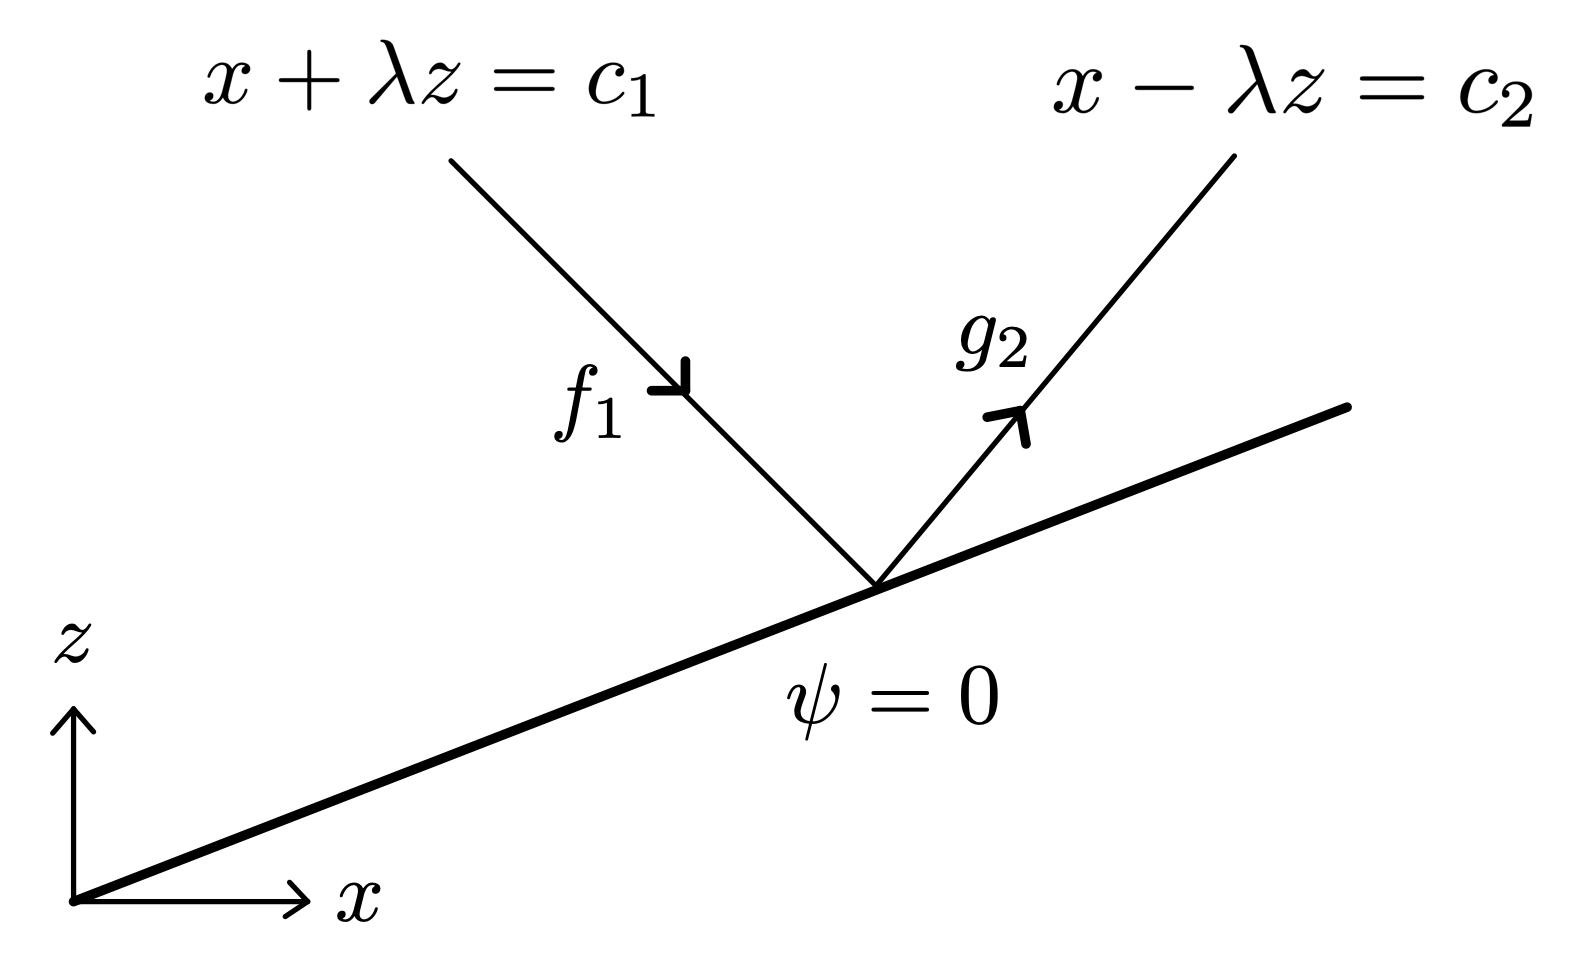
\includegraphics[scale=0.11, center]{Images/rays}
  \caption{Characteristics reflecting from a sloped boundary. Based on Maas (\protect\hyperlink{ref 39}{2005}).}
  \label{fig:3}
\end{figure} \\
For an unforced internal wave problem, $\psi = 0$ on all boundaries and so, $f_1 = g_2$ by \eqref{eq:3.4}. By considering other intersections, $f_1 = g_2$ applies to all reflections of characteristics on the boundary. By selecting an arbitrary point, $p$, on the domain, it is possible to define an orbit that consists of a characteristic passing through $p$. This orbit will also include the infinite sequence of reflections of the characteristic in both forward and backward directions where the characteristics alternate between $f$ and $g$ being constant. Such an orbit is known as a $characteristic$ $orbit$. 

\subsection{Wave Attractors in a Trapezoidal Domain}
Internal wave attractors (IWA) are the evolution of ray trajectories onto characteristic orbits (Maas \& Lam \hyperlink{ref 17}{1995}). Indeed, if a wave attractor forms, all of the energy in the system will be focused onto its orbit. To illustrate the effects of IWAs, one considers the trapezoidal domain, the most extensively studied domain in the theory of wave attractors. Such a domain consists of a sloping boundary illustrated in Figure \ref{fig:4} which enables focusing reflections to form.
\begin{figure}[h!]
\centering
\begin{subfigure}[t]{.5\textwidth}
  \centering
  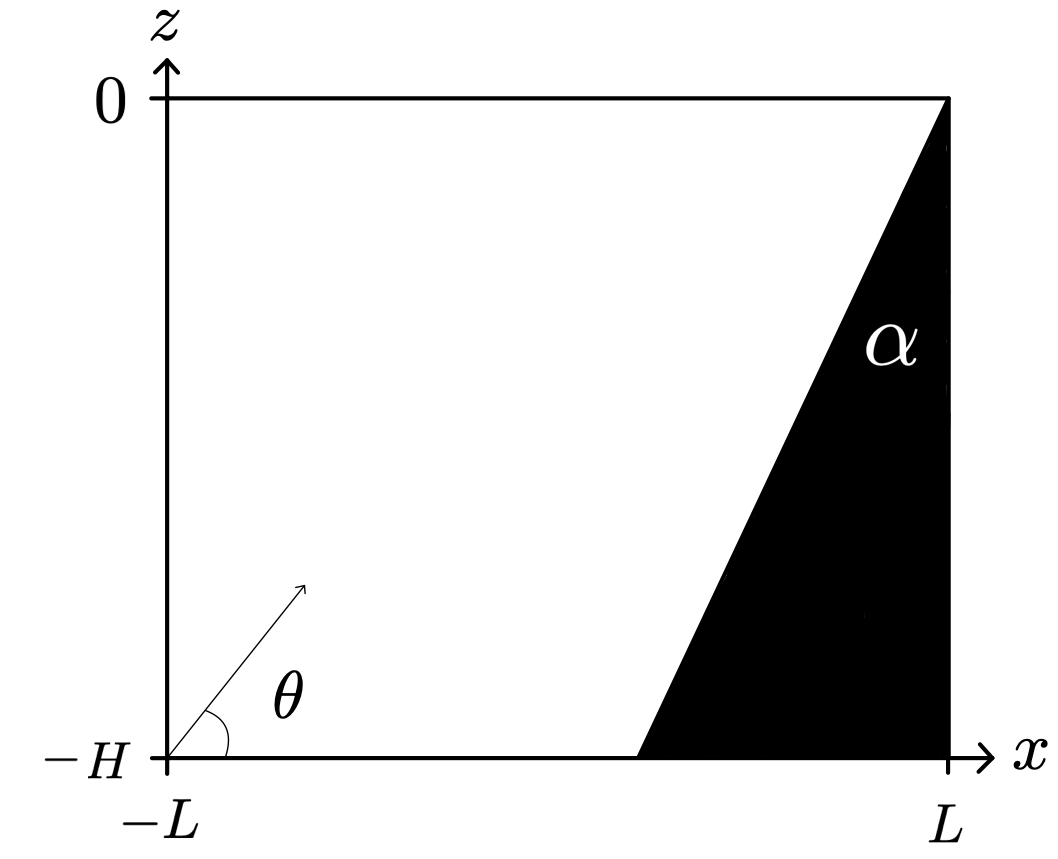
\includegraphics[width=0.7\linewidth]{Images/left2}
  \label{fig:4a}
  \caption{}
\end{subfigure}%
\begin{subfigure}[t]{.5\textwidth}
  \centering
  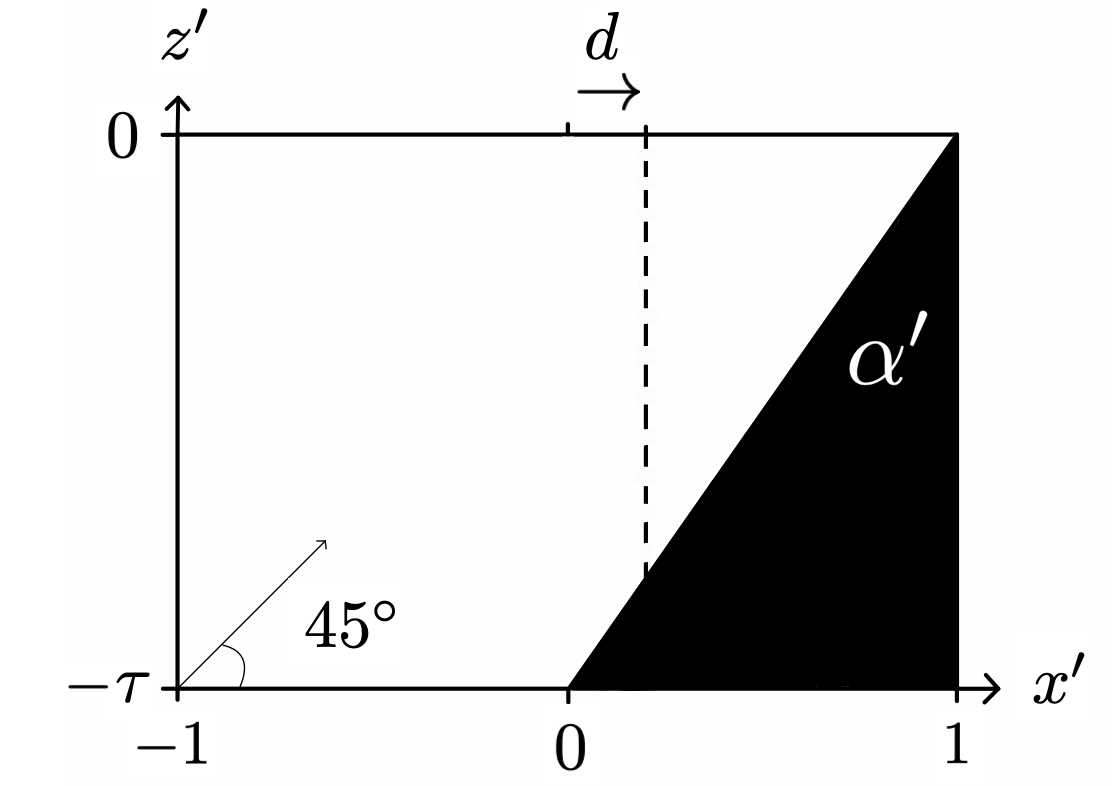
\includegraphics[width=0.7\linewidth]{Images/right2}
  \label{fig:4b}
    \caption{}
\end{subfigure}
\caption{Trapezoidal domain (a) before and (b) after a rescaled change in geometry. The arrow in the bottom left of both diagrams illustrates an internal wave ray propagating at an angle $\theta$ and $45$ degrees respectively. As consistent with literature (Maas \emph{et al.} \protect\hyperlink{ref 11}{1997}), $d=0$. Based on Brouzet (\protect\hyperlink{ref 9}{2016}).}
  \label{fig:4}
\end{figure} \\
Consider a closed container of length $2L$ and height $H$ with the right-hand side boundary tilted. To study the propagation of waves in such a basin, Maas \emph{et al.} (\protect\hyperlink{ref 11}{1997}) introduced a new spatial coordinate: $x = Lx', z = Lz'/\lambda$. Under this rescaling, the geometry of the domain changes:
\begin{align*}
\begin{split}
x \in [-L, L] \longrightarrow x' \in [-1, 1], ~~~~~~~~
z \in [-H, 0] \longrightarrow z' \in [-\tau, 0], 
\end{split}
\end{align*}
where $\tau = -\lambda H/L$. The titled boundary has parameter $s = 1 - d$ which describes the horizontal distance covered by the slope. Under this geometry, it is much easier to perform ray tracing as the rays will always propagate at an angle of $45^{\circ}$ with respect to the horizontal. Taking $N, f, H$ and $L$ as fixed parameters, the rescaled depth $\tau$ therefore changes as a result of frequency, $\omega$, only.

Under these new spatial coordinates, equation \eqref{eq:3.2} becomes, 
\begin{align}\label{eq:3.5}
\frac{\partial^2\psi}{\partial x'^2} - \frac{\partial^2\psi}{\partial z'^2} = 0,
\end{align}
with $\psi = 0$ on the boundaries. As before, this leads to the solution for $\psi$. Now, by considering the properly scaled reduced pressure (Lam \& Maas \hyperlink{ref 18}{2008}), one finds, 
\begin{align}\label{eq:3.6}
\psi(x', z') = f(x' + z') - g(x' - z'), ~~~~~~p = f(x'+z') + g(x'+z').
\end{align}
Now an appropriate domain and wave equation have been established, properties under which IWAs form can be explored. First, consider an arbitrary position $(x_0, 0)$ and follow the characteristics around the domain from characteristic (A) to (D) as seen in Figure \ref{fig:5}. Then,
\begin{equation*}
\begin{split}
A&: ~~~~ z' = -x' + c_A ~~ \text{with}  ~~~ c_A = x_0 = z_1 + x_1,\\
B&: ~~~~ z' = x' + c_B ~~~~ \text{with}  ~~~ c_B = z_1 - x_1 = -\tau - x_2,\\C&: ~~~~ z' = -x' + c_C ~~ \text{with}  ~~~ c_C = -\tau + x_2 = z_3 - 1,\\
D&: ~~~~ z' = x' + c_D ~~~~ \text{with}  ~~~ c_D = z_3 + 1 = -x_4.\\
\end{split}
\end{equation*}
Equating coefficients, $c_i$, one arrives at the relation, 
\begin{align*}
x_ 4 = x_0 - 2 - 2x_1 + 2\tau.
\end{align*}
By considering the equation for characteristic (A) and noting that the slope has equation $z' = \tau(x'-1)/s$ where $s = 1 -d$ as defined above, one finds,
\begin{align*}
x_1 = \frac{\tau + sx_0}{s + \tau}.
\end{align*}
By rearranging the above two equations and equating $x_0 = x_4 = x^*$ (a closed orbit), 
\begin{align*}
x^* = \frac{(\tau + s)(\tau -1) - \tau}{s},
\end{align*}
which can be examined for a range of $s$ values. To be consistent with Figure \ref{fig:4}(b), consider $s = 1$. Moreover, note that restrictions are imposed on the domain such that $-1 < x^* < 1$. Then,
\begin{align}\label{eq:3.7}
x^* = (\tau + 1)(\tau -1) - \tau ~~~ \implies ~~~ 1 < \tau < 2.
\end{align}
Thus, there is a continuous range of frequencies for which a closed cycle of rays, an $internal$ $wave$ $attractor$, form as depicted in Figure \ref{fig:5}. This then implies a $(1,1)$ attractor forms for forcing frequencies, $1/\sqrt{2} < \omega/N < 2/\sqrt{5}$ which is considered throughout. This cycle occurs given that the wave ray is initially launched on the wave attractor cycle. Now, consider the case where $x_0 \neq x^*$ such that $x_0 = x^* + \delta$ where $0 < \delta < 1 - x^*$. Following the characteristics from this point, $x_4$ becomes, after $n$ cycles, 
\begin{align*}
x_4 = x^* + \delta \bigg( \frac{\tau - 1}{\tau + 1}\bigg)^n.
\end{align*}
As $n \rightarrow \infty$, $x_0 \rightarrow x^*$ and so, despite starting some distance, $\delta$, away, eventually, the ray will converge onto the path of the wave attractor. This implies that the internal-wave energy that was initially distributed over the whole domain will become increasingly concentrated around this IWA. 

A range of values of $\tau$ have been established for the existence of an IWA but is this true for all reflections? Consider again, a characteristic orbit where $(x_0, 0)$ begins on the slope and after one orbit, arrives at the slope some distance away from the wave ray launching point, $(x_4, z_4)$. Recall, that $\alpha$ is the angle of the slope measured with the vertical and $\theta$ is the angle of energy propagation with respect to the horizontal. By considering the geometry of the characteristics and the domain as in Figure \ref{fig:4}(a), and taking $a = 1/\tan\alpha$ and $b = 1/\tan\theta$, the ray hits the boundaries at,
\begin{align*}
(x_0, z_0)&: ~~ x_0 = x_0, &&z_0 =ax_0\\
(x_1, z_1)&: ~~ x_1 = x_0 - \frac{z_0 - z_1}{b} = \frac{(b-a)x_0 - H}{b}, ~~~~~~~ &&z_1 = -H\\
(x_2, z_2)&: ~~x_2 = -L, &&z_2 = z_1 + b(x_1 - x_2) = (b-a)x_0 - 2H + Lb\\
(x_3, z_3)&: ~~ x_3 = x_2 - \frac{z_2}{b} = -2L + \frac{2H - (b-a)x_0 }{b}, ~~ &&z_3 = 0\\
(x_4, z_4)&: ~~ x_4 = \frac{2(H - Lb) + (a-b)x_0}{a+b}, &&z_4 = ax_4
\end{align*}
where $x_4$ has been calculated by solving $z_4 = ax_4 = b(x_3-x_4)$. For a closed orbit to exist, 
\begin{align*}
x_0 = x_4 \implies x_4 = \frac{H}{b} - L.
\end{align*}
By definition, the Iteration method (Traub \hyperlink{ref 44}{1964}) states that $x_{n+1} = g(x_n)$ will converge iff $|g'(x)| < 1$. By adopting this method and taking $x_4 = g(x)$ then an IWA will exist if and only if, 
\begin{align}\label{eq:3.8}
\abs{g'(x)} = \abs{\frac{a-b}{a+b}} = \abs{\frac{\cos(\theta + \alpha)}{\cos(\theta - \alpha)}} \equiv \frac{1}{\gamma} < 1.
\end{align}
Thus, this condition is satisfied for all focusing reflections, $\gamma > 1$. Focusing domains will therefore facilitate the existence of IWAs.
\begin{figure}[h!]
\centering
\begin{subfigure}[t]{.5\textwidth}
  \centering
  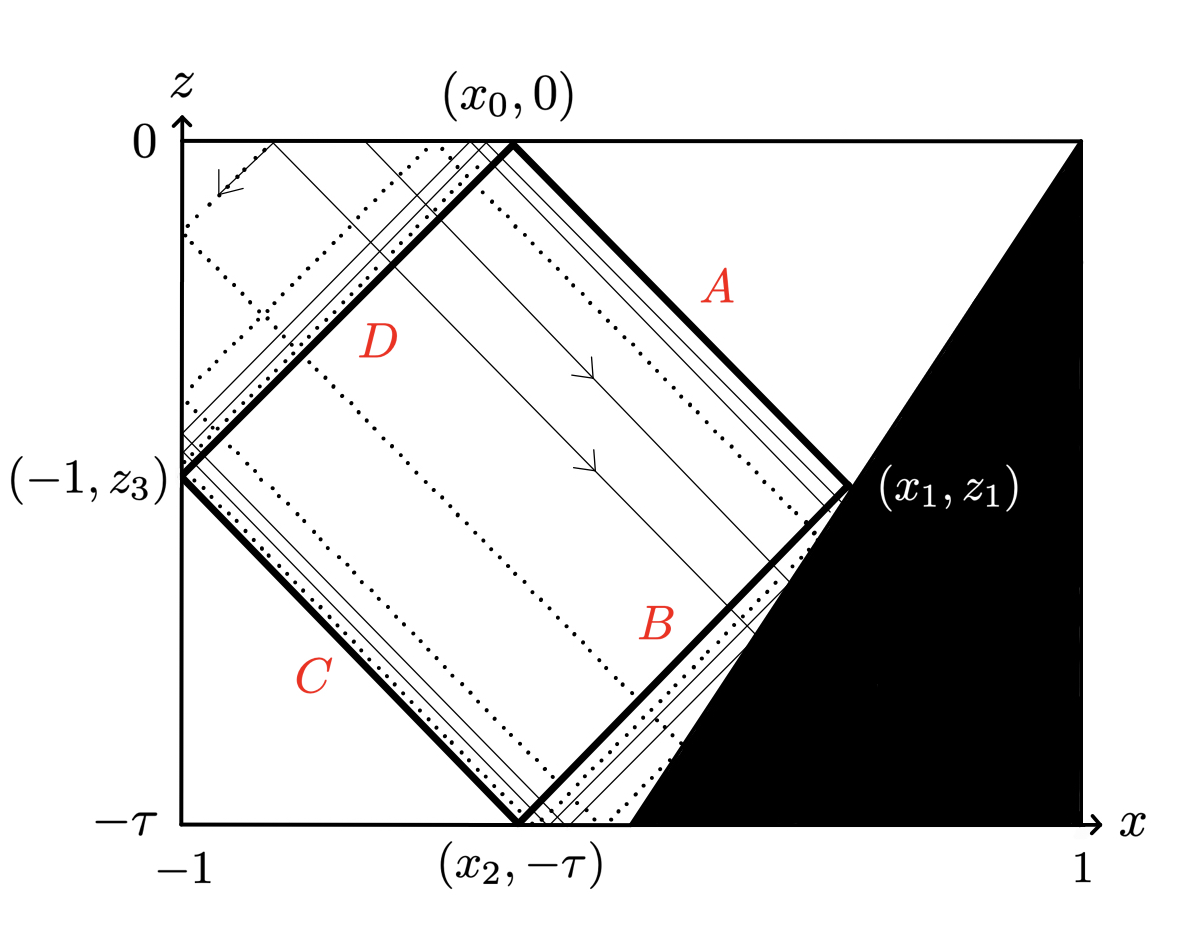
\includegraphics[width=1\linewidth]{Images/iwa diagram.jpeg}
  \caption{Ray theory prediction.}
  \label{fig:sub1}
\end{subfigure}%
\begin{subfigure}[t]{.5\textwidth}
  \centering
  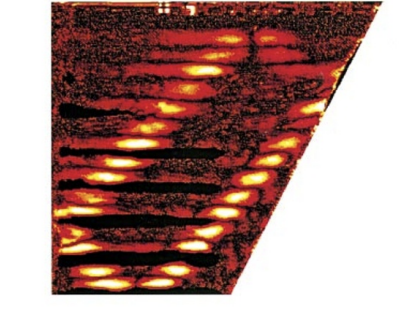
\includegraphics[width=0.875\linewidth]{Images/iwa experiment}
  \caption{Experiment.}
  \label{fig:sub2}
\end{subfigure}
\caption{Trapezoidal domain filled with stratified fluid. Dimensions as in Figure \protect\ref{fig:4}(b). Figure (a) illustrates the convergence onto a wave attractor (solid black line). Based on Maas \emph{et al.} (\protect\hyperlink{ref 11}{1997}). (b) An experiment by Maas \emph{et al.} (\protect\hyperlink{ref 11}{1997}) shows the difference between maximally displaced dye lines and their initial horizontal state in the standing phase, 9 minutes after oscillation of the tank began.}
\label{fig:5}
\end{figure}\\
Attractors studied so far reflect off both the surface and the slope once. This is known as a $(1,1)$ attractor as depicted in Figure \ref{fig:5}. Generally, attractors are denoted $(m, n)$ where $m$ is the number of reflections at the surface (top or bottom) and $n$ is the number of reflections on the sloping side wall (or vertical wall). A $(2, 1)$ attractor and a \emph{point attractor} is depicted in Figure \ref{fig:6}. A point attractor ray reflects into the corner of the basin where all of its energy is concentrated. 
\begin{figure}[h!]
\centering
\begin{subfigure}[t]{.5\textwidth}
  \centering
  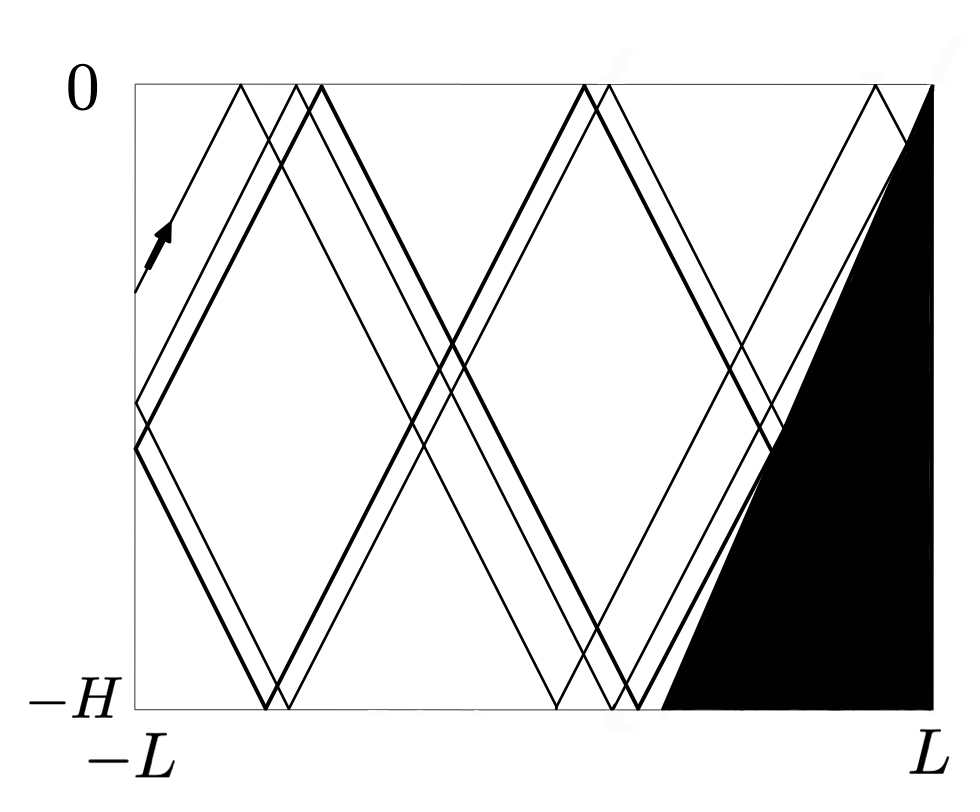
\includegraphics[width=0.78\linewidth]{Images/other attractors.jpeg}
  \caption{A (2,1) attractor.}
  \label{fig:sub1}
\end{subfigure}%
\begin{subfigure}[t]{.5\textwidth}
  \centering
  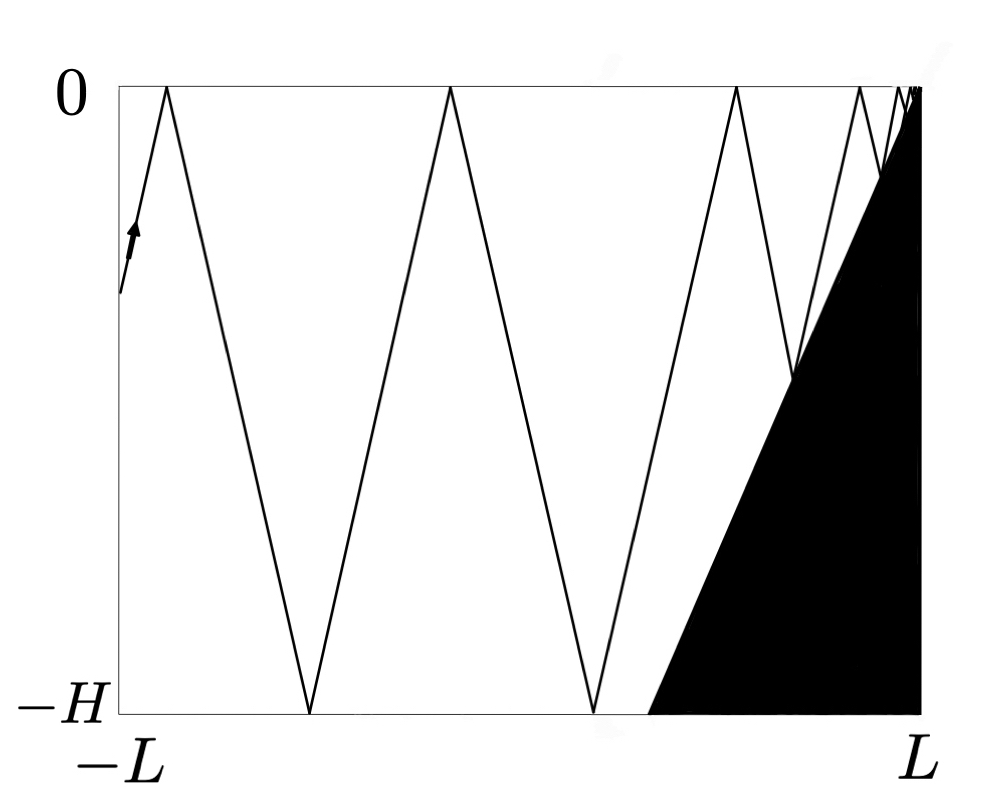
\includegraphics[width=0.8\linewidth]{Images/other attractors 2.jpeg}
  \caption{A point attractor.}
  \label{fig:sub2}
\end{subfigure}
\caption{Convergence towards different attractors. (a) A point attractor initiated at $\theta = 58^{\circ}$. (b) A (2,1) attractor initiated at $\theta = 75^{\circ}$. Dimensions, $H/2L = 2/3, d = 0.32$ and $\alpha = 26^{\circ}$. Based on Brouzet (\protect\hyperlink{ref 9}{2016}).}
\label{fig:6}
\end{figure}

By \eqref{eq:3.8}, focusing prevails over defocusing; only attractors with an odd value of $n$ will be observed. Even values of $n$ are known as \emph{global resonances} where one reflection from the sloping wall is focusing, the second is defocusing and a closed cycle forms. Physically, these are standing waves. It is important to note that the wave equation is a spatial structure only: time does not appear directly. For this reason, ray tracing should not be considered as a process that evolves in time. 

\subsection{Fundamental Intervals}
Recall from equation \eqref{eq:3.6}, 
\begin{align}
\psi = f(x'+z') - g(x'-z'), ~~~~~ p = f(x'+z') + g(x'-z'),
\end{align}
where $f$ and $g$ are the partial pressures (Sibgatullin \hyperlink{ref 19}{2019}). Applying the condition, $\psi = 0$, along the surface implies $f = g$ but for this condition to be true at different points on the boundary, it must be true that the value of $f$ is conserved between the incident characteristic and reflected characteristic. This is what sets the value at the reflected characteristic. 

Lam \& Maas (\hyperlink{ref 18}{2008}) considered a real-valued function, $f$. This then provides a standing wave solution with the surface pressure, $p_s(x') = f(x') + g(x') = f(x') + f(x') = 2f(x)$. However, the partial pressure, $f$, is preserved along characteristics. So, when following the internal wave ray, the value of $f$ passed between neighbouring surface intervals is the same. For this reason, they concluded that it is not necessary to specify the pressure on the whole boundary but only within a \emph{fundamental interval}, the interval between two successive surface intersections. By specifying the pressure within this interval, the pressure over the whole surface is also specified as illustrated in Figure \ref{fig:7}.
\begin{figure}[h!]
\centering
\begin{subfigure}[t]{.5\textwidth}
  \centering
  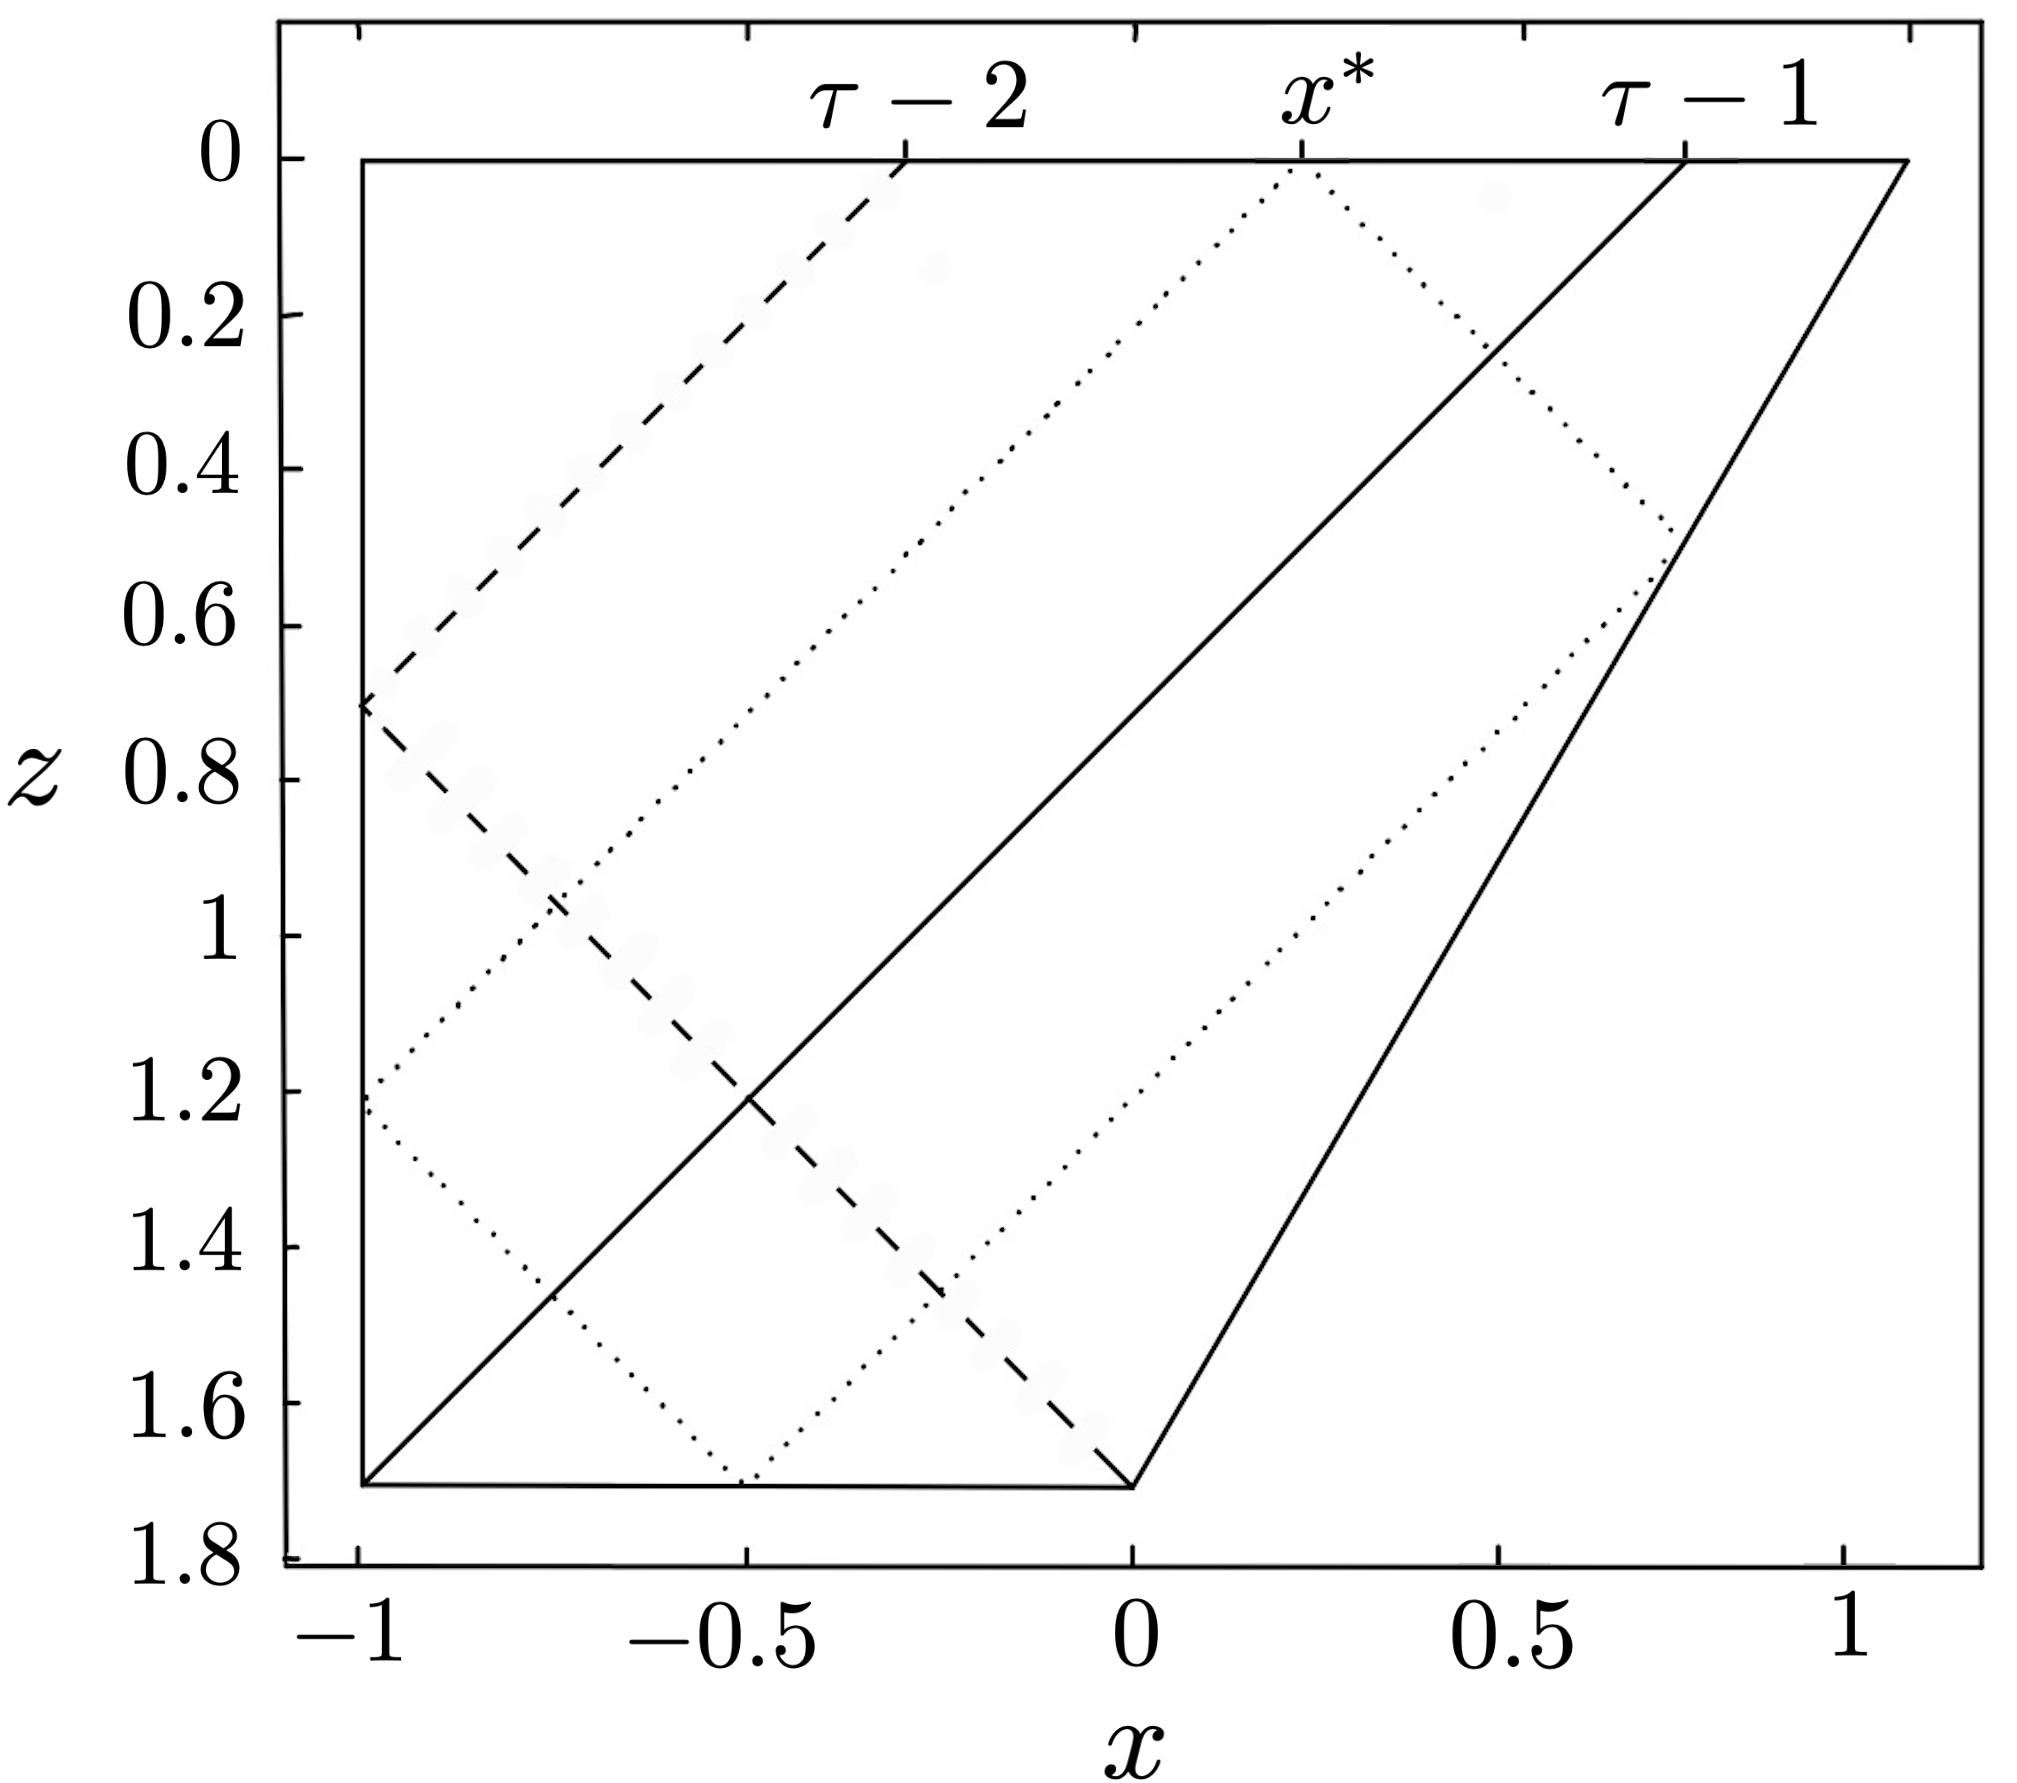
\includegraphics[width=0.78\linewidth]{Images/drawings}
  \label{fig:sub1}
  \caption{}
\end{subfigure}%
\begin{subfigure}[t]{.5\textwidth}
  \centering
  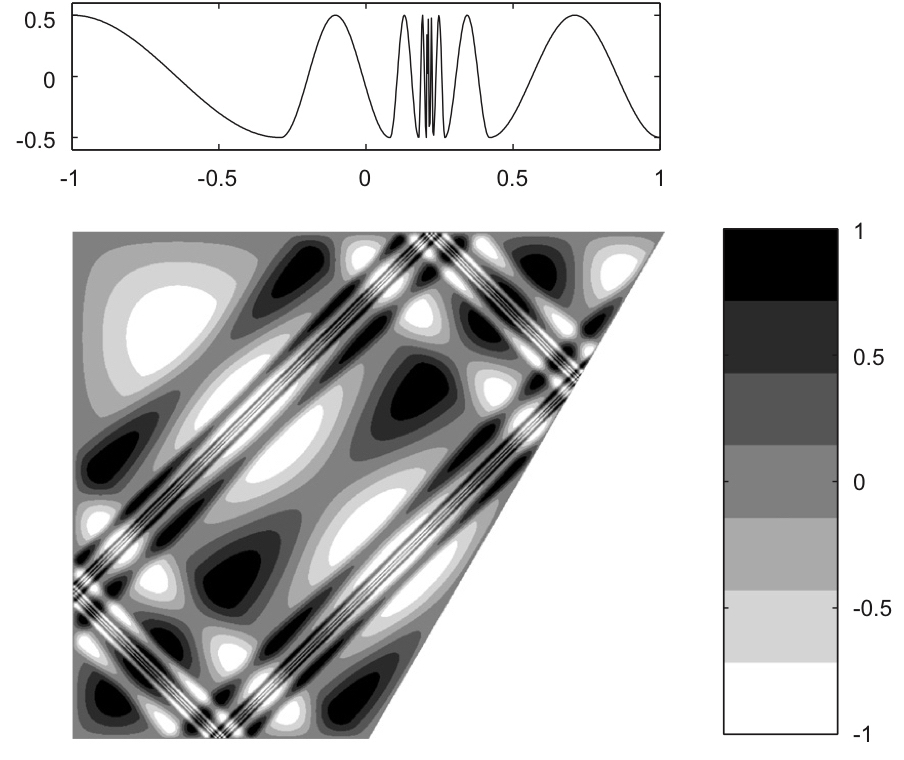
\includegraphics[width=0.82\linewidth]{Images/internal wave attractor 2.jpeg}
  \label{fig:sub2}
  \caption{}
\end{subfigure}
\caption{(a) Points on the surface of the domain where primary fundamental intervals can be specified. The attractor has surface reflection at $x^* = \tau^2 - \tau - 1$ as in \eqref{eq:3.7}. (b) Standing wave solution $\psi(x, z)$ for a surface pressure, $p_s(x') = 2f(x)$ which is specified within the two fundamental intervals in (a). Then, the whole pressure distribution along the surface (top panel) can be inferred. $\psi$ is depicted by the gray scale to the left (Lam \& Maas \protect\hyperlink{ref 18}{2008}).}
\label{fig:7}
\end{figure}\\
Figure \ref{fig:7} illustrates the largest of these intervals and is known as the \emph{primary} fundamental interval. They are obtained by taking a single wave ray from the bottom corners of the domain and following its characteristic until it reaches the upper boundary. The primary fundamental intervals for this given domain are $x \in [-1,\tau-2]$ and $x \in [\tau -1, 1]$. By specifying $f(x)$ on these intervals, the remainder of $f(x)$ can be inferred. Thus, $\psi(x,z)$ can be constructed using an iterative procedure with the function $f$ specified on these fundamental intervals at one of the boundaries of the region. 

\subsection{Travelling Wave Solution}
Recall that ray tracing does not depend on time and so the streamfunction is a standard pattern that appears to be “blinking”. This notion of “blinking” was first introduced by Maas \emph{et al} (\hyperlink{ref 17}{1995}) due to the lack of time propagation along the rays. It appears undesirable to specify the pressure merely on the two fundamental intervals with no link to actual forcing. Lam \& Maas (\hyperlink{ref 18}{2008}) revisited both these problems by considering the travelling wave solution.

\subsubsection{The “Blinking” Problem}
First, consider the “blinking" problem: is it possible to construct \emph{propagating} solution? For such solutions to exist, $f$ must be complex. The specified streamfunction on the primary fundamental intervals can be decomposed into Fourier modes such that,
\begin{align*}
\cos(ax) = \frac{1}{2}\exp(iax) + \frac{1}{2}\exp(-iax) \equiv f_R + f_L.
\end{align*}
Then, the rays can be determined by two types: those that propagate left and those that propagate right from this interval. The complex value of $f$ associated with these rays are $f_L$ and $f_R$ respectively. Thus, the infinite web of constant $f$ has been divided into two semi-infinite webs propagating with constant $f_L$ or $f_R$. These should be interpreted as the complex $f$ and $-g$ in the original derivation. Then, the complex streamfunction can be computed using equation \eqref{eq:3.6}. Finally, to obtain a time evolution of the IWA, one needs to evaluate $\Psi(x', z', t') = \psi(x',z')\exp(it')$ where $t'$ is dimensionless such that $t' = \omega t$. Doing so produces a series of images of the IWA and the propagation of waves emitted from the fundamental intervals can be clearly seen (Brouzet \protect\hyperlink{ref 9}{2016}; Lam \& Maas \hyperlink{ref 18}{2008}).

\subsubsection{The Forcing Problem}
In physical systems, forcing is not always restricted to intervals like that of the fundamental intervals. For this reason, one explores the solution when forcing is applied to the entire domain; $x' \in [-1,1]$ as consistent with experiments. In order to replicate the forcing of a wave-maker, Lam \& Maas (\hyperlink{ref 18}{2008}) suggests a superposition of partial solutions from the varying fundamental intervals. Indeed, this is possible as the streamfunctions are solutions of the linear problem. 

The first two solutions, $\psi_1$ and $\psi_{-1}$, are obtained from the two primary fundamental intervals. Then next two solutions, $\psi_2$ and $\psi_{-2}$, are obtained from the \emph{first} secondary fundamental intervals (found by following the boundaries of the primary intervals right and left). The $nth$ solution is then $\psi_{n+1}$ and $\psi_{-(n+1)}$. Altogether, the total streamfunction is given by,
\begin{equation*}
\psi = \sum_{n=1}^{N} (\psi_n + \psi_{-n}). \\
\end{equation*} 
Using this method, one obtains a series of images at different dimensionless times that clearly illustrate the propagation. 

Possibly the most interestingly aspect of internal wave rays in a closed domain is that it's an ill-posed Cauchy problem. Remarkably, Maas (\hyperlink{ref 20}{2009}) obtained an exact analytic solution of an internal wave attractor in a trapezoidal domain which exhibited a self-similar spatial structure. This self-similar solution was expressed in terms of a countable set of infinite Fourier coefficients. Of course, the above findings are for the inviscid, non-diffusive case. To understand IWAs in real world processes, one has to take into account viscosity. 
\section{The Role of Viscosity and Dissipation}
\label{sec:4}
So far, linear inviscid waves have been considered as a basis for understanding IWAs. However, much of the excitement and physicality of wave attractors arises due to viscous effects. Interestingly, the dispersion relation for internal waves does not relate $\omega$ to one wavenumber but to a spectrum of all wavenumbers. In physical processes, this is not possible and so, viscosity plays a role. 

\subsection{Viscous Decay Along an Internal Wave Beam}
\label{sec:4.1}
Consider a non-rotating, stratified, viscous fluid (Thomas \& Stevenson \hyperlink{ref 21}{1972}; Tabaei \& Akylas \hyperlink{ref 22}{2003}; Voisin \hyperlink{ref 23}{2003}). Equations \eqref{eq:2.1} - \eqref{eq:2.3} reduce to,
\begin{align*}
\frac{\partial u}{\partial t} + \frac{1}{\rho_0}\frac{\partial p}{\partial x} &= \nu \nabla^2u, \\
\frac{\partial w}{\partial t} + \frac{1}{\rho_0}\frac{\partial p}{\partial z} - b &= \nu \nabla^2w, \\
\frac{\partial b}{\partial t} + N^2w &= 0, \\
\nabla \cdot \mathbf{u} &= 0,
\end{align*}
where the tildes have been omitted and $b = -g(\rho - \rho_0)/\rho_0$ is the new buoyancy variable. Similar to the inviscid case, it is suitable to obtain a streamfunction, $\psi$, that describes the behaviour of the waves in the system. Introducing $\psi$ where $\mathbf{u} = (-\frac{\partial \psi}{\partial z},\frac{\partial \psi}{\partial x})$ and substituting gives,
\begin{align}\label{eq:4.1}
\begin{split}
\frac{\partial}{\partial t} \nabla ^2 \psi - \frac{\partial b}{\partial x} - \nu \nabla^4 \psi &= 0, \\
\frac{\partial b}{\partial t} + N^2\frac{\partial \psi}{\partial x} &= 0. \\
\end{split}
\end{align}
Recall for internal waves, the beams are inclined at $\theta$ with the horizontal and are perpendicular to the wavevector, $\mathbf{k}$. It is suitable to introduce a new coordinate system that aligns with the beam in the $(x,z)$ plane. For simplicity take $N = 1$ and introduce the coordinate $\xi$ in the direction of $\mathbf{c}_g$ and $\eta$ in the direction of $\mathbf{c}_p$ so that $\xi \perp \eta$ (Hazewinkel \hyperlink{ref 24}{2010}). Then,
\begin{align*}
\xi = x\sin\theta + z\cos\theta, ~~~~~~
\eta = x\cos\theta - z\sin\theta.
\end{align*}
Substituting into \eqref{eq:4.1} gives, 
\begin{align*}
\begin{split}
\frac{\partial}{\partial t} \nabla ^2 \psi - \frac{\partial b}{\partial \xi}\sin\theta- \frac{\partial b}{\partial \eta}\cos\theta  - \nu \nabla^4 \psi &= 0, \\
\frac{\partial b}{\partial t} + \frac{\partial \psi}{\partial \xi}\sin\theta + \frac{\partial \psi}{\partial \eta}\cos\theta &= 0. \\
\end{split}
\end{align*}
Now, assume that the viscosity, $\nu$, is small, i.e the length scale over which the viscous decay is happening is small compared with the length scale over which the sinusoidal components of the wave are occurring. Then, $\psi$ and $b$ can be expanded using a power series. Further, by seeking plane wave solutions (Hazewinkel \hyperlink{ref 24}{2010}), one can write, 
\begin{align}\label{eq:4.2}
\begin{split}
\psi = [\psi_0 + \nu\psi_1 + \nu^2\psi_2 + \ldots ] \exp(-i\omega t), ~~~~~ b = [b_0 + \nu b_1 + \nu^2
b_2 + \ldots]\exp(-i\omega t).
\end{split}
\end{align}
It can be assumed that viscosity controls the beam width so one can introduce a scaled along-beam parameter, $\chi$, such that,
\begin{align}\label{eq:4.3}
\chi = \frac{\nu \xi}{2\sin\theta},
\end{align}
where $2\sin \theta$ is for analytic convenience. By considering small viscosity there will be gradual changes in the $\xi$ direction and fast changes in the $\eta$ direction. Substituting $\psi$, $b$ and $\chi$ from \eqref{eq:4.2} and \eqref{eq:4.3} and ordering in powers of $\nu$ gives, 
\begin{align*}
&(\nu^0):&&\frac{\partial \psi_0}{\partial \eta} = ib_0,\\
&(\nu^1): &&\omega \frac{\partial \psi_1}{\partial \eta} - i\omega b_1 = -\frac{\partial \psi_0}{\partial \chi}, \\
&(\nu^1): &&i \omega \frac{\partial^2 \psi_1}{\partial \eta^2} + \omega \frac{\partial b_1}{\partial \eta} = -2 \frac{\partial^4 \psi_0}{\partial \eta^4} - \frac{\partial b_0}{\partial \chi},
\end{align*}
using the dispersion relation to simplify. By inspection, viscosity will only play a role in the $\eta$ direction, i.e. the direction of the beam width. Eliminating between variables and integrating,
\begin{align*}
\begin{split}
\frac{\partial^4 \psi_0}{\partial \eta^4} = i \frac{\partial^2 \psi_0}{\partial \chi \partial \eta}~~~ \implies ~~~\frac{\partial^3 \psi_0}{\partial \eta^3} = i \frac{\partial \psi_0}{\partial \chi} + g(\chi).
\end{split}
\end{align*}
Note that $b$ satisfies this equation when $g(\chi) = 0$ so one proceeds by setting $g(\chi) = 0$ in the above equation. By making the ansatz $\psi_0 = G(\eta)F(\chi)$, the following holds,  
\begin{align*}
\frac{G_{\eta\eta\eta}}{G} = i\frac{F_{\chi}}{F} = const. = -ik^3.
\end{align*}
As with most problems, the aim is to obtain wave-like solutions with wavenumber $k$ and so, it is suitable to set the constant to $-ik^3$ so that it is consistent with such solutions. Thus,
\begin{align*}
\psi_0 = A\exp(ik\eta -k^3\chi),
\end{align*}
where $A$ is a constant. By recalling the dependence of $\nu$ on $\chi$, the effect of viscosity on the wave amplitude can be observed; the amplitude of the wave decays exponentially in the direction of $\mathbf{c}_g$. Now, by considering a linear superposition of these solutions, the general solution can obtained, 
\begin{align}\label{eq:4.4}
\psi_0 =  \int_{-\infty}^{\infty} A(k) \exp\big( ik\eta - \frac{\nu k^3}{2\sin\theta} \xi \big) \,dk.
\end{align}
Hence, higher wavenumber components decay more rapidly. Thus, for small-amplitude internal waves, it is observed that the projection of energy onto high wave numbers as a result of geometric focusing can be balanced by viscous dissipation at high wave numbers. As seen, viscosity controls the thickness of the IWA branches but what is the equilibrium thickness of such branches?

\subsection{A Model for the Thickness of an Internal Wave Attractor}
\label{sec:4.2}
Indeed, by introducing viscosity, one can obtain a relationship between the width of the branches of the attractor and various other parameters in the problem (Grisouard \emph{et al.} \hyperlink{ref 25}{2008}). Figure \ref{fig:8}(b) schematically illustrates the propagation of a beam of internal waves as a result of a virtual point source and the thickness of the attractor is clearly seen.

The structure of the IWA is governed by the evolution of a wave packet travelling around the attractor. The wave length of this wave packet defines a scale which can be used to infer the equilibrium thickness of the IWA. As explored in Rieutord \emph{et al.} (\hyperlink{ref 12}{2001}), it can be argued that this thickness is characterised by the focusing parameter, $\gamma$, and viscous diffusion. In between focusing reflections, diffusion is the only physical process that acts on the attractor. By the diffusion scaling law, $\sigma(d\sigma/dt) = C\nu$ where $C$ is a constant and $\sigma$ is the wavelength. Then,
\begin{align*}
\sigma \frac{d\sigma}{dt} = \sigma \frac{d\sigma}{d\xi} \frac{d\xi}{dt} = \sigma \frac{d\sigma}{d\xi} \frac{\sigma N\cos\theta}{2\pi} ~~~ \implies ~~~ \sigma^2 \frac{d\sigma}{d\xi} = \frac{2\pi C\nu}{N\cos\theta},
\end{align*}
where $d\xi/dt = N\cos\theta/k = N\sigma \cos\theta/2\pi$. Now, one can integrate along the wave attractor from $\xi = 0^+$ to $\xi = L^{-}_a$, i.e. from just after the focusing point to just before it (Grisouard \emph{et al.} \hyperlink{ref 25}{2008}). Here, $L_a$ is the perimeter of the attractor in the direction of energy propagation, i.e. in the $\xi$ direction. Doing so gives, 
\begin{align}\label{eq:4.5}
\sigma^3_n(L^{-}_a) - \sigma^3_n(0^+) = 6\pi C \frac{\nu L_a}{N\cos\theta}, 
\end{align}
where $n$ denotes the $n$th orbit of the wave packet. Recalling from equation \eqref{eq:2.9},
\begin{align}\label{eq:4.6}
\gamma = \frac{\sigma_n(L^{-}_a)}{\sigma_{n+1}(0^+)}.
\end{align}
For a wave attractor at equilibrium, $\sigma_{n+1}(0^+) = \sigma_{n}(0^+)$ and so, by substituting and rearranging \eqref{eq:4.5} with \eqref{eq:4.6}, it follows, 
\begin{align*}
\sigma(0^+) = C'(\gamma^3 - 1)^{-\frac{1}{3}} \bigg(\frac{\nu L_a}{N\cos\theta} \bigg)^{\frac{1}{3}},
\end{align*}
where $C' = (6\pi C)^{1/3}$. Thus, the equilibrium thickness at any point along the attractor is,
\begin{align*}
\sigma(\xi) = C' \bigg(\frac{1}{\cos\theta}\bigg)^{\frac{1}{3}}\bigg(\frac{\nu L_a}{N} \bigg)^{\frac{1}{3}} \bigg( \frac{\xi}{L_a} + \frac{1}{\gamma^3 - 1}\bigg)^{\frac{1}{3}}.
\end{align*}
Normalising the width of the attractor by its perimeter and using the dispersion relation, 
\begin{align}\label{eq:4.7}
\begin{split}
\frac{\sigma(\xi)}{L_a} &= C'\bigg(1 - \frac{\omega^2}{N^2}\bigg)^{1/6} \bigg( \frac{\nu}{N L_a^2}\bigg)^{1/3} \bigg( \frac{\xi}{L_a} + \frac{1}{\gamma^3 -1} \bigg)^{1/3}.
\end{split}
\end{align}
Hence, the ratio of the width of the attractor to its perimeter scales as $(\nu / NL_a^2)^{1/3}$. By considering two trapezoidal domains with fixed viscosity, one can alter the size of the domain so that the perimeter of the attractor, $L_a$, is larger and thus, increases the ratio $\sigma/L_a$. Similarly, domains with different viscosities can be observed and compared (Brouzet \emph{et al.} \hyperlink{ref 26}{2016}). 
\begin{figure}[h!]
\centering
\begin{subfigure}[t]{.5\textwidth}
  \centering
  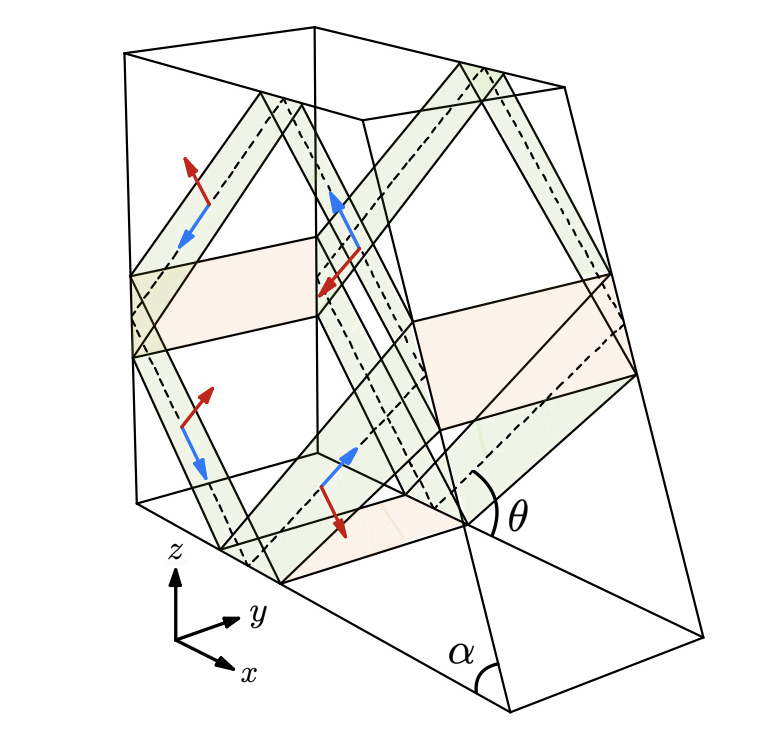
\includegraphics[width=0.72\linewidth]{Images/dissipation.jpeg}
  \label{fig:sub1}
  \caption{}
\end{subfigure}%
\begin{subfigure}[t]{.5\textwidth}
  \centering
  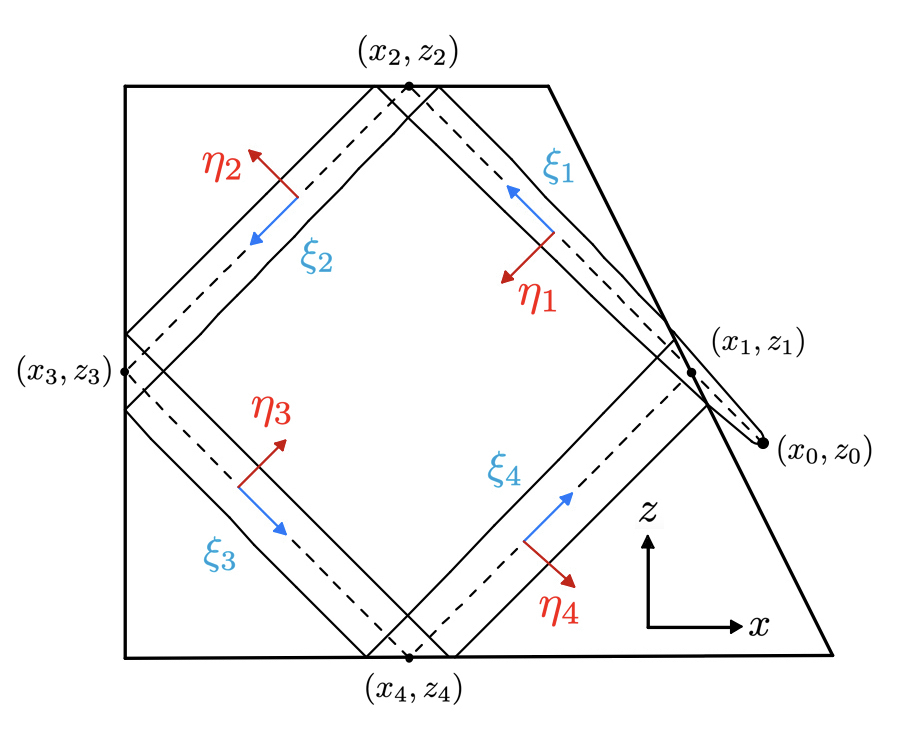
\includegraphics[width=0.84\linewidth]{Images/dissipation 2.jpeg}
  \label{fig:sub2}
  \caption{}
\end{subfigure}
\caption{Schematic drawing of a trapezoidal domain in (a) 3D and (b) its side view in 2D and 3D. Dashed lines represent the theoretic inviscid wave attractor orbit. The viscous wave attractor interacts with the solid boundaries of the domain and free surface ($z = h$). $(x_0, z_0)$ illustrates the position of the virtual source. Phase propagation occurs along $\eta_n$ (red arrows) and energy propagation occurs along $\xi_n$ (blue arrows) for $n = 1, 2, 3, 4$. The thickness of the wave attractor in the energy propagation direction is due to viscous damping. Based on Beckebanze \emph{et al.} (\protect\hyperlink{ref 8}{2017}).}
\label{fig:8}
\end{figure}

The shape of the equilibrium wave attractor in the classical trapezoidal set-up is not only dependent on the properties of the stratified fluid ($\nu$, $N$) but also on the geometry of the tank ($W$, $L_p$, $\alpha$). Relation \eqref{eq:4.7} is satisfied with sufficient accuracy for a linear regime for the range of parameters typical of laboratory experiments. However, viscous friction at the boundaries also induces additional dissipation which distorts this scaling. 

\subsection{Viscous Damping by Rigid-Wall Friction}
Hazewinkel \emph{et al.} (\hyperlink{ref 27}{2008}) constructed a model for a wave attractor spectrum at equilibrium. The model studied a propagating wave packet in a trapezoidal domain. Energy at low wave numbers were initially injected into the domain and as the energy propagated, these wave numbers transitioned into larger wave numbers due to focusing. Recall from equation \eqref{eq:4.4} that higher wave numbers are dissipated by viscosity more quickly. Thus, they justified the equilibrium state to have occurred as a result of a balance between the injected wave numbers and the viscous damping.

However, their theoretical prediction for the 2D steady state attractor did not fully describe the experimental results they found; the model only considered internal shear dissipation and neglected dissipation at the rigid boundaries. Despite their theory resembling the findings in their experiments, the lack of rigid wall dissipation introduced an inconsistency. The motivation to study dissipation in the domain came from simulations by Brouzet \emph{et al.} (\hyperlink{ref 26}{2016}) which demonstrated increased dissipation at the lateral boundaries (green in Fig \ref{fig:8}(a)). For this reason, one considers results found by Beckebanze \emph{et al.} (\hyperlink{ref 8}{2017}) and considers a situation where the IWA loses energy to the domain walls. First, consider a linearly stratified Boussinesq fluid inside a trapezoidal domain, $D$, where, 
\begin{align*}
D = \Big\{ (x,y,z) \in \mathbb{R}~ | -l_y \leq y \leq l_y, ~~-l_x \leq x \leq l_x,~~ 0 \leq z \leq \text{min} [h, (l_z-x)\tan\alpha] \Big\},
\end{align*}
as seen in Figure \ref{fig:8}(a) where $h$ denotes the height of the domain. Consider the internal wave motion to be confined to a neighbourhood around the theoretical inviscid wave attractor denoted by the dashed line in Figure \ref{fig:8}. 

In such a domain, there is a free-slip boundary condition at $z = h$ and no-slip condition, $\mathbf{u} = \mathbf{0}$, at the remaining side walls. Now, introduce a scaling such that $(x,y,z)$ have characteristic length scale $L_0$ which is also assumed to be the length scale of the viscous wave attractor in the cross-beam direction. For realistic results, the dimensional width of the container, $W = 2l_yL_0$, must be of the same order of magnitude as the cross-beam length scale of the wave attractor, $L_0$. 

Now, by considering monochromatic forcing with small-amplitude motions, the full system of linear, dimensionless equations becomes (Beckebanze \emph{et al.} \hyperlink{ref 8}{2018}), 
\begin{align*}
\frac{\partial\mathbf{u}}{\partial t} = - \nabla p + b \mathbf{\hat{z}} + \delta^2\nabla^2\mathbf{u} + \mathbf{f}e^{-it},
~~~~~~ \frac{\partial b}{\partial t} = -N^2w, ~~~~~~ \nabla \cdot \mathbf{u} = 0.
\end{align*}
where $N$ has been rescaled such that $N = \pm 1/\sin\theta$. The forcing $\mathbf{f} = \mathbf{f}(x,z)$ is a localised source along the y-axis, outside the domain as illustrated in Figure \ref{fig:8}(b). Recall that dissipation takes place in two types of viscous layers: shear layers as discussed above and boundary layers at the rigid boundaries. Here, $\delta = \frac{d_0}{L_0} \ll 1$, is the non-dimensional Stokes boundary layer width, with $d_0 = \sqrt{\nu/\omega_0}$. The thickness of a boundary layer in stratified fluid is given by (Schlichting \& Gersten \hyperlink{ref 28}{2000}),
\begin{align*}
d_0 = \frac{1}{\mu} \sqrt{\frac{\nu}{\omega}}, ~~~~ \text{with} ~~ \mu = \sqrt{ \bigg| \frac{\sin^2\phi}{\sin^2\theta} - 1 \bigg|}.
\end{align*}
where $\phi$ is the angle of the boundary with respect to the horizontal and $\theta$ the internal wave inclination. Noting that $\delta$ is a small quantity, one can expand variables in this quantity such that, 
\begin{align*}
\mathbf{u} = \mathbf{u}_0 + \delta\mathbf{u}_1 + \mathcal{O}(\delta^2),
\end{align*}
and similarly for the pressure $p$ and buoyancy $b$. By adopting this approach, Beckebanze \emph{et al.} (\hyperlink{ref 8}{2018}) considered wave attractor branches in the domain.

\subsubsection{Wave Attractor Branches in Interior}
\label{sec:4.3.1}
By considering $(\xi, \eta)$ coordinates, it's convenient to describe the four wave attractor branches in the same rotated coordinates, $(\xi_n, \eta_n)$ where $n$ denotes the branch for $n = 1,2,3,4$. By relating to the reflection points on the attractor (Beckebanze \emph{et al.} \hyperlink{ref 8}{2017}), it follows that, 
\begin{align*}
\begin{pmatrix}
\xi_{1,3}\\
\eta_{1,3}
\end{pmatrix} = \mp
\begin{pmatrix}
\cos\theta & -\sin\theta\\
\sin\theta & \cos\theta
\end{pmatrix}
\begin{pmatrix}
x - x_{1,3}\\
z - z_{1,3}
\end{pmatrix}, ~~~
\begin{pmatrix}
\xi_{2,4}\\
\eta_{2,4}
\end{pmatrix} = \mp
\begin{pmatrix}
\cos\theta & \sin\theta\\
\sin\theta & -\cos\theta
\end{pmatrix}
\begin{pmatrix}
x - x_{2,4}\\
z - z_{2,4}
\end{pmatrix}
\end{align*}
as seen in Figure \ref{fig:8}; the dashed lines illustrate the theoretical inviscid attractor as explored in Section (\hyperref[sec:3]{3}). This corresponds to $\eta = 0$ for all wave beams. By considering the velocity component along the wave beam, $U$, and $\mathcal{O}(\delta^0)$ terms for the velocity, one can write the first IWA branch as,
\begin{align}\label{eq:4.8}
\mathbf{u}_0^{[1]} = \hat{\xi_1}U(\eta_1) = (-\cos\theta, 0, \sin\theta)~U(\eta_1), ~~~
U(\eta) = \int_{0}^{\infty} \hat{U}(k) \exp (i(k\eta - t)) \,dk.
\end{align}
Here, $k$ is the non-dimensional wave number (scaled by $1/L_0$). Moreover, $\hat{\xi}_1$ denotes the unit vector pointing along the first branch. Now, $U(\eta)$ can be rewritten in terms of the Fourier spectrum,
\begin{align*}
\hat{U}(k) = \frac{1}{2\pi}\int_{-\infty}^{\infty} U(\eta) \exp (-i(k\eta) )\,d\eta,
\end{align*}
which depends on the localised source at $(x_0, y_0)$. This quantity equals 0 for $k \leq 0$ as it is assumed that no energy propagates towards the forcing source. The main intention is to find constraints for $\hat{U}(k)$ under both geometric focusing and viscous dissipation. These can then be compared against the theory and experiments in Hazewinkel \emph{et al.} (\hyperlink{ref 26}{2016}).

This velocity will remain the same for the free-slip reflections of the attractor branches on the non-sloped boundary walls; $z=h$, $x=-l_x$, and $z=0$,
\begin{align}\label{eq:4.9}
\mathbf{u}_0^{[n]} = \hat{\xi_n}U(\eta_n) ~~~ \text{for} ~~n = 2, 3, 4.
\end{align}
The fourth wave attractor branch returns to the sloped wall where,
\begin{align}\label{eq:4.10}
\text{Re} \bigg[\bigg( \mathbf{u}_0^{[1]} + \mathbf{u}_0^{[4]}\bigg) \cdot \mathbf{\hat{n}}_\alpha \bigg] = 0,
\end{align}
is the free-slip boundary condition with $\mathbf{\hat{n}}_\alpha = (\sin\alpha, 0, \cos\alpha)$, the normal vector of the sloping wall. By calculating and recalling, $z = (l_x - x)\tan\alpha$, it follows,
\begin{equation*}
\begin{split}
\mathbf{u}_0^{[1]} \cdot \mathbf{\hat{n}}_\alpha =& - \sin(\alpha - \theta) \int_{0}^{\infty} \hat{U}(k) \exp \bigg[ ik\frac{\sin(\alpha - \theta)}{\cos\alpha}(x-x_1) - it\bigg] 
\,dk.\\
\mathbf{u}_0^{[4]} \cdot \mathbf{\hat{n}}_\alpha =& \sin(\alpha + \theta) \int_{0}^{\infty} \hat{U}(k) \exp \bigg[ ik\frac{\sin(\alpha + \theta)}{\cos\alpha}(x-x_1) - it\bigg] 
\,dk.
\end{split}
\end{equation*}
For $\theta$ defined as the angle of the wave beam propagation with the vertical, the focusing parameter changes such that $\gamma = \frac{\sin(\alpha + \theta)}{\sin(\alpha - \theta)}$. Now, by making the 
substitution $k \rightarrow \gamma k$ into $\mathbf{u}_0^{[1]} \cdot \mathbf{\hat{n}}_\alpha$, the exponential equals that of $\mathbf{u}_0^{[4]} \cdot \mathbf{\hat{n}}_\alpha$. Now, evaluating the boundary condition gives, 
\begin{align}\label{eq:4.11}
\text{Re} \bigg[\int_{0}^{\infty} \bigg( \hat{U}(\gamma k) - \hat{U}(k)\bigg) \exp \bigg[ ik\frac{\sin(\alpha + \theta)}{\cos\alpha}(x-x_1) - it\bigg]\,dk \bigg] = 0.
\end{align}
Thus, for the free-slip boundary condition to be satisfied for all time $t$, at all reflecting walls, the spectral constraint must be satisfied, 
\begin{align*}
\hat{U}(\gamma k) = \hat{U}(k).
\end{align*}
The solutions to this equation are given by $\hat{U}(k) = P(\log_\gamma(k))$ for any arbitrary period-1 function $P$ (Beckebanze \& Keady \hyperlink{ref 29}{2016}). Interestingly, for points on the inviscid internal wave attractor, all of these spectra (except $P=0$) actually produce non-integrable velocity expressions. This is consistent with Rieutord \emph{et al.} (\hyperlink{ref 12}{2001}) in their study of inertial waves in a rotating spherical shell; they illustrated that in a 2D inviscid problem, the convergence towards an attractor resulted in a non-integrable velocity field. 

Recall the exact self-similar wave attractor solution by Maas (\hyperlink{ref 20}{2009}) was expressed in terms of a countable set of infinite Fourier coefficients. A discrete spectra of $\hat{U}(k)$ is also what is obtained when considering the values for which \eqref{eq:4.8} and \eqref{eq:4.9} $are$ integrable. As already seen, this solution can be regularised by adding viscous attenuation. 

\subsubsection{Internal Shear Layer Dissipation}
The method of adding weak viscous attenuation was first studied by Thomas \& Stevenson (\hyperlink{ref 21}{1972}) and was explored for a single wave beam in Section (\hyperref[sec:4.1]{4.1}). As above, consider one wave attractor branch with velocity $U$ in the direction of energy propagation, $\xi$, and phase propagation in the $\eta$ direction. Under this coordinate system, the continuity and buoyancy equations can be combined to reveal the governing equation for $U$,
\begin{align*}
-\nabla^2U + N^2(\sin^2\theta U_{\eta\eta} + 2\cos\theta\sin\theta U_{\eta\xi} + \cos^2\theta U_{\xi\xi}) = - i\delta^2 \nabla^4U.
\end{align*}
Recall from Section (\hyperref[sec:4.3.1]{4.3.1}), $\mathcal{O}(\delta^0)$ terms were considered when calculating the velocity expression. Providing the dispersion relation, $1 = N^2\sin\theta$, holds, the equation is solved at the same order by $U(\eta)$. Beckebanze \emph{et al.} (\hyperlink{ref 8}{2017}) followed by assuming $\hat{U}_\xi \in \mathcal{O}(\delta^2) \subset \mathcal{O}(\delta)$ in order for $U$ to be a solution of $\mathcal{O}(\delta^0)$. Then, at $\mathcal{O}(\delta^2)$, the equation reduces to, 
\begin{align*}
2N^2\cos\theta\sin\theta U_{\eta\xi} = - i\delta^2 U_{\eta\eta\eta\eta}.
\end{align*}
The solution to this equation can be expressed in a similar form to \eqref{eq:4.8} such that, 
\begin{align}\label{eq:4.12}
U = \int_{0}^{\infty} \hat{U}(k, \xi) \exp (i(k\eta - t)) \,dk,~~~~ \hat{U}(k,\xi) = \hat{U}(k)\exp\bigg[-\delta^2 \frac{\tan\theta}{2}k^3(\xi - c)\bigg],
\end{align}
where $c$ is the distance to the virtual source along the $\xi$ direction. Thus, the 2D wave attractor velocity field under viscous attenuation can be derived by making the transformation, $\hat{U}(k) \rightarrow \hat{U}(k)\exp[-\delta^2 \frac{\tan\theta}{2}k^3(\xi - c)]$ in equations \eqref{eq:4.8} and \eqref{eq:4.9}. By incorporating this transformation again into equation \eqref{eq:4.11} at $(x_1,z_1)$ results in the spectral constraint, 
\begin{align}\label{eq:4.13}
\hat{U}(\gamma k) = \hat{U}(k)\exp\bigg[-\delta^2 \frac{\tan\theta}{2}k^3\lambda \bigg],
\end{align}
where the non-dimensional length of the wave attractor is denoted $\lambda = L_a/L_0$. Hence, the effect of viscosity on the spectrum $\hat{U}(k)$ results in the addition of an exponential attenuation factor that scales as $k^3$ as already established in Section (\hyperref[sec:4.1]{4.1}). It's worth commenting on the symmetry of equation \eqref{eq:4.12}; the real part of $U(\eta, \xi)$ is even around $\eta = 0$ and in contrast, the imaginary part is odd. The symmetry is broken at the sloped boundary but maintained at the remaining boundaries. All wave attractors include some form of symmetry-breaking reflections and so for the analysis, it is suitable to consider $L_a \gg L_0$ so that the asymmetry of the attractor is negligible. 

The spectral constraint for the velocity field now becomes, 
\begin{align}\label{eq:4.14}
\hat{U}(k) = P(\log_\gamma(k))\exp[-\beta_1 k^3], ~~~~~ \text{with}~~~\beta_1 = \frac{\delta^2\lambda\tan\theta}{2(\gamma^3 - 1)},
\end{align}
where, this time, the functions $P$ are continuous period-1 functions and the spectral constraint admits integrable finite-energy spectra (Beckebanze \emph{et al.} \hyperlink{ref 8}{2018}). The addition of the exponential term represents the energy dissipation from moving around the wave attractor once. This constraint is the same as the buoyancy gradient spectrum, $A(k)$, that Hazewinkel \emph{et al.}  (\hyperlink{ref 27}{2008}) obtained (upon correction of some mathematical mistakes). Although in their analysis, they achieved a good fit, their application was not correct. Upon correct application, their theory predicted the wave attractor length to be a factor 2 smaller than observed. This contrast between theory and observation illustrates the remarkable conclusion that dissipation at the rigid walls must contribute substantially.

\subsubsection{Dissipation at Lateral and Reflecting Walls}
Upon a similar analysis, Beckebanze \emph{et al.} (\hyperlink{ref 8}{2018}) obtained spectral constraints for dissipation at the lateral walls and reflecting walls of the domain. The full 3D equilibrium wave attractor spectrum that takes into account viscosity in the shear layers and at the lateral and reflecting walls is, 
\begin{align*}
\hat{U}(\gamma k) = \hat{U}(k)\exp\bigg[-\delta^2 \frac{\tan\theta}{2}k^3\lambda - \delta \big(\frac{i\sigma \lambda}{l_y}\big) + \delta\big(R_\alpha + R_0 + R_{\pi/2}\big)k \bigg],
\end{align*}
where $\sigma, R_\alpha, R_0, R_{\pi/2}$ can be found in Beckebanze \emph{et al.} (\hyperlink{ref 8}{2018}). Here, the first, second and third term are contributions of dissipation at the internal shear layer, lateral walls and reflecting walls respectively. It is therefore clear to see that the walls produce an additional exponential attenuation factor to the initially derived inviscid spectral constraint.
Solutions to the above are given by, 
\begin{align}\label{eq:4.15}
\hat{U}(k) = P(\log_\gamma(k))\exp[-\beta_1k^3 - \beta_2k -\beta_3k] ~~~~ \text{with}~~ \beta_2 = \frac{i\delta\lambda\sigma}{l_y(\gamma - 1)},
\end{align} 
and $\beta_3$ stated in Beckebanze \emph{et al.} (\hyperlink{ref 8}{2018}). Here, $\beta_1, \beta_2, \beta_3$ the additional attenuation factors.

\subsubsection{Scaling}
The scaling of wave attractors has been established in this essay (Hazewinkel \emph{et al.} \hyperlink{ref 27}{2008}) but has been a topic of much debate throughout the last two decades (Rieutord \emph{et al.} \hyperlink{ref 12}{2001}; Ogilvie \emph{et al.} \hyperlink{ref 13}{2005}; Grisouard \emph{et al.} \hyperlink{ref 25}{2008}; Brouzet \emph{et al.} \hyperlink{ref 26}{2016}). By considering a scaling argument, one can establish the dominant forms of dissipation in the wave attractor. First, consider equation \eqref{eq:4.14} for internal shear dissipation with $P = const.$. The characteristic wave length is, 
\begin{align*}
L_{0, I} = \frac{2\pi}{k_{max}} = 2\pi (3\beta_1)^{1/3} \propto \bigg( \delta^2 \frac{\tan\theta}{2}k^3\lambda \bigg)^{1/3} \propto \bigg(\frac{L_a \nu}{N_0}\bigg)^{1/3},
\end{align*}
where $\delta^2 = d^2_0/L^2_0 = \nu/(\omega_0 L^2_0)$ and $\lambda = L_a/L_0$. This result is consistent with the wave length originally found by Rieutord \emph{et al.} (\hyperlink{ref 12}{2001}) and further verified numerically by Grisouard \emph{et al.} (\hyperlink{ref 25}{2008}) which is explored in Section (\hyperref[sec:4.2]{4.2}). Now, consider equation \eqref{eq:4.15} with $\beta_1, \beta_3 = 0$, i.e. damping only by the lateral walls. The characteristic wave length is, 
\begin{align*}
L_{0, W} = \frac{2\pi}{k_{max}} = 2\pi \text{Re}(\beta_2) \propto \text{Re}\bigg( \frac{i\delta\lambda\sigma}{l_y(\gamma - 1)} \bigg) \propto \bigg(\frac{L_a}{W}\bigg)\bigg(\frac{\nu}{N_0}\bigg)^{1/2},
\end{align*}
where $W = 2l_y L_0$ has further been used. Now, the dissipation at the lateral walls becomes negligible when $L_{0,I} \gg L_{0,W}$. This is true when (Beckebanze \emph{et al.} \hyperlink{ref 8}{2018}), 
\begin{align*}
W \gg \frac{(L_a)^{\frac{2}{3}} (d_0)^{\frac{1}{3}} \sigma_0 [2 \cot \theta (\gamma^3 - 1)/3]^{\frac{1}{3}}}{2(\gamma -1)}.
\end{align*}
Then, by considering set-ups by Brouzet \emph{et al.} (\hyperlink{ref 26}{2016}) and exploring three different regimes, it follows,
\begin{enumerate}
\item For $L_a \gg W$, dissipation is dominated at the lateral walls $\implies L_{0,W} \propto L_a$.
\item For $L_a \sim W$, internal shear dissipation contributes significantly $\implies L_{0,I} \propto L_a^{\frac{1}{3}}$.
\item For $L_a \ll W$, dissipation is dominated at the reflecting walls $\implies L_{0} = const.$
\end{enumerate}

The structure of an internal wave attractor in equilibrium is therefore not only dependent on the internal shear dissipation and wave focusing but also on viscous dissipation at the rigid boundaries. In Section (\hyperref[sec:4.2]{4.2}) a relation was obtained that linked the shape of the attractor in the internal shear layers to parameters of the problem. Now, the structure also depends on the properties of the fluid ($\nu$, $\omega$ and $N$), the geometry of the domain ($W$, $L_a$ and $\alpha$) and finally, the energy input which obtains the period-1 function $P$.

\section{Non-Linear Stratification}
\label{sec:5}
Thus far, only a constant buoyancy frequency $N$ has been discussed. In order to relate to geophysical and astrophysical systems, one extends to an $N \neq const.$ case. Note that for the ray-tracing method to be used, the stratification must change over length scales that are much greater than the wavelength. This is also known as the WKB approximation (Lighthill \hyperlink{ref 31}{1978}). By adopting this approximation, one can obtain analytic solutions for the characteristics of stratification profiles. 

\subsection{Exponential Stratification}
First consider an exponential stratification such that, 
\begin{align*}
N(z) = N_0 e^{-z/h},
\end{align*}
with $kh \gg 1$ where $h$ the characteristic perturbation height (depth of the stratification). Recall that characteristics are defined by,
\begin{align}\label{eq:5.1}
\frac{dz}{dx} = \pm \sqrt{\frac{\omega^2}{N^2 - \omega^2}}, ~~~~~~~ \text{with} ~~~ \omega = \pm N\cos\theta,
\end{align}
where the angle, $\theta$, of beam energy propagation is now with respect to the vertical to keep consistent with experimental findings. To explore the behaviour of such characteristics, one can substitute $N(z)$ into \eqref{eq:5.1} and obtain the position of the wave beam, $x$, for specified forcing frequency, $\omega$. Instead, one can eliminate the frequency dependence and obtain an expression for $x$ purely in terms of the initial angle of the beam and perturbation height. By substituting for $\omega$ into equation \eqref{eq:5.1} it follows, $dx/dz = \pm \tan\theta$. Thus, the position of the wave beam can be described by,
\begin{align*}
x =  \int_{0}^{z} \frac{dx}{dz} \,dz = \int_{0}^{z}\pm \tan\theta \,dz.
\end{align*}
Using the dispersion relation, 
\begin{align*}
\begin{split}
\frac{\omega}{N} = \frac{\omega}{N_0}e^{z/h} = \pm \cos\theta &\implies \frac{1}{h}\frac{\omega}{N_0}e^{z/h} dz = \mp\sin\theta d\theta,\\
& \implies \pm \frac{1}{h}\cos\theta dz = \mp\sin\theta d\theta.
\end{split}
\end{align*}
Thus, $dz = -h \tan\theta d\theta$. Then, introducing $\theta_0$ as the angle of the beam at $z = 0$, 
\begin{align*}
x = \int_{\theta_0}^{\theta} -h \tan^2\theta \,d\theta = \int_{\theta_0}^{\theta} h(1 - \sec^2\theta) \,d\theta.
\end{align*}
Evaluating the integral and substituting for $\theta$,
\begin{align*}
x = h\bigg[ \cos^{-1}\big(e^{z/h}\cos\theta_0\big) - \frac{\sqrt{1 - e^{2z/h}\cos^2\theta_0}}{e^{z/h}\cos{\theta_0}} \bigg] + \underbrace{h(\tan\theta_0 - \theta_0)}_\text{const}.
\end{align*}
It's worth noting that $1 - e^{2z/h}\cos^2\theta_0 \geq 0$ must hold for $x$ to exist. This is equivalent to saying $\omega \leq N(z)$, i.e. the forcing frequency must be less than the buoyancy frequency which is consistent with the dispersion relation. One can plot this function (Figure \ref{fig: 9}) and observe the behaviour of two rays that are launched at the same $\theta_0$ and $h$ but are a distance $d$ apart. 
\begin{figure}[h!]
\centering
\begin{subfigure}[t]{.5\textwidth}
  \centering
  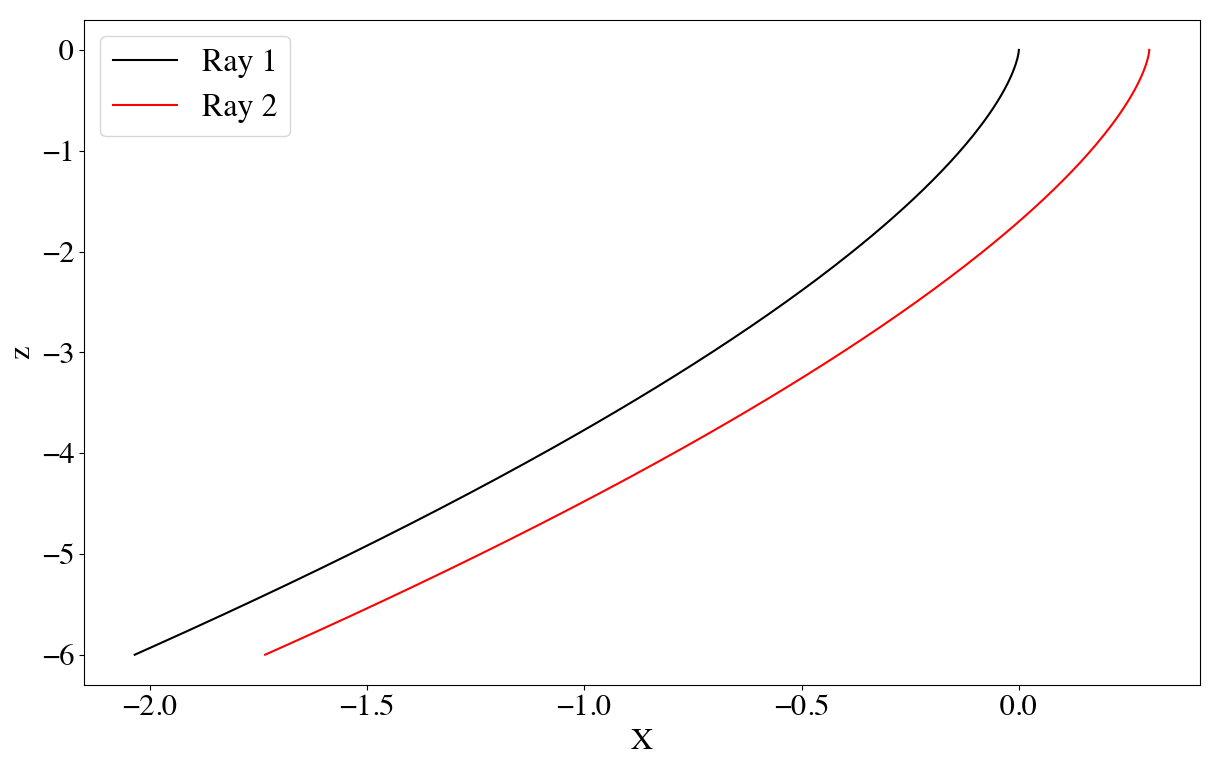
\includegraphics[width=1.055\linewidth]{Images/exponential}
  \caption{Ray theory prediction.}
  \label{fig:sub1}
\end{subfigure}%
\begin{subfigure}[t]{.5\textwidth}
  \centering
  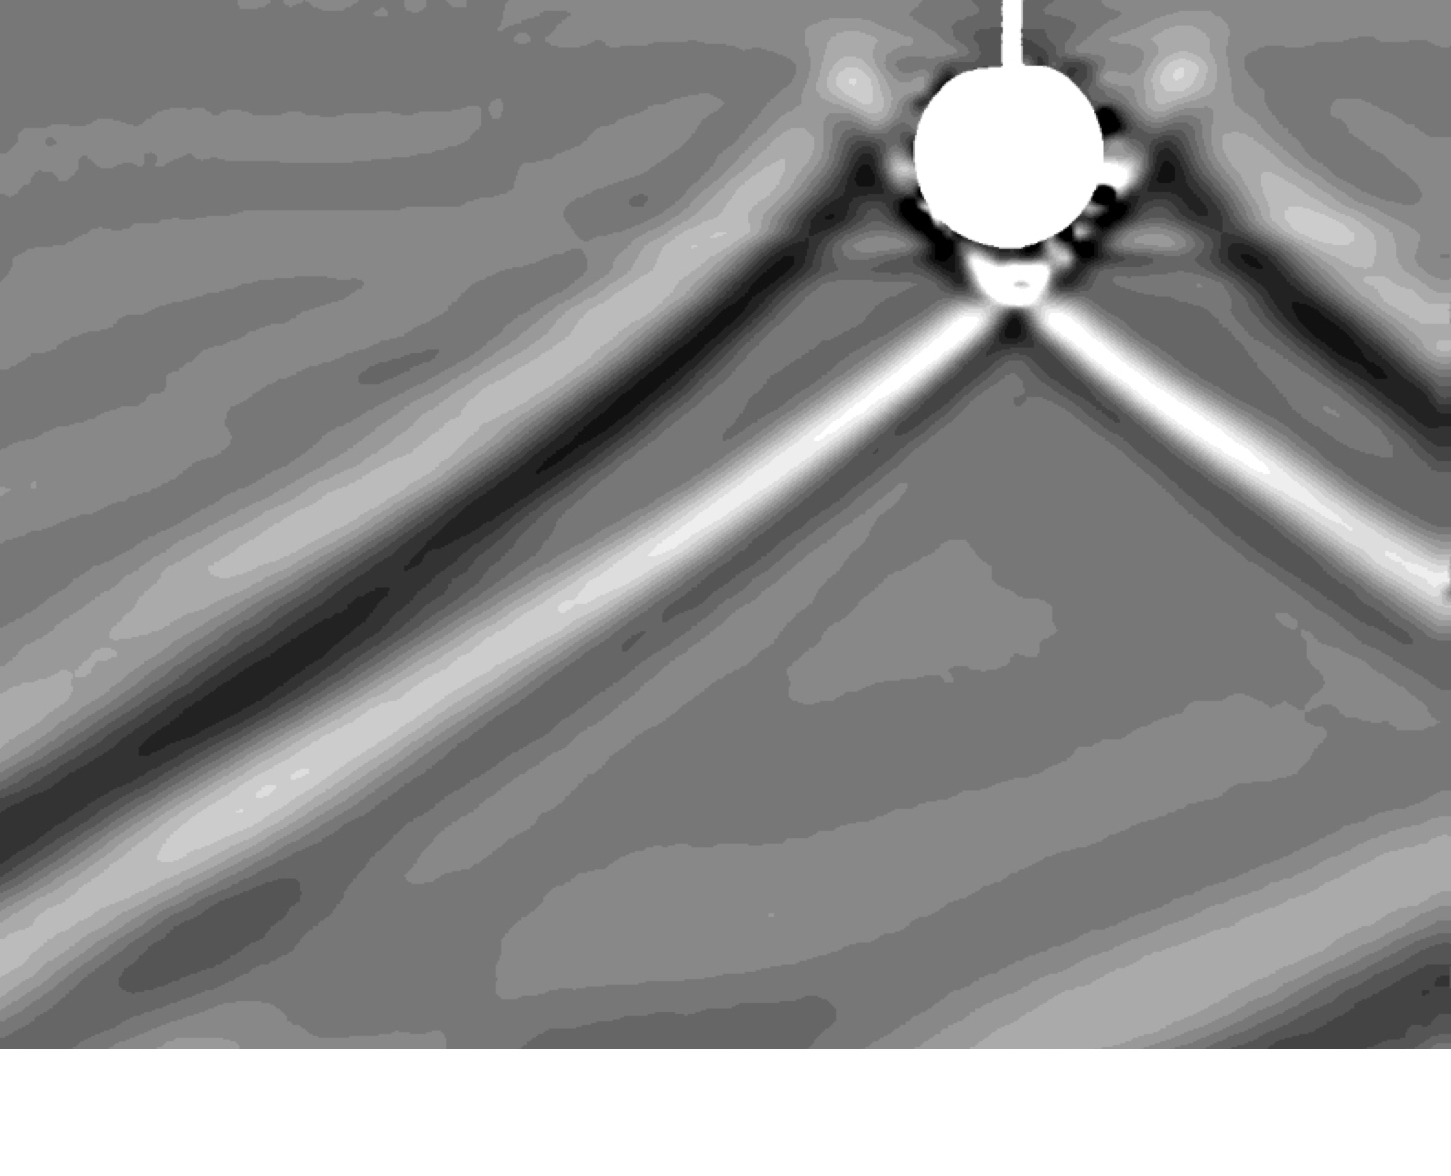
\includegraphics[width=0.8\linewidth]{Images/experiment}
  \caption{Oscillating cylinder experiment.}
  \label{fig:sub2}
\end{subfigure}
\caption{Wave beam in exponential stratification. (b) Roger (\protect\hyperlink{ref 50}{2002}).}
\label{fig: 9}
\end{figure}

As illustrated by Figure \ref{fig: 9}, the distance between two wave rays remains the same throughout but, interestingly, the wavelength decreases as the rays tend towards the horizontal. The magnitude of the group velocity, $|\mathbf{c}_g|$, can be written in terms of $\sin\theta$ for this dispersion relation and so, as the wave beam tends towards the horizontal, the group velocity will increase.

Along with an increase in the group velocity, the wavelength, $\sigma$, decreases. Eventually, both rays will become horizontal at the same height. Thus as the wavelength tends towards zero, the wavenumber will diverge. Indeed, the energy flux will be the same throughout and so this energy will be concentrated through a progressively smaller wavelength. Despite the group velocity increasing, the decreasing wavelength wins out. Hence, the energy becomes focused and as a result, non-linearities and wave breaking can form. 

Of course, in experiments, viscosity will play a role. As already established, dissipation scales with the wavenumber cubed. In physical processes, the waves will become stronger as they tend towards the horizontal when compared with the uniform stratification. However, dissipation will eventually play a role to break this high concentrated region of energy.

\subsection{Hyperbolic Stratification}
To illustrate the existence of IWAs in non-linear stratification, one considers the proposed stratification profile by Hazewinkel (\hyperlink{ref 24}{2010}),
\begin{align}\label{eq:5.2}
N^2(z) = N^2_0 + N^2_1 \text{sech}^2[(z-H/2)/h].
\end{align}
Instead of eliminating the forcing frequency, $\omega$, as done previously, consider a case of a fixed $\omega$. Substituting \eqref{eq:5.2} using equation \eqref{eq:5.1} gives, 
\begin{align*}
\pm \frac{dx}{dz} = \sqrt{\frac{1}{\omega^2}\bigg(N^2_0 + N^2_1 \text{sech}^2[(z-H/2)/h]\bigg) - 1}.
\end{align*}
By making a change of variables such that $x = \sqrt{N^2_0/\omega^2 - 1}~h x'$ and $z = H/2 + h z'$ then, 
\begin{align*}
\pm x' = \int_{}^{} \sqrt{1 + n^2\text{sech}^2(z')} \,dz',
\end{align*}
where $n^2 = N^2_1/(N^2_0 - \omega^2)$. Integrating gives, 
\begin{align}\label{eq:5.3}
\pm x' = n~ \text{arctan}\bigg(\frac{n~ \text{sinh}(z')}{\sqrt{n^2 + \text{cosh}^2(z')}}\bigg) + \text{arcsinh}\bigg(\frac{\text{sinh}(z')}{\sqrt{n^2 + 1}}\bigg) + c,
\end{align}
where $c$ is the constant of integration. As with the $N = const.$ case, the characteristics can venture in two different directions as noted by the $+$ and $-$. As before, subsequent surface positions can be calculated and constructed exactly. Figure \ref{fig:10} illustrates \eqref{eq:5.3} and \eqref{eq:5.2}. Clearly the non-linear stratification results in curved wave beams which contrasts to the $N = const.$ case. Interestingly, the wave beams deviate from their straight path when $N(z)$ changes most drastically.
\begin{figure}[h!]
\centering
\begin{subfigure}[t]{.5\textwidth}
  \centering
  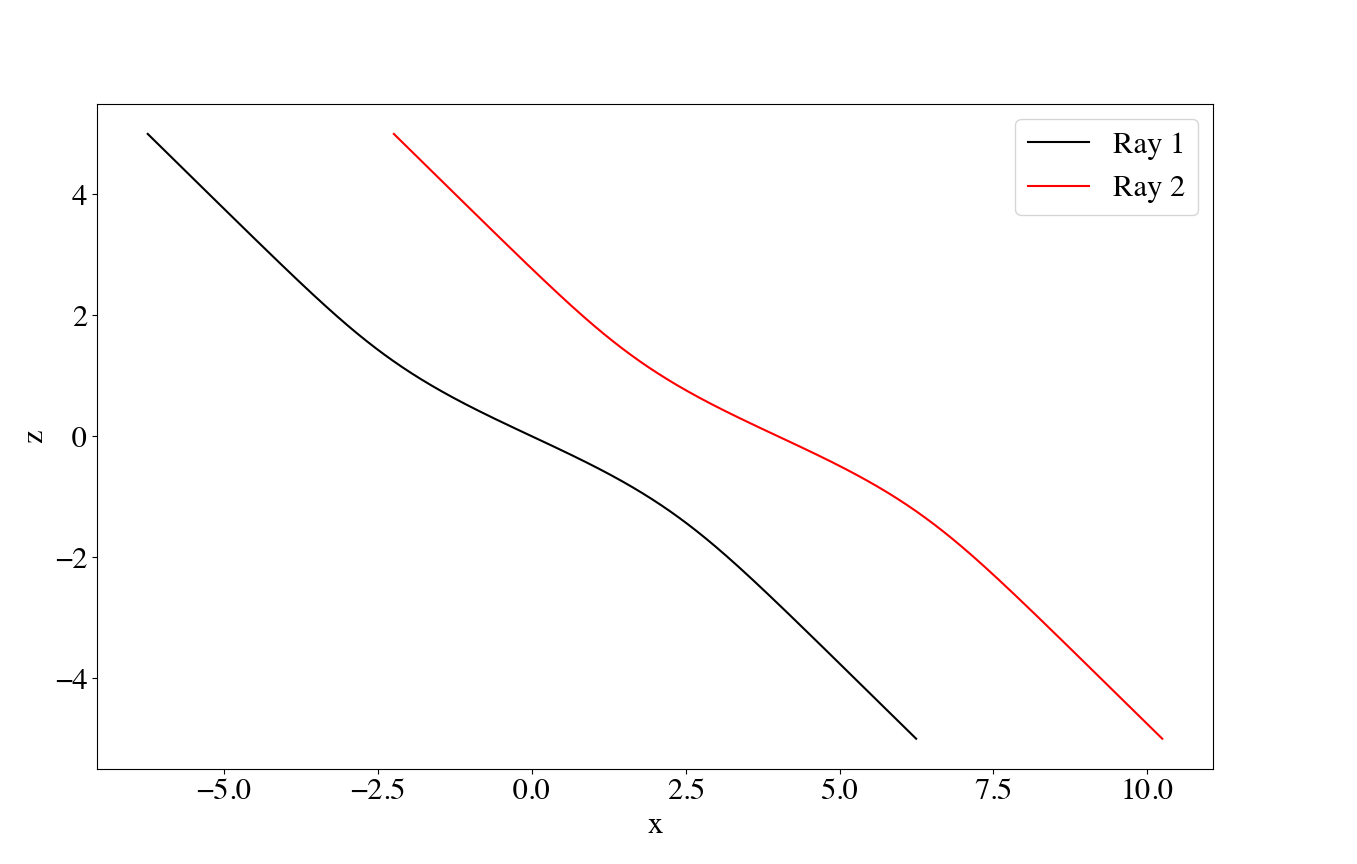
\includegraphics[width=1.1\linewidth]{Images/curve}
  \caption{Ray theory prediction}
  \label{fig:sub1}
\end{subfigure}%
\begin{subfigure}[t]{.5\textwidth}
  \centering
  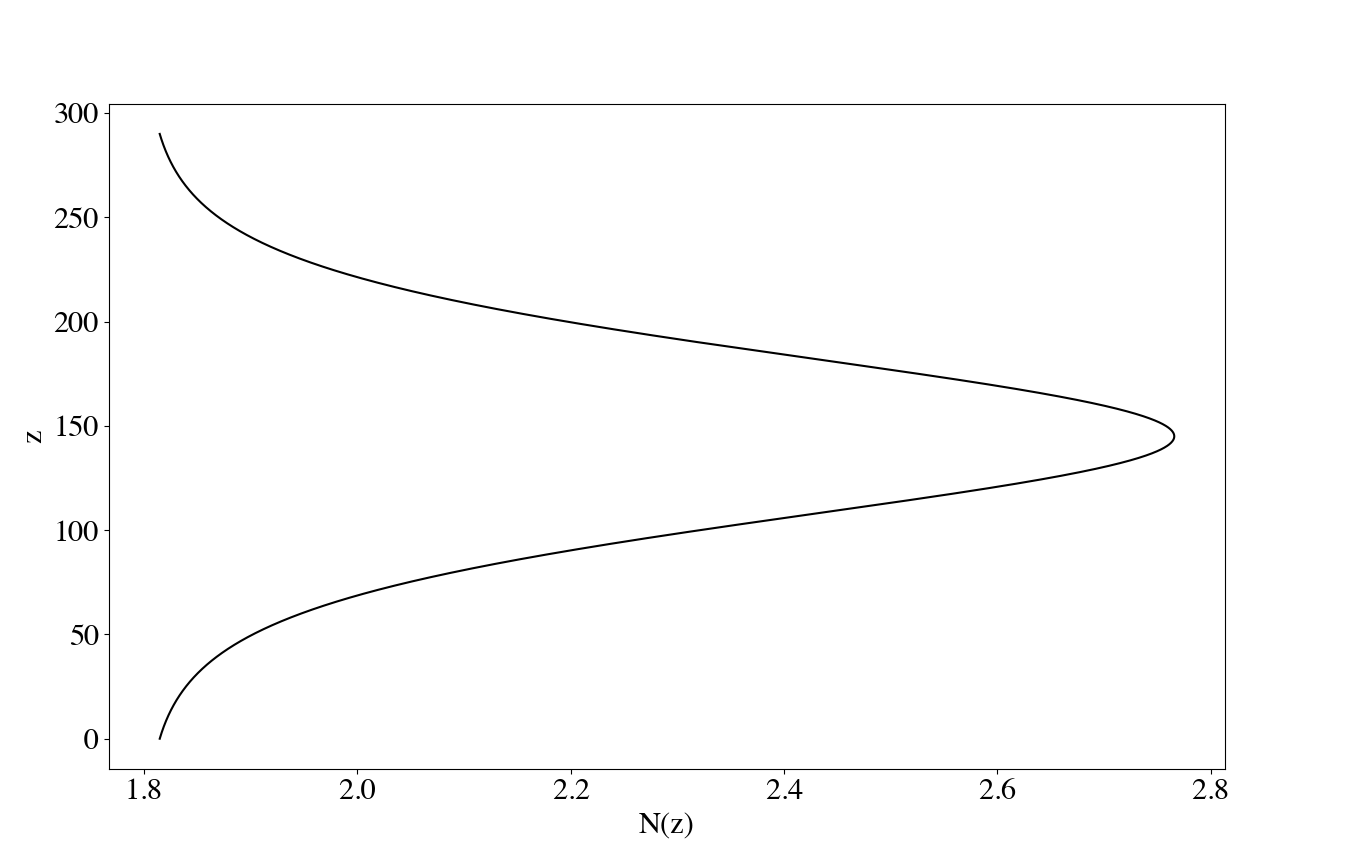
\includegraphics[width=1.1\linewidth]{Images/stratification}
  \caption{Profile of $N(z)$}
  \label{fig:sub2}
\end{subfigure}
\caption{Predictions for a wave beam with stratification, $N^2(z) = N^2_0 + N^2_1 \text{sech}^2[(z-H/2)/h]$. Parameters are fixed such that, $N_0 = 1.8$rad$s^{-1}$, $N_1 = 2.1$rad$s^{-1}$, $\omega = (2\pi/4.9)$rad$s^{-1}$, $h = 50$mm, $H=290$mm as consistent with experiments performed in Hazewinkel (\protect\hyperlink{ref 24}{2010}).}
\label{fig:10}
\end{figure}

This stratification does indeed lead to IWAs unlike the exponential case. Hazewinkel (\hyperlink{ref 24}{2010}) explored three different forcing frequencies to vary the shape of the $(1,1)$ attractor but for convenience, Figure \ref{fig:10} and \ref{fig:11} illustrate only one of these frequencies. As predicted by the ray theory, the steady state pattern observed in experiments does indeed embody the predicted curvature of the beams. Interestingly, one observes the robustness of such internal wave attractors; despite an alteration to the stratification, an IWA still exists.
\begin{figure}[h!]
  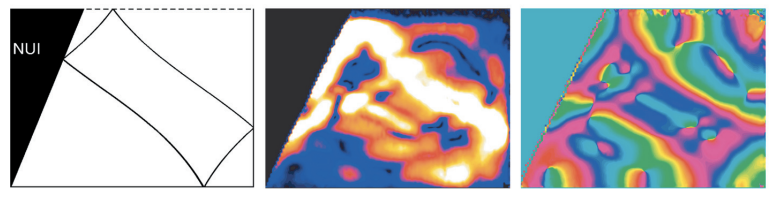
\includegraphics[scale=0.9, center]{Images/one forcing}
  \caption{An experiment for a wave beam with stratification, $N^2(z) = N^2_0 + N^2_1 \text{sech}^2[(z-H/2)/h]$. Parameters fixed such that $N_0 = 1.8$rad$s^{-1}$, $N_1 = 2.1$rad$s^{-1}$, $\omega = (2\pi/4.9)$rad$s^{-1}$, $h = 50$mm, $H=290$mm. From left to right: (i) ray tracing prediction of IWA, (ii) observations of the steady state patterns in terms of harmonic amplitude, (iii) observations of the steady state patterns in terms of phase. The internal waves are forced by horizontally oscillating a platform supporting the tank with an amplitude of $0.03$m at an adjustable frequency. Obtained by Hazewinkel (\protect\hyperlink{ref 24}{2010}).}
  \label{fig:estimated_mean}
  \label{fig:11}
\end{figure}
\section{Triadic Resonant Instability (TRI)}
\label{sec:6}
The internal waves discussed thus far have been considered under a small amplitude regime where the governing equations have been linearised. However, as the amplitude of the wave increases, various wave modes may begin interacting through the non-linear terms. Interestingly, plane waves are also solutions of the non-linear governing equations \eqref{eq:2.1} - \eqref{eq:2.3}. However, for a superposition of modes the same is not true. 

\emph{Triadic resonance} describes a phenomenon by which a triad of waves can spontaneously transfer energy to each other under certain conditions (Craik \hyperlink{ref 32}{1988}). This transfer of energy can occur at arbitrarily small but non-zero amplitudes. Consider the weakly non-linear perturbations by three periodic waves with their own wavenumber, frequency and constant amplitude:
\begin{align}
\mathbf{u} &= \mathbf{u}_0 + \mathbf{u}_1 + \mathbf{u}_2 
= \mathbf{\hat{u}}_0 e^{i(\mathbf{k}_0 \cdot \boldsymbol{x} - \omega_0 t)} + \mathbf{\hat{u}}_1 e^{i(\mathbf{k}_1 \cdot \boldsymbol{x} - \omega_1 t)} + \mathbf{\hat{u}}_2 e^{i(\mathbf{k}_2 \cdot \boldsymbol{x} - \omega_2 t)}.
\end{align}
Now, the non-linear advection term, $\mathbf{u} \cdot \nabla \mathbf{u}$, in the momentum equation \eqref{eq:2.1} gives rise to terms of the form $\exp[i((\mathbf{k}_a \pm \mathbf{k}_b) \cdot \boldsymbol{x} - (\omega_a \pm \omega_b)t)]$ where $(a, b) \in \{0, 1, 2\}$ (Bourget \emph{et al.} \hyperlink{ref 33}{2013}). For $a = b$, the disturbances do not satisfy the dispersion relation and so the net effect of these terms are less interesting. For $a \neq b$, the other terms act as forcing terms in the governing equations at second order in the linear wave amplitudes. Thus, it is expected that the non-linear interactions will lead to a gradual change in the waves when terms $\partial \mathbf{u}/\partial t$ and $\mathbf{u} \cdot \nabla \mathbf{u}$ match.

In general, three plane waves will form a resonant triad if, 
\begin{align}
s_0\omega_0 + s_1 \omega_1 = \omega_2,\\
s_0 \mathbf{k}_0 + s_1 \mathbf{k}_1 = \mathbf{k}_2,
\end{align}
where $s_0, s_1 = \pm1$. These are the temporal and spatial resonance conditions respectively. When the above holds, the interaction is known as a \emph{resonant triad}. Here, weakly non-linear interactions between any two of the waves resonantly forces the third. However, such an interaction will only excite the wave if it satisfies the dispersion relation. It is possible for the temporal resonance to hold but not all combinations of the wavenumbers will interact. Likewise, both conditions can occur even if the resulting disturbance doesn't satisfy the linear dispersion relation. Of course, the difference being whether the resulting disturbance is localised or can propagate. 

More generally, the resonance conditions and dispersion relation can be written in terms of the wavenumber components (Bourget \emph{et al.} \hyperlink{ref 33}{2013}). One can consider a primary wave, $\mathbf{u}_0$, with $(s_0, \omega_0)$ and, without loss of generality, take $s_0 = + 1$. The two secondary waves, $\mathbf{u}_1$ and $\mathbf{u}_2$, could form a resonant triad with the primary wave. Considering the dispersion relation, the resonance condition leads to, 
\begin{align}\label{eq:6.4}
s_0 \frac{\abs{k_0}}{\sqrt{k^2_0 + m^2_0}} = s_1 \frac{\abs{k_1}}{\sqrt{k^2_1 + m^2_1}} + s_2 \frac{\abs{k_0 + k_1}}{\sqrt{(k_0 + k_1)^2 + (m_0 \pm m_1)^2}}.
\end{align}
For any given primary wave, $(s_0, \omega_0)$, the solution to this equation is presented in Figure  \ref{fig:11} for every sign combination $(s_0, s_1, s_2)$. 
\begin{figure}[h!]
\centering
\begin{subfigure}[t]{.5\textwidth}
  \centering
  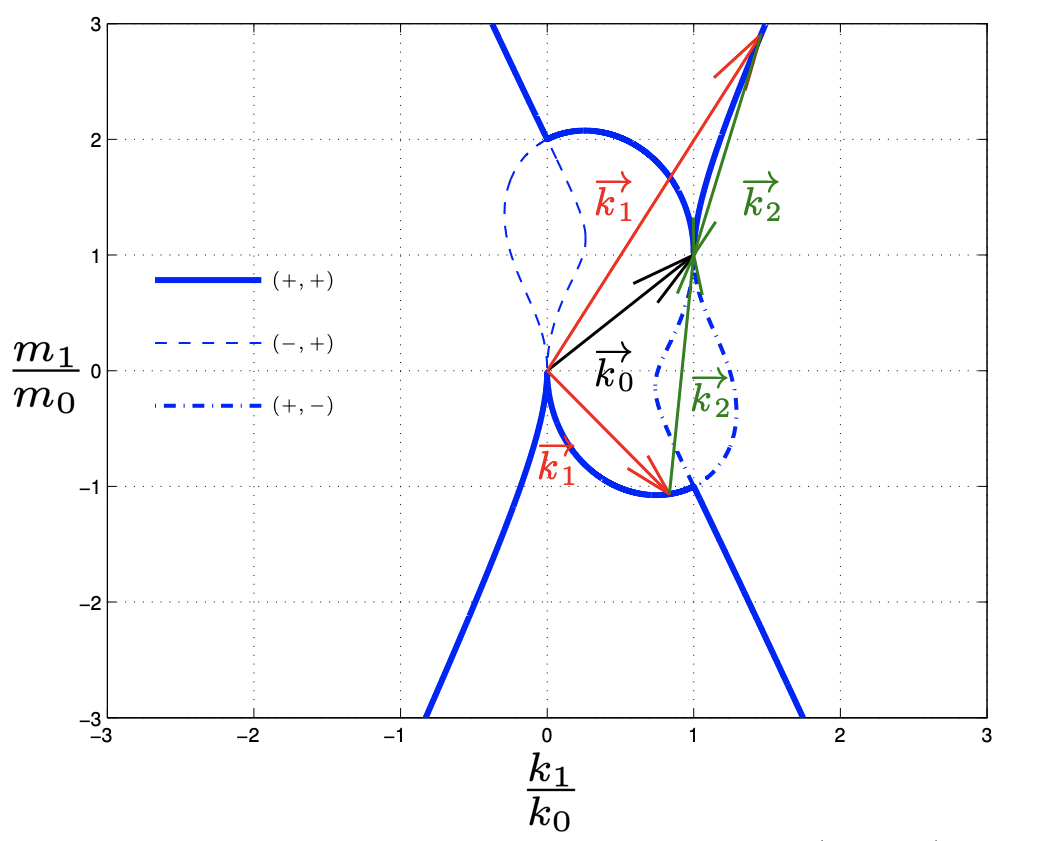
\includegraphics[width=0.9\linewidth]{Images/spatial}
  \caption{}
  \label{fig:sub1}
\end{subfigure}%
\begin{subfigure}[t]{.5\textwidth}
  \centering
  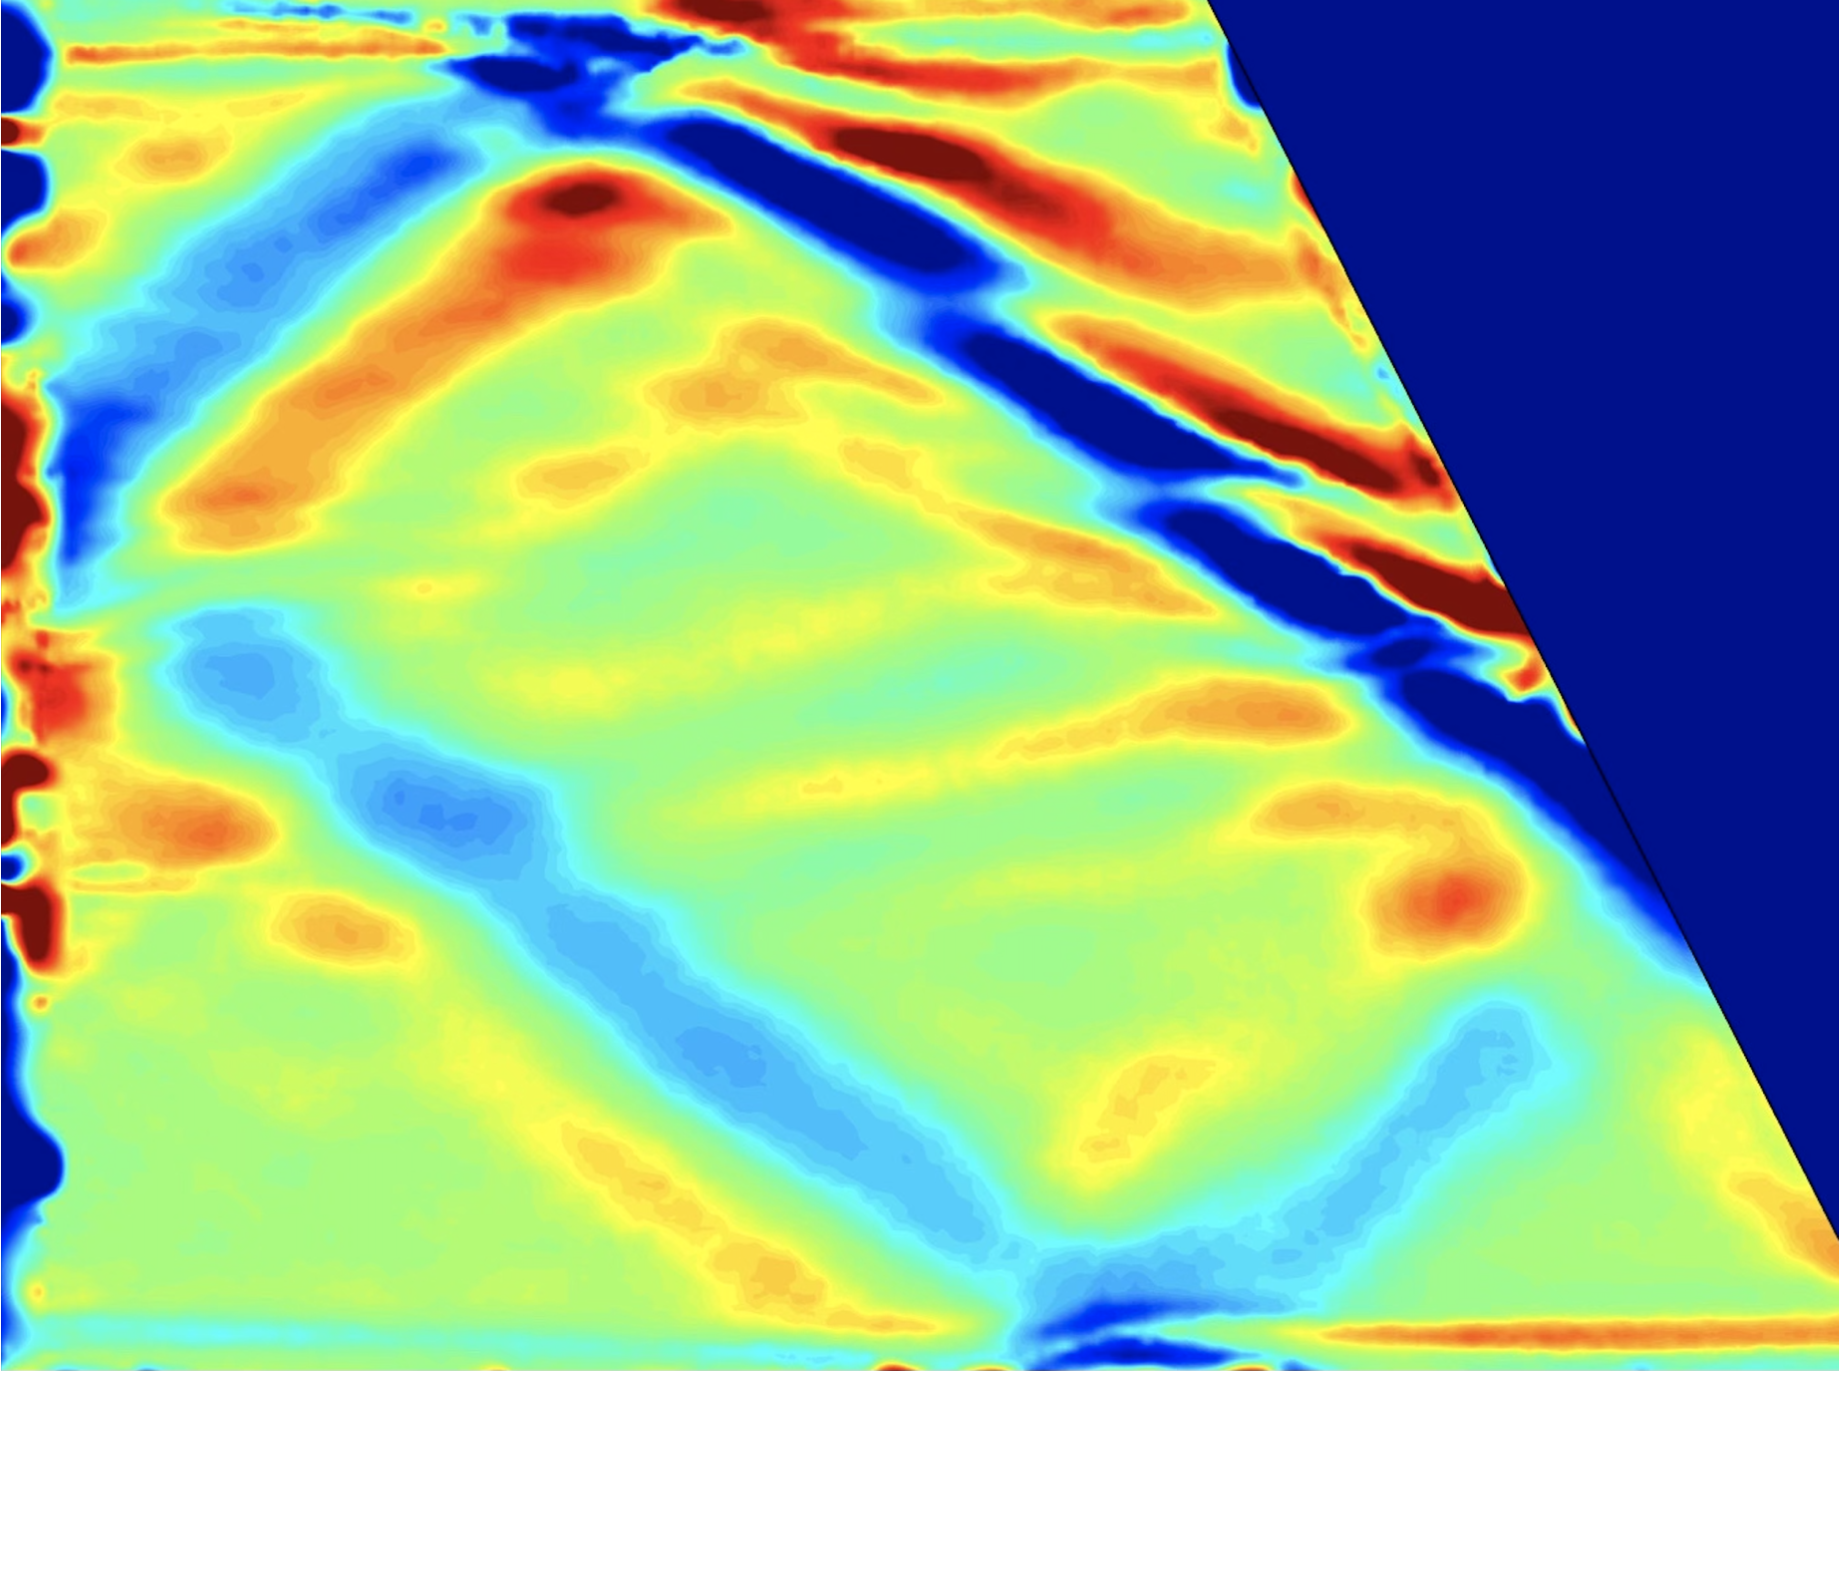
\includegraphics[width=0.81\linewidth]{Images/iwa instability 2}
  \caption{}
  \label{fig:sub2}
\end{subfigure}
\label{fig:9}
\caption{(a) Curves representing the location of $(k_1, m_1)$ that satisfy equation \eqref{eq:6.4} with three different combinations of signs. Here, the wavevector $\mathbf{k}_0 = (k_0, m_0)$ for the primary wave is given. Solid curves show where exponential growth or decay is possible and dashed curves illustrate oscillatory resonant solutions. (Bourget \emph{et al.} \protect\hyperlink{ref 33}{2013}). (b) Experimental snapshots of the horizontal density gradient after onset of instability (Brouzet \protect\hyperlink{ref 9}{2016}). The waves are forced by a generator that spans the total fluid depth parallel to the vertical end wall with wavemaker amplitude $a = 2.5$mm.}
\end{figure}

All the triadic resonances that a plane wave can be a part of is identified by moving along these curves. Now, there are two possible cases of \emph{triadic resonant instability (TRI)} for a single primary wave: (i) one of the secondary waves has the largest frequency in the triad, and (ii) the primary plane wave has the largest frequency. Hasselmann \emph{et al.} (\hyperlink{ref 34}{1967})  showed that case (i) is neutrally stable whereas (ii) results in unstable growth of the secondary waves. Indeed, case (ii) will be considered when exploring internal wave attractors as the primary wave will be the internal wave attractor. 

TRI in internal wave attractors was initially explored by Scolan \emph{et al.} (\hyperlink{ref 35}{2013}). They showed that increasing the amplitude of the wave-maker and hence, the amplitude of the attractor, eventually results in the most energetic branch being destabilised by TRI. This then creates two secondary waves. In more recent works by Brouzet \emph{et al.} (\hyperlink{ref 26}{2016}), TRI was seen to balance geometric focusing. 

TRI can appear from the most energetic branch of the attractor and is therefore said to have a \emph{local} character as consistent with Scolan (\hyperlink{ref 35}{2013}). As mentioned in Section (\hyperref[sec:4.2]{4.2}), the attractor wave length was determined by various properties of the system for a steady state attractor. However, when the forcing is too high, TRI starts and the amplitude of the attractor becomes independent of the forcing amplitude while the wave length increases. During this time, the TRI acts to limit the amount of energy in the branch by transferring the energy into the secondary waves and by making the wavelength of the most energetic branch larger. Thus, TRI can be seen as a mechanism to balance geometric focusing (Brouzet \emph{et al.} \hyperlink{ref 26}{2016}). 

\section{3D Internal Wave Attractors}
\label{sec:7}
IWAs have been studied extensively in 2D systems with particular emphasis on the trapezoidal domain as already explored. However, these geometries hold limitations when understanding the three-dimensionality as seen in geophysical or astrophysical systems. Previous literature (Rabatti \& Maas \hyperlink{ref 36}{2014}) have explored WAs in spherical shell domains owing to its relevance in astrophysical systems. Interestingly, these studies demonstrated that wave attractors obtained in 2D did not change when extended to 3D. Now, consider the trapezoidal domain in 3D (Pillet \emph{et al.} \hyperlink{ref 37}{2019}) so that consistency is maintained with the previous findings in this essay.

\subsection{Internal Wave Reflection in Three-Dimensions}
The reflective behaviour of internal waves in 2D was established in Section (\hyperref[sec:2]{2}). It is now suitable to understand their reflective properties in 3D which are much more complex than the 2D case. Recall from equation \eqref{eq:2.4}, the dispersion relation for internal waves is, 
\begin{align*}
\omega = \pm N \sqrt{\frac{k^2 + l^2}{k^2 + l^2 + m^2}} = \pm N\sin\theta,
\end{align*}
where plane waves propagate at an angle $\theta$ with the horizontal. Visually, internal wave rays at a fixed frequency must therefore lie on a double cone with aperture, $\frac{\pi}{2} - \theta$, as depicted in Figure \ref{fig:13}. 
\begin{figure}[h!]
  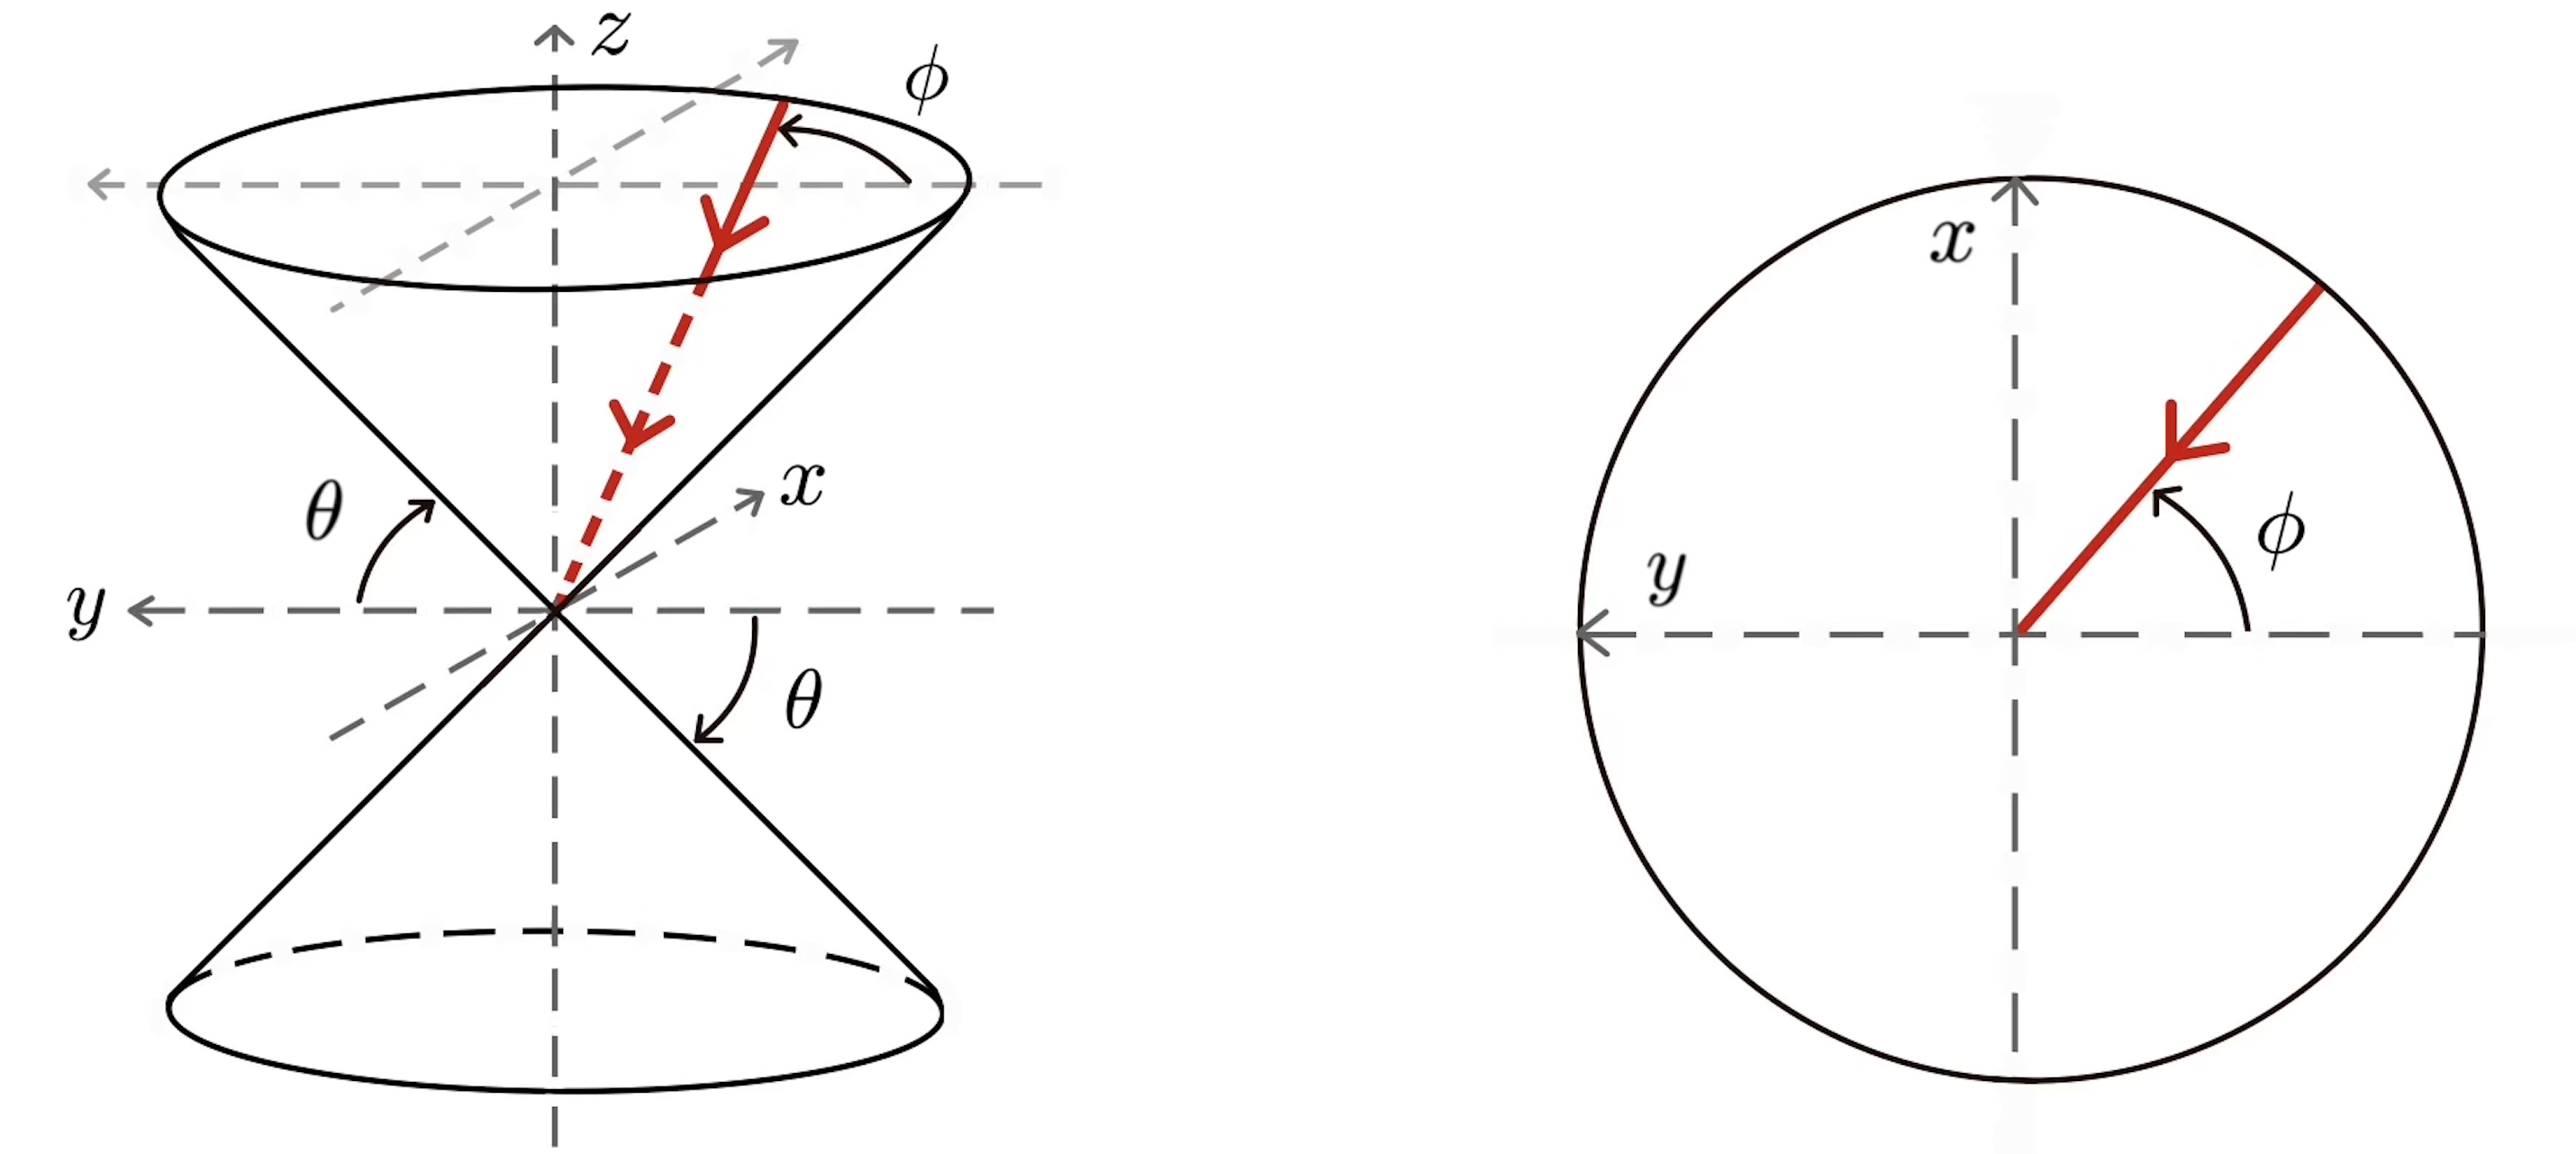
\includegraphics[scale=0.18, center]{Images/3d reflection.png}
  \caption{(a) A double cone that illustrates all probable rays propagating with frequency $\omega = \pm N \sin \theta$. Such a ray can be characterised by it's horizontal angle, $\phi$ which is drawn in red. (b) Top view of the cone. Based on Pillet \emph{et al.} (\protect\hyperlink{ref 37}{2019}).}
  \label{fig:13}
\end{figure} 

Moreover, the velocity vector, $\mathbf{u} = (u, v, w)$, for these waves follows the same trajectory i.e. it is parallel to the rays. Hence, the velocity vector also lies on this double cone. By considering the geometry of the double cone, it can be deduced that,
\begin{align*}
w = \pm \tan \theta \sqrt{u^2 + v^2}.
\end{align*}
In the 2D case, the propagation of internal waves were described by the velocity components and the angle of energy propagation, $\theta$. In the 3D case, the propagation of internal rays can be described by an additional component; the horizontal angle, $\phi$ (Pillet \emph{et al.} \hyperlink{ref 37}{2019}). It is this additional angle that invokes a lot of the complexity of the 3D model. 

\subsection{Reflection of 3D Internal Waves}
Now the geometry for the propagation of internal waves in 3D has been established, consider the reflection of these waves off an inclined plane. Consider a plane that is inclined at $\alpha$ with respect to the horizontal y-direction as depicted in Figure \ref{fig:14}. Such domains are of geological interest when studying river beds and estuaries. Denote $()_i$ and $()_r$ as incident and reflective wave properties respectively. 

\begin{figure}[h!]
  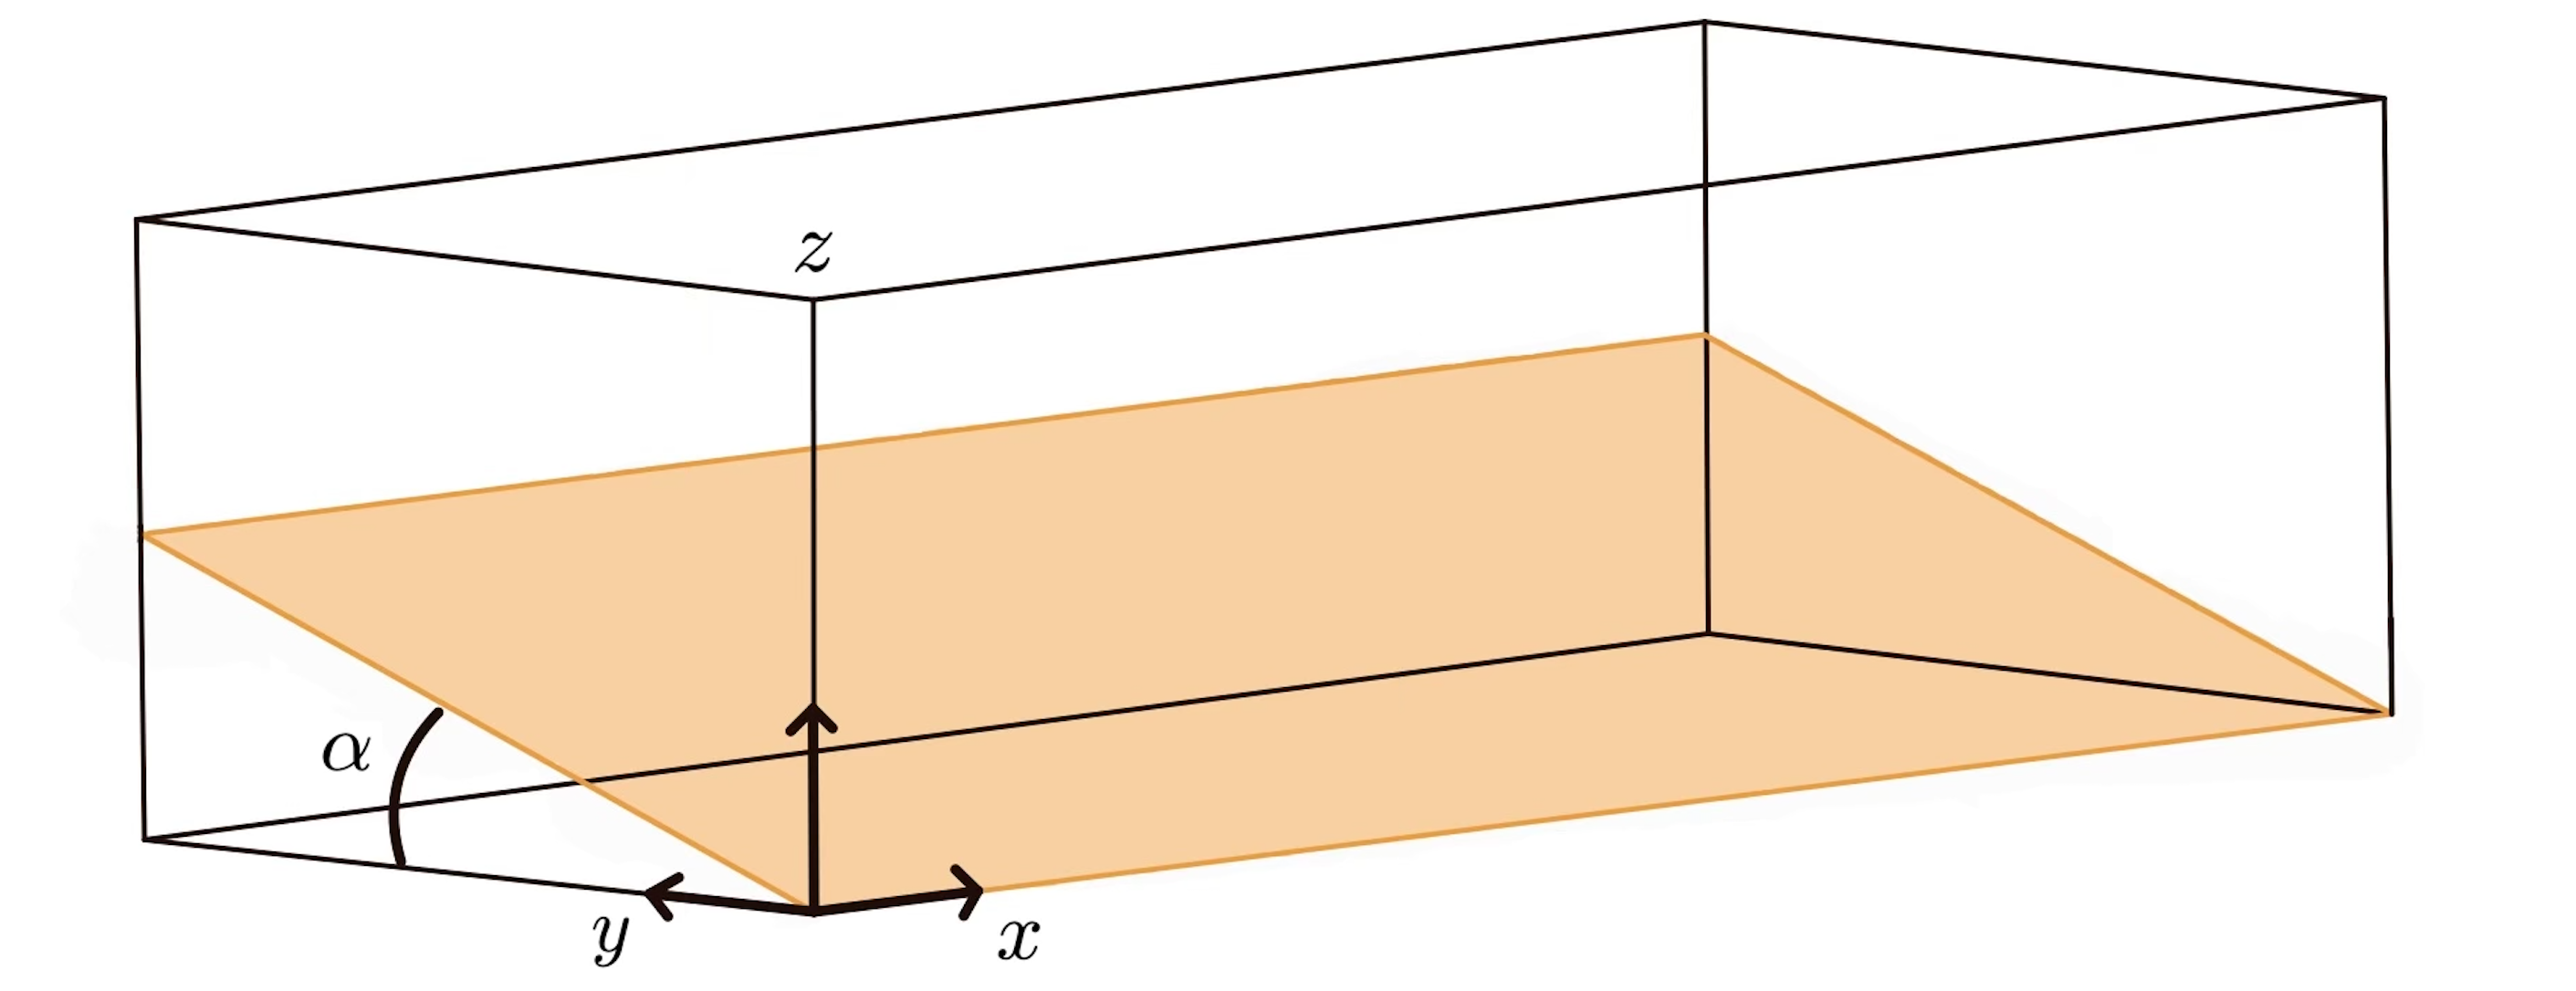
\includegraphics[scale=0.16, center]{Images/3d domain.png}
  \caption{3D trapezoidal domain. The orange rectangle illustrates the slope, inclined at an angle $\alpha$ with respect to the horizontal $(x,y)$ plane. Based on Pillet \emph{et al.} (\protect\hyperlink{ref 37}{2019}).}
  \label{fig:14}
\end{figure} 

The boundary conditions for this set up are as follows:
\begin{enumerate}
\item $u_r = u_i$ : the x-component of the velocity remains unchanged upon reflection. This conservation arises as a result of the invariance along the x-direction and inviscid nature.
\item $\theta_r = \pm\theta_i\mod \pi$ : the incident and reflected wave both remain on the double cone.
\item $w_r\cos\alpha - v_r\sin\alpha = - w_i\cos\alpha + v_i\sin\alpha$: the velocity normal component to the slope will change its sign upon reflection.
\end{enumerate}
Following convention similar to the 2D case, perform a rescaling so that rays propagate at $\theta = 45^{\circ}$. Define the velocity vector,
\begin{align}\label{eq:7.1}
(u, v, w) = (w\sin\phi, -w\cos \phi, w),
\end{align}
where $\phi$ denotes the horizontal angle of propagation with respect to the downslope directed y-axis as depicted in Figure \ref{fig:13}. Thus, $w^2_i = u^2_i + v^2_i$ and $w^2_r = u^2_r + v^2_r$. Noting condition (1), one may subtract these two equations from each other to obtain, 
\begin{align}\label{eq:7.2}
(w_r - w_i)(w_r + w_i) = (v_r - v_i)(v_r + v_i).
\end{align}
Now, condition (3) may be simplified by noting that the slope, $s$, can be defined as $s = \frac{\tan \alpha}{\tan\theta}$ where the normalisation is $\tan\theta$ (in this geometry this equals one). Condition (3) reduces to, 
\begin{align*}
w_i + w_r = s(v_i + v_r).
\end{align*}
Thus, by noting that the summation of the horizontal y-velocity between incident and reflected wave is nonzero, one substitutes this equation into equation \eqref{eq:7.2} to give,
\begin{align*}
w_r + w_i = s(v_r + v_i), ~~~~ v_r - v_i = s(w_r - w_i).
\end{align*}
Once the properties of the incident wave are known, one can establish those of the reflected wave,
\begin{align*}
u_r = u_i, ~~~~~~
v_r = \frac{(1+s^2)v_i - 2sw_i}{1- s^2},~~~~~~
w_r = \frac{-(1+s^2)w_i + 2sv_i}{1- s^2}.
\end{align*}
A quantity of interest is the law between reflected and incident horizontal angles, $\phi_r$ and $\phi_i$. Recall equation \eqref{eq:7.1}, one finds the relation, 
\begin{align}\label{eq:7.3}
\frac{u_r}{w_r} = \sin \phi_r = \frac{(s^2 - 1)\sin\phi_i}{1 + s^2 + 2s\cos \phi_i}.
\end{align}
This relation was first derived solely for a single reflection by Phillips (\hyperlink{ref 38}{1963}). Maas (\hyperlink{ref 39}{2005}) extended this theory and applied it iteratively. It is this law of reflection that gives rise to a whole class of behaviour that is absent in 2D. Indeed, the reflected angle, $\phi_r$, will vary as a result of different reflections. Although it may seem appropriate to study this angle, instead, one studies $\phi'_i$; the incident angle when the propagating ray returns towards the slope as illustrated in Figure \ref{fig:15}. 
\begin{figure}[h!]
  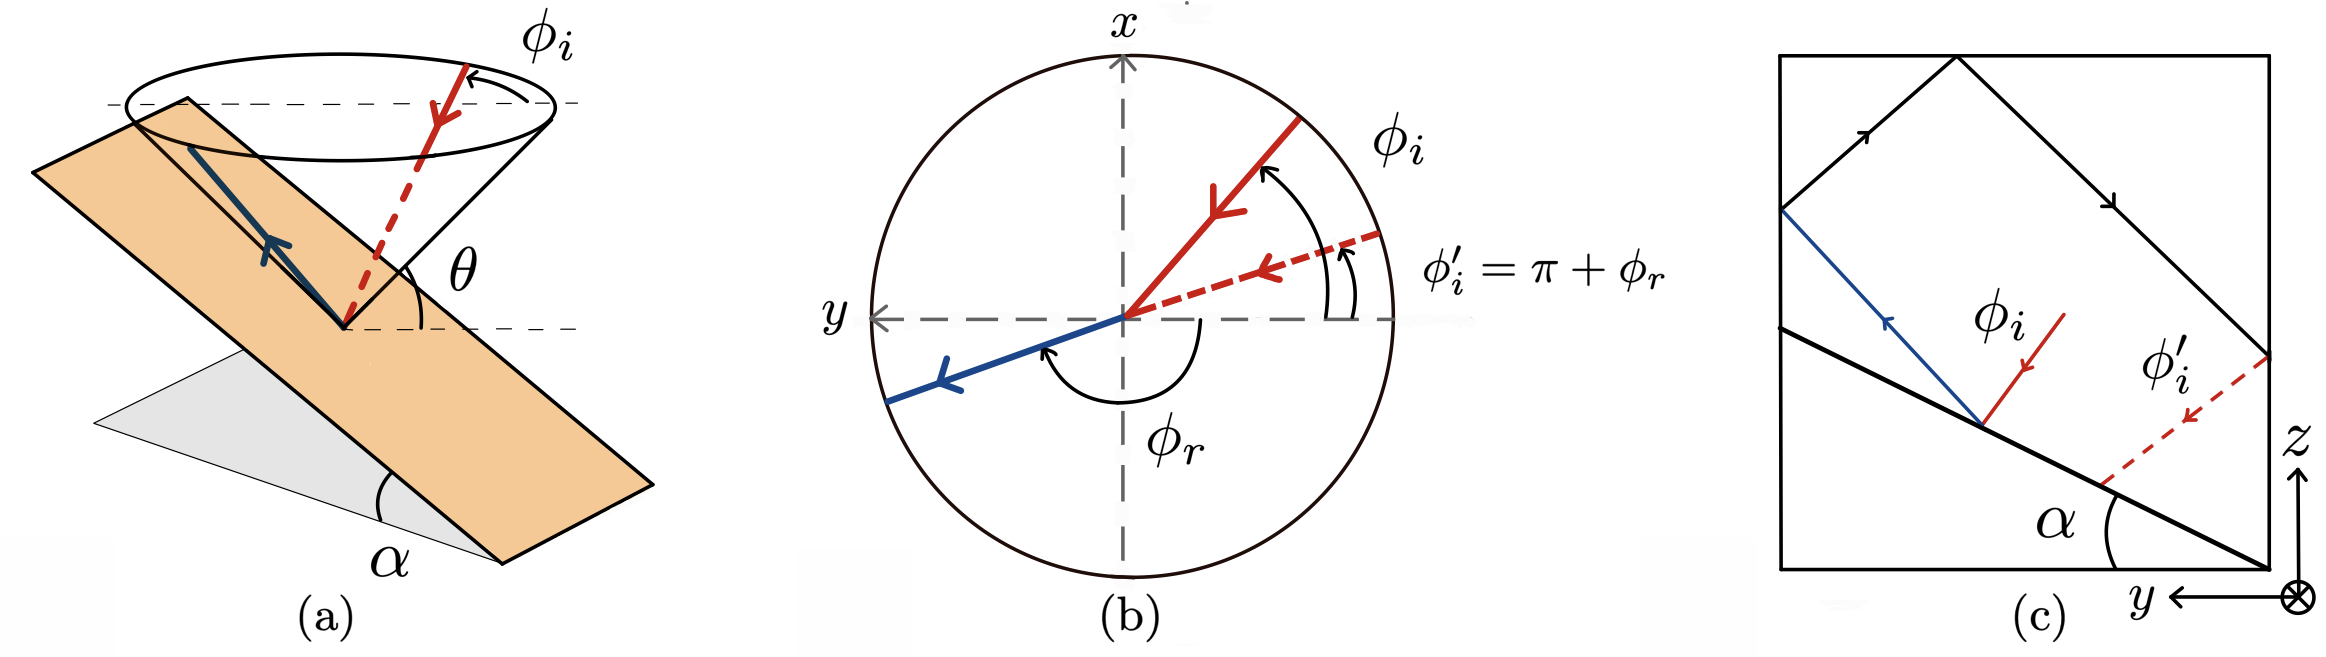
\includegraphics[scale=0.185, center]{Images/3 diag}
  \caption{Reflection of an internal wave beam off a subcritical, $s < 1$, inclined slope at angle $\alpha$ with respect to the horizontal $(x,y)$ plane. (a) Full view, (b) top view, and (c) $(y, z)$ plane. Initial trajectory of incident ray depicted in red and reflected ray depicted in blue. Dashed red ray illustrates $\phi'_i$ in (b) and (c). Based on Pillet \emph{et al.} (\protect\hyperlink{ref 37}{2019}).}
  \label{fig:15}
\end{figure} \\
Although Figure \ref{fig:15}(b) appears to suggest that $\phi'_i = \phi_r + \pi$, it is worth noting that this is not always the case, particularly when considering closed domains with horizontal and vertical boundaries. It is also possible for $\phi'_i = -\phi_r$; the reflected ray can reflect successively off a vertical and then horizontal wall before returning to the slope.

\subsubsection{Subcritical Reflections: $s < 1$}
To be consistent with numerical simulations (Pillet \emph{et al.} \hyperlink{ref 37}{2019}), consider the subcritical case where $s = \tan\alpha < 1$. First, it is important to note that for this case, the only area of physical interest is the top cone as the slope covers the lower cone. Then, one can deduce from \eqref{eq:7.3} that,
\begin{align*}
\phi_r = f(\phi_i, s) \equiv \sin^{-1} \bigg( \frac{(1-s^2)\sin\phi_i}{1 + s^2 + 2s\cos\phi_i} \bigg).
\end{align*}
Continuity must be achieved for $\phi'$ as it passes through $\pm \pi/2$ and so, one considers,
\begin{align*}
\psi(s) = \pi - f\big(\frac{\pi}{2}, s\big) = \pi - \sin^{-1}\bigg(\frac{(1- s^2)\sin(\frac{\pi}{2})}{1+s^2 + 2s\cos(\frac{\pi}{2})}\bigg) = \pi - \sin^{-1}\bigg(\frac{1- s^2}{1+s^2}\bigg).
\end{align*}
As a result, the following solution for $\phi'_i$ is obtained,
\begin{equation*}
\phi'_i = \left\{
        \begin{array}{ll}
            \pi - f(\phi_i, s), & \quad \phi_i < -\psi(s), \\
            f(\phi_i, s), & \quad  |\phi_i| < \psi(s), \\
            \pi + f(\phi_i, s), & \quad  \phi_i > -\psi(s). \\
        \end{array}
    \right.
\end{equation*}
\begin{figure}[h!]
  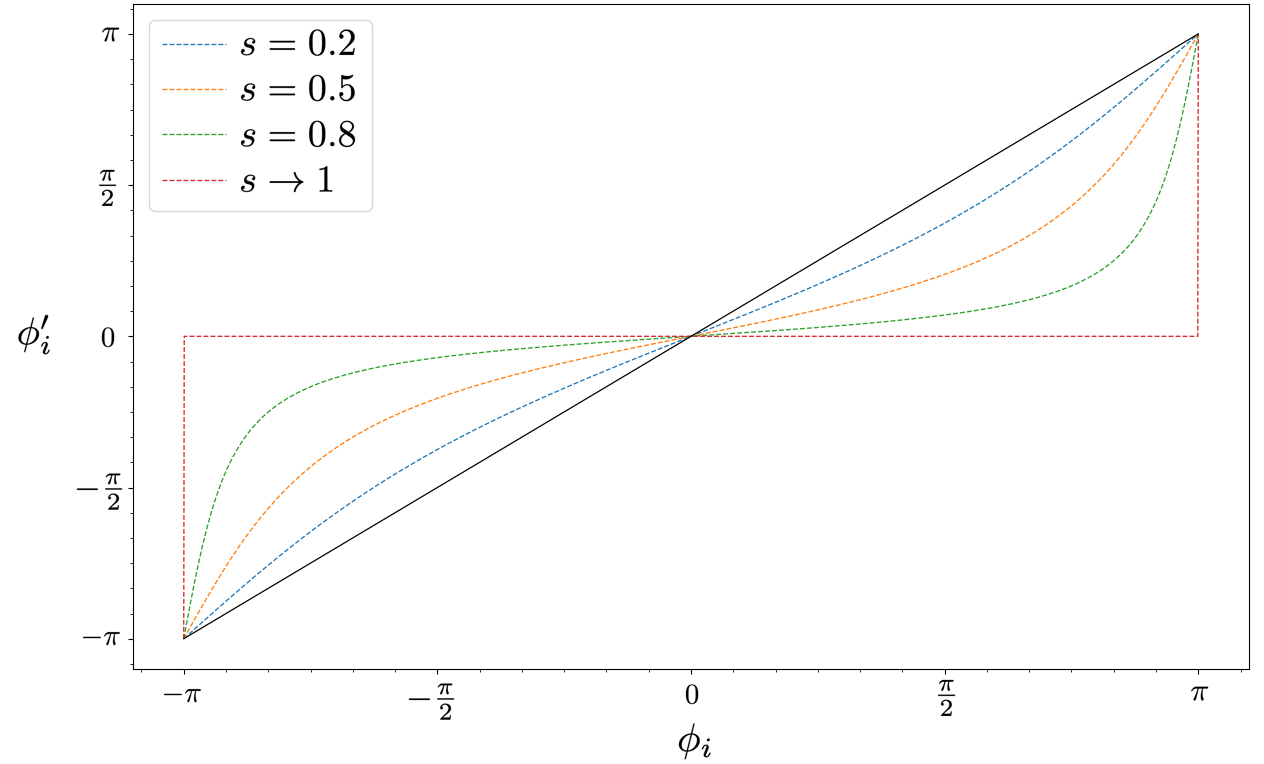
\includegraphics[scale=0.3, center]{Images/trapping plot.png}
  \caption{The function $\phi'_i$ for $\phi_i \in [-\pi, \pi]$ for four values of $s$ for which $s < 1$. The solid black line illustrates $\phi_i' = \phi_i$.}
  \label{fig:16}
\end{figure} \\
It is clear from Figure \ref{fig:16} that the relationship between $\phi'_i$ and $\phi_i$ varies according to the slope of the inclined plane, $s$, as expected. However, it is clear to see that, regardless of $s$ value, the graphs intersect at three distinct points, $\phi_i = 0$ and $\phi_i = \pm \pi$. Evaluating the derivative of $\phi'_i$,
\begin{align*}
\frac{d\phi'_i}{d\phi_i} = \frac{(1-s^2)\big(2s\sin^2(\phi_i) + \cos(\phi_i)(1 + s^2 + 2s\cos(\phi_i))\big)}{\big(1 + s^2 + 2s\cos(\phi_i)\big)\sqrt{(1 + s^2 + 2s\cos(\phi_i))^2 - \sin^2(\phi_i)(1 - s^2)^2}}.
\end{align*}
Evaluating at $\phi_i = 0, ~\pm \pi$ and and taking $s < 1$, it follows, 
\begin{align*}
\begin{split}
\text{At}&~~ \phi_i = 0, ~~~~~~ \frac{d\phi'_i}{d\phi_i} < 1, ~~~ \implies \text{stable fixed point},\\
\text{At}&~~ \phi_i = \pm \pi, ~~~ \frac{d\phi'_i}{d\phi_i} > 1, ~~~ \implies \text{unstable fixed point}.
\end{split}
\end{align*}
Thus, $\phi_i = 0$ is a stable fixed point which illustrates upslope propagation. Physically, this corresponds to the horizontal angle systematically reducing its horizontal angle. Moreover, a fascinating phenomenon known as the $trapping$ $effect$ has been established; the effect of the inclined slope results in the reflection of the internal wave ray reducing its horizontal angle. As depicted in Figure \ref{fig:16}, it is clear that as $s \rightarrow 1$, the trapping effect occurs faster. 

\subsubsection{Trapping vs Focusing}
As already established in Section (\hyperref[sec:2]{2}), the phenomenon of focusing involves a reduction in the reflected internal wave beam by a factor of $\gamma$. More simply, the distance between two parallel incident waves decreases upon reflection. However, the trapping effect describes the horizontal angle $\phi$ aligning with respect to the downslope direction of the inclined slope. 

Focusing can be extended to 3D geometries by considering the angle between two internal wave rays instead of the distance, that is, considering $\phi_2 - \phi_1$. Consider $\phi'_i$ as in Figure \ref{fig:16} and observe two initial internal wave rays as depicted in Figure \ref{fig:17}.
\begin{figure}[h!]
\centering
\begin{subfigure}[t]{.5\textwidth}
  \centering
  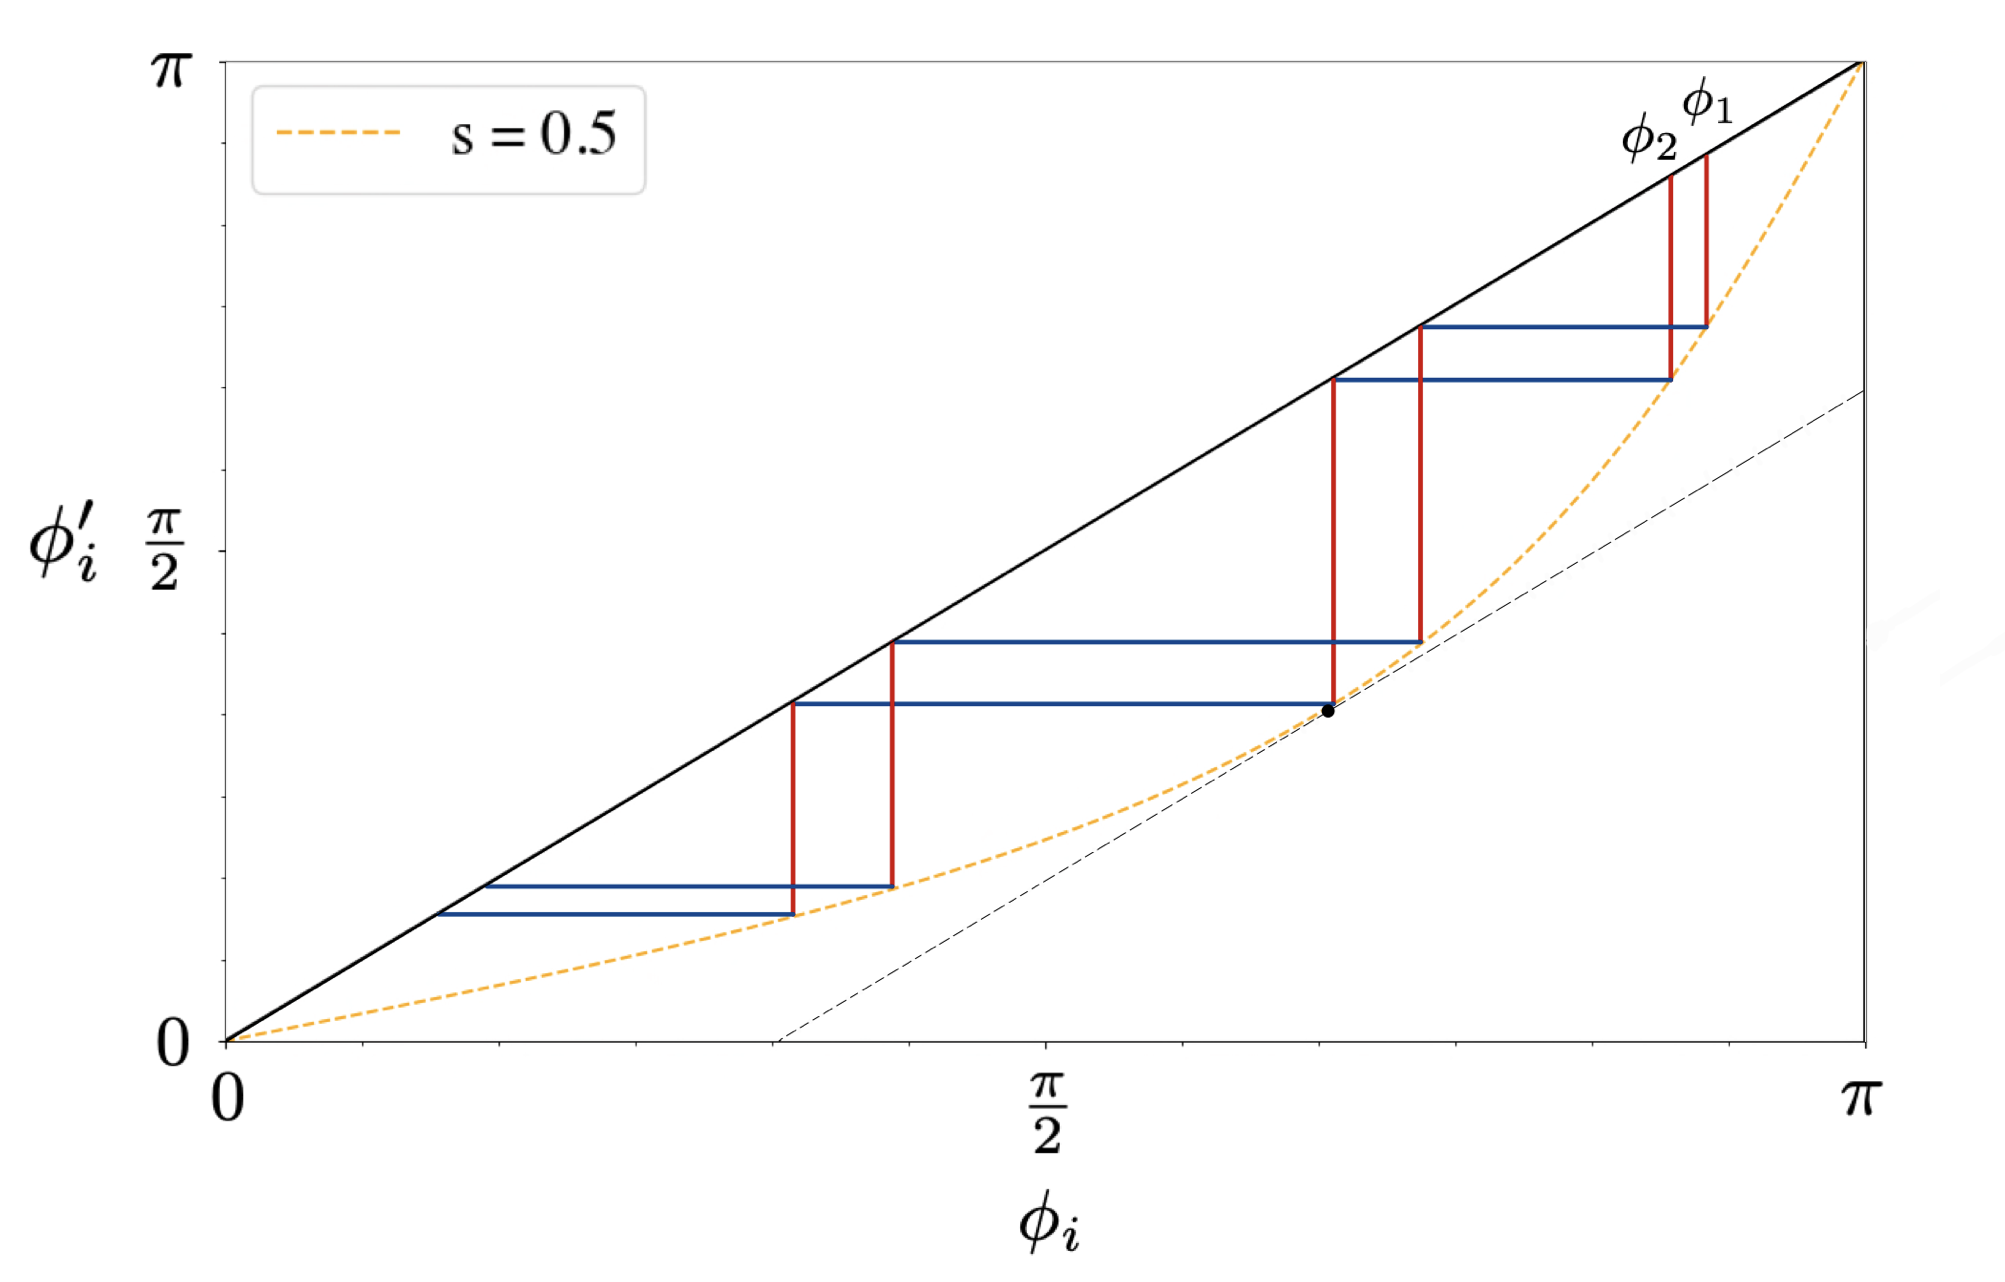
\includegraphics[width=1\linewidth]{Images/foc vs trap 2.PNG}
  \caption{$s = 0.5.$}
  \label{fig:sub1}
\end{subfigure}%
\begin{subfigure}[t]{.48\textwidth}
  \centering
  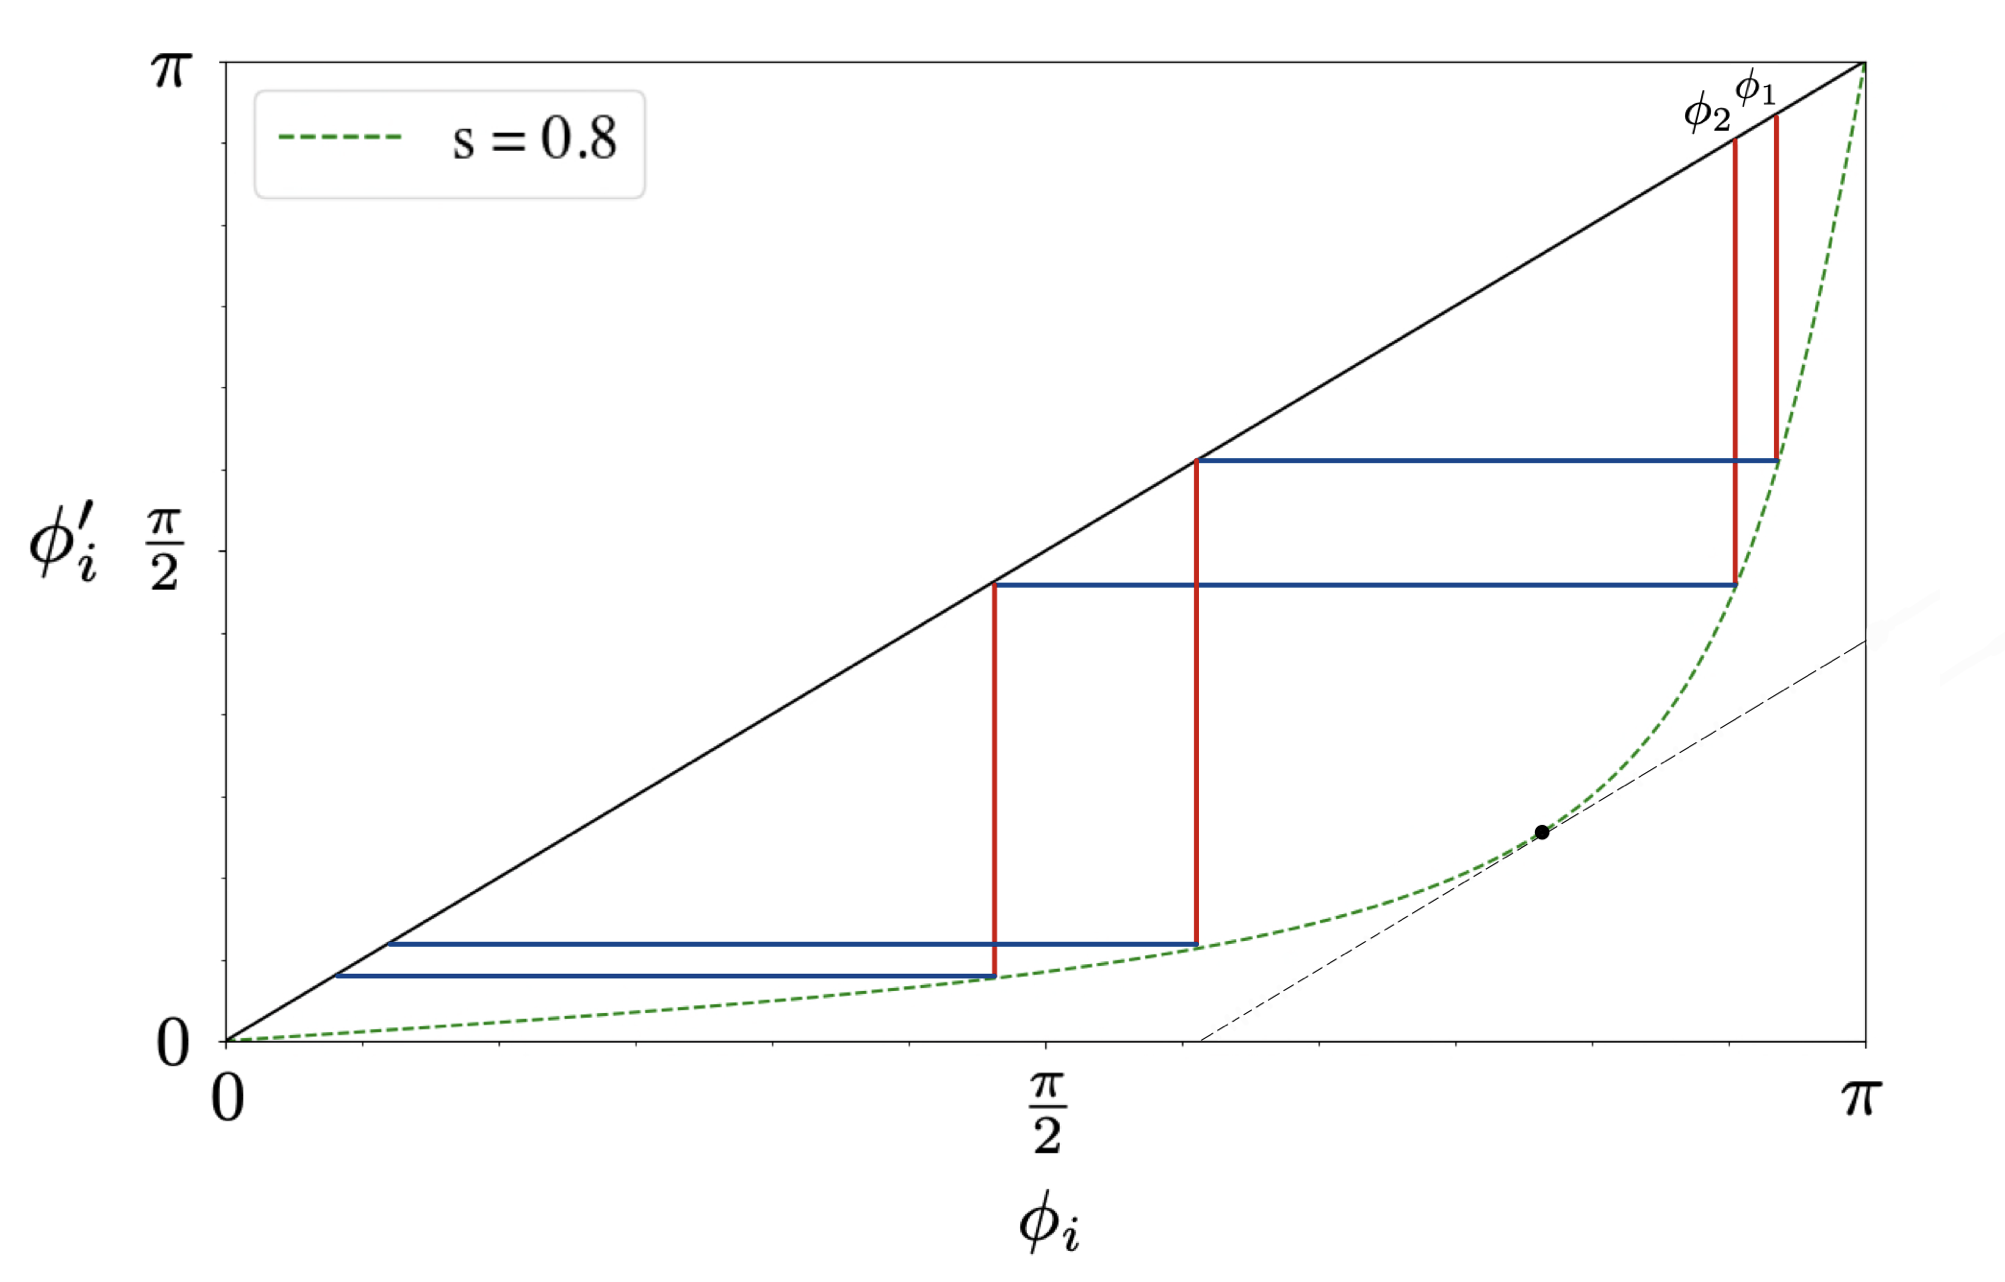
\includegraphics[width=1.05\linewidth]{Images/foc vs trap 1.PNG}
  \caption{$s = 0.8.$}
  \label{fig:a}
\end{subfigure}
\caption{The function $\phi'_i$ for $\phi_i \in [0, \pi]$ for two separate values of $s$ for which $s < 1$. Two different reflections with initial horizontal angles $\phi_1$ and $\phi_2$ are followed. Red lines correspond to incident rays and blue lines correspond to reflected rays. The solid black line illustrates $\phi_i' = \phi_i$. }
\label{fig:17}
\end{figure}

By exploring two different values of $s$, one can observe a relation between focusing and defocusing of the internal wave rays. Clearly, in both Figure \ref{fig:17}(a) and (b), two wave rays initially at some angular gap apart can become defocused (angular gap increases) and then focused (angular gap decreases) again. Figure \ref{fig:17}(a) illustrates two initial defocusing reflections followed by one focusing reflection. Figure \ref{fig:17}(b) depicts one defocusing reflection followed by a focusing reflection. However, in both cases, the angle of each internal wave ray decreases and hence, trapping occurs. 

Both Figure \ref{fig:17}(a) and (b) depict the critical point between focusing and defocusing reflections as seen by the black circle where the black dashed line with slope $1$ intersects the graph. Clearly, for any reflections above this critical point, defocusing occurs and below the critical point, focusing occurs. More specifically, 
\begin{align*}
\text{Defocusing:} ~~~ \iff \left.\frac{d\phi'_i}{d\phi_i}\right|_{\phi} > 1, ~~~~~ \text{for}~~ \phi \in [\phi_1, \phi_2], \\
\text{Focusing:} ~~~~~~ \iff \left.\frac{d\phi'_i}{d\phi_i}\right|_{\phi} < 1, ~~~~~ \text{for}~~ \phi \in [\phi_1, \phi_2].
\end{align*}
Thus, the notions of focusing and trapping describe different phenomenon and are not always analogous to each other. 

\subsection{Wave Attractors in Three-Dimensions}
Now the theory behind the trapping effect has been established, one can consider the formation of IWAs in such a geometry. Results stated in this section were simulated numerically by Pillet \emph{et al.} (\hyperlink{ref 37}{2019}) and are stated in this section for illustrative purposes. 

The true power behind the trapping effect is demonstrated in this geometry; after successive reflections on a subcritical slope, $\phi$ will converge to the fixed point $\phi = 0$ as illustrated in Figure \ref{fig:16}. Hence, any given ray will eventually converge to the $(y, z)$ plane resulting in the trapping of internal waves. One therefore expects similar IWAs to be observed in the 3D case. 

\subsubsection{The (1,1) Attractor}
Noting that $(1,1)$ attractors can have $\phi'_i = \pi + \phi_r$ as depicted in Figure \ref{fig:15}(b), then this setup will facilitate trapping. Parameters were chosen to be consistent with propagation along the double cone and the production of a $(1,1)$ attractor as depicted in Figure \ref{fig:18}. Moreover, they were also chosen such that trapping occurs but not too fast or too slow so that the correct analysis can be made.
\begin{figure}[h!]
  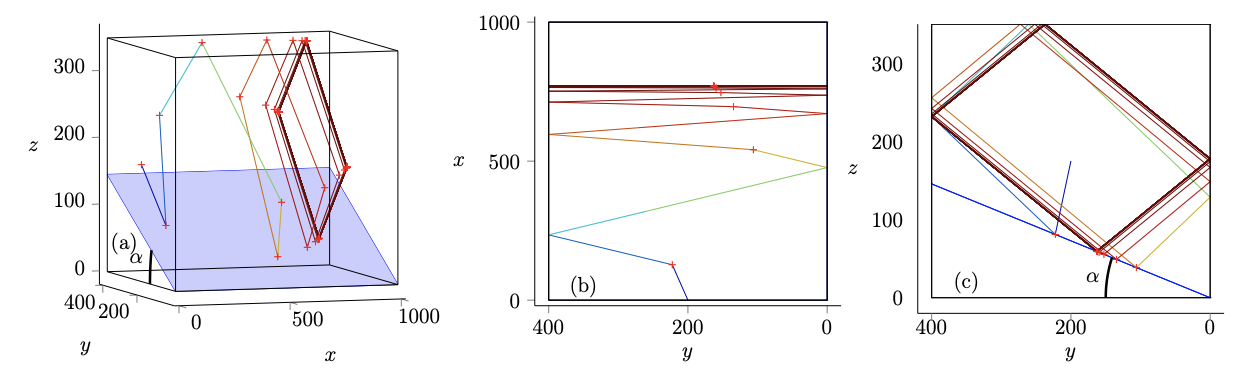
\includegraphics[scale=0.6, center]{Images/trapping_effect}
  \caption{The trajectory of one internal wave beam propagating in the domain depicted in Figure \ref{fig:14} filled with a linearly stratified fluid. Parameters: $H = 350$, $W = 400$, $L=1000$, $\alpha = 20^{\circ}$, $\theta = 35^{\circ}$. The beam is directed in the negative z-direction from the position, $x_0 = 0$, $y_0 = W/2$, $\phi_0 \approx \pi/2$. (a) The behaviour of the full domain with red crosses depicting rebounds on the slope and side walls. (b) The convergence $\phi_i \rightarrow 0$ with the red crosses highlighting the rebounds only on the slope. (c) The limit cycle of the $(1,1)$ attractor. Moreover, the colour of the ray increases from blue to red as the ray continues to reflect. Pillet \emph{et al.} (\protect\hyperlink{ref 37}{2019}).}
  \label{fig:18}
\end{figure} \\
Here, an internal wave ray launched initially in the x-direction will eventually evolve, after successive reflections on the inclined slope, onto an internal wave attractor purely in the $(y, z)$ plane. This wave attractor is identical to those obtained in 2D as seen in Figure \ref{fig:5}(b) (Maas \& Lam \hyperlink{ref 17}{1995}; Maas \& Lam \hyperlink{ref 10}{2005}; Brouzet \emph{et al.} \hyperlink{ref 26}{2016}).

In contrast to 2D, the propagation of the rays depend on the additional angle, $\phi$. In this case, $\phi = 0$, in the asymptotic limit which illustrates trapping. It is clear to see the effect of trapping in 3D; an initial propagation in the x-direction leads to the formation of an attractor in the $(y, z)$ plane.
\subsubsection{Attracting Two-Dimensional Manifold}
One important quantity worth measuring is the final position of the IWA and considering whether this quantity remains the same regardless of starting position. Denote this quantity $x_\infty$; it describes the longitudinal coordinate of the trapping $(y, z)$ plane. 

The left image in Figure \ref{fig:19} demonstrates the varying $x_\infty$ for different initial conditions; the initial $y$ and $z$ values are varied as denoted by the stars in figure \ref{fig:19} and their corresponding converged IWAs are depicted. In the right image, the initial horizontal angle, $\phi$ is varied and the corresponding converged IWAs are also shown. From the two figures, one can deduce that the value of $x_\infty$ varies only slightly for a variation in $(y,z)$ but strongly for $\phi$ values. The collection of attractors seen in both figures, is a phenomenon known as an \emph{attracting two dimensional manifold}. 
\begin{figure}[h!]
  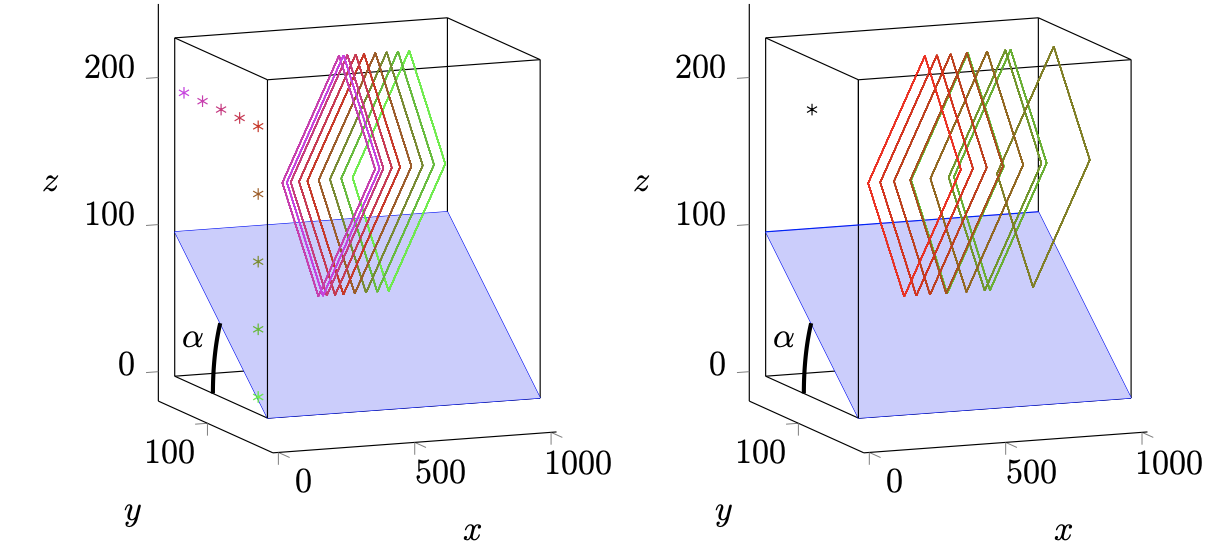
\includegraphics[scale=0.5, center]{Images/manifold}
  \caption{The steady paths of the $(1,1)$ attractor shown for various launching methods. The left-hand varies the launching positions in the $x = 0$ plane with $\phi_0 = \pi/2$. The initial position and attractor are depicted by the same colour. The right-hand keeps the initial launching position fixed (black star) but changes the value of $\phi_0$ between $20^{\circ}$ (grey) and $90^{\circ}$ (red). Pillet \emph{et al.} (\protect\hyperlink{ref 37}{2019}).}
  \label{fig:19}
\end{figure} \\
This result implies that the initial starting point or horizontal angle do not have an influence a change in the attractor; regardless of starting position one eventually gets the same attractor, only its position $x_\infty$ changes. Interestingly, once a wave attractor is known to exist in 2D, its 3D generalisation will guarantee trapping of the rays during their propagation.

% -----------------------------------------------------------------------------
% -----------------------        Conclusion        --------------------------
% -----------------------------------------------------------------------------
\section{Conclusion}
The main objectives of this essay were to provide a review of IWAs and to understand their properties in different regimes. Firstly, the behaviour of internal waves were established with particular emphasis on their energy propagation and reflective nature (LeBlond \& Mysak \hyperlink{ref 4}{1981}; Mowbray \& Rarity \hyperlink{ref 5}{1967}; Phillips \hyperlink{ref 7}{1966}). The governing yet ill-posed wave equation was then obtained (Swart \emph{et al.} \hyperlink{ref 15}{2007}). As a result, techniques such as ray tracing were used to overcome this technicality and solutions were found using fundamental intervals and the travelling wave solution (Lam \& Maas  \hyperlink{ref 18}{2008}). Using the reflective property of internal waves, energy initially injected into the domain was shown to concentrate around the IWA.

Of course, in real world processes, an infinite of energy is unphysical and so, viscous effects take hold. Initially, viscous decay along an internal wave beam was derived and showed that higher wavenumbers decay more rapidly (Thomas \& Stevenson \hyperlink{ref 21}{1972}; Tabaei \& Akylas \hyperlink{ref 22}{2003}). Indeed, viscosity was seen to play a role in controlling the wave branches so attention was drawn to the equilibrium thickness of such attractors. Scaling arguments were obtained for the existence of viscous dissipation at the shear layers, lateral and reflecting walls. Despite previous literature (Hazewinkel \emph{et al.} \hyperlink{ref 27}{2008}), it was shown that dissipation at the rigid walls were substantial and the thickness of the branches were not solely described by internal shear dissipation (Beckebanze \emph{et al.} \hyperlink{ref 8}{2017}).

Non-linear stratification was then considered. The exponential stratification illustrated wave beams that tended towards the horizontal with a focus of energy. Such a regime did not facilitate IWAs. However, considering a hyperbolic stratification (Hazewinkel \hyperlink{ref 24}{2010}), the wave attractor branches were curved at the point of strongest stratification. This contrasted to the $N = const.$ case where the wave rays were straight lines. Indeed, this stratification profile facilitated IWAs in the trapezoidal domain. Moreover, energy becomes focused around the IWA and so, when the energy is increased, one expects instabilities to occur. Attention was drawn towards the TRI and its presence in internal wave beams and IWAs (Craik \hyperlink{ref 32}{1988}). In particular, TRI was seen to act as a mechanism to balance geometric focusing. 

Finally, IWAs were extended to the 3D case where the dispersion relation for internal waves described rays propagating on a double cone. Conditions for the reflection of internal waves in a 3D trapezoidal domain were then illustrated. This section featured subcritical reflections to be consistent with the literature (Pillet \emph{et al.} \hyperlink{ref 37}{2019}) and in doing so, the phenomenon of trapping was established. Anti-parallels were then drawn between trapping and focusing. A final comment was made on attracting 2D manifolds and in particular, the robustness of IWAs in the 3D domain. 

Although the area of IWAs has been extensively studied, many questions remain open. Domains studied in this essay are limited when considering real world systems. Guo and Holmes-Cerfon (\hyperlink{ref 42}{2016}) explored attractors in oceanography but much more extensive research is needed to truly understand WAs in geophysical and astrophysical systems. They found that WAs are likely to exist with a non-negligible probability of 10 attractors per 1000km. However, they concluded that more complex attractors are more likely to be present. For this reason, future work will need to explore the effects of non-linearities and energy cascade in more complicated attractors. 

Substantial research on WAs in the ocean considered a bi-dimensional set up (Guo and Holmes-Cerfon \hyperlink{ref 42}{2016}; Echeverri \emph{et al.} \hyperlink{ref 43}{2011}). Exploring attractors in 3D is therefore a vital and active area of current research. Indeed, observations were found for the 3D trapezoidal domain (Pillet \emph{et al.} \hyperlink{ref 37}{2019}) but further research is required to understand IWAs in more complex domains. Moreover, Earth's rotation also plays an important role and so inertio-gravity waves are present. These waves aren't expected to modify the linear processes governing the wave attractors but it will vastly affect the TRI. Therefore, researching gravito-inertial waves will be important in future research. 

To this day, understanding internal wave attractors in physical systems remains an active area of research within applied mathematics. It plays a pivotal role in establishing waves seen in geophysical and astrophysical systems. The results presented in this essay covers an area of applied mathematics that is, and will always remain, a fundamental interest to mathematicians and physicists.

% -----------------------------------------------------------------------------
% -----------------------        References        --------------------------
% -----------------------------------------------------------------------------
% Note, these references were written manually but you can use alternative LaTeX reference packages to make it easier!
\section{References}
\hypertarget{ref 16}{\makebox[\linewidth][s]{\textsc{Bajars, J. Frank, J. \& Maas, L. R. M.} 2012 On the appearance of internal wave attractors due} \\\hspace*{1.1cm} to an initial or parametrically excited disturbance. \emph{J. Fluid Mech.} \textbf{714}, 283-311.}\\
\hypertarget{ref 29}{\makebox[\linewidth][s]{\textsc{Beckebanze, F. Keady, G.} 2016 On functional equations leading to exact solutions for standing} \\\hspace*{1.1cm} internal waves. \emph{Wave Motion.} \textbf{60}, 181-195.}\\
\hypertarget{ref 8}{\makebox[\linewidth][s]{\textsc{Beckebanze, F. Brouzet, C. Sibgatullin, I. N. \& Maas, L. R. M.} 2018 Damping of quasi- }\\\hspace*{1.17cm} two dimensional internal wave attractors by rigid wall friction. \emph{J. Fluid Mech.} \textbf{841}, 614-635.} \\
\hypertarget{ref 33}{\makebox[\linewidth][s]{\textsc{Bourget, B. Dauxious, T. Joubard, S. \& Odier, P.} 2013 Experimental study of parametric} \\\hspace*{1.1cm} subharmonic instability for internal place waves. \emph{J. Fluid Mech.} \textbf{723}, 1-20.}\\
\hypertarget{ref 26}{\makebox[\linewidth][s]{\textsc{Brouzet, C. Sibgatullin, I. N. Scolan, H. Ermanyuk E. V. \& Dauxious, T.} 2016 Internal} \\\hspace*{1.1cm} wave attractors examined using laboratory experiments and 3D numerical simulations. \\\hspace*{1.1cm} \emph{J. Fluid Mech.} \textbf{793}, 109-131.}\\
\hypertarget{ref 9}{\makebox[\linewidth][s]{\textsc{Brouzet, C.} 2016 Internal wave attractors: from geometric focusing to non-linear energy cascade} \\\hspace*{1.1cm} and mixing. \emph{Fluid Dyn.}, HAL, University of Lyon.}\\
\hypertarget{ref 32}{\makebox[\linewidth][s]{\textsc{Craik, A. D. D.} 1988 \emph{Wave interactions and fluid flows.} Cambridge University Press, Cambridge.}}\\
\hypertarget{ref 43}{\makebox[\linewidth][s]{\textsc{Echeverri, P. Yokossi, T. Balmforth, N. J. \& Peacock, T.} 2011 Tidally generated internal} \\\hspace*{1.1cm} wave attractors between double ridges. \emph{J. Fluid Mech.} \textbf{669}, 354-374.}\\
\hypertarget{ref 6}{\makebox[\linewidth][s]{\textsc{Gostiaux, L. Didelle, H. Mercier, S. \& Dauxious, T.} 2007 A novel internal waves generator.} \\\hspace*{1.1cm}  \emph{Exp Fluids} \textbf{42}, 123-130.}\\
\hypertarget{ref 25}{\makebox[\linewidth][s]{\textsc{Grisouard, N. Staquet, C. \& Pairaud, I.} 2008 Numerical simulation of a two-dimensional} \\\hspace*{1.1cm} internal wave attractors. \emph{J. Fluid Mech.} \textbf{614}, 1-14.}\\
\hypertarget{ref 42}{\makebox[\linewidth][s]{\textsc{Guo, Y. \& Holmes-Cerfon, M.} 2016 Internal wave attractors over random, small amplitude topog-} \\\hspace*{1.1cm}raphy. \emph{J. Fluid Mech.} \textbf{787}, 148-174.}\\
\hypertarget{ref 34}{\makebox[\linewidth][s]{\textsc{Hasselmann, K.} 1962 On the non-linear energy transfer in a gravity-wave spectrum Part 1. Gen-} \\\hspace*{1.1cm}eral theory. \emph{J. Fluid Mech.} \textbf{12}, 481-500.}\\
\hypertarget{ref 27}{\makebox[\linewidth][s]{\textsc{Hazewinkel, J. Van Breevoort, P. Dalziel, S. B. \& Maas, L. R. M.} 2008 Observations on} \\\hspace*{1.1cm} the wavenumber spectrum and evolution of an internal wave attractor. \emph{J. Fluid Mech.} \\\hspace*{1.1cm} \textbf{598}, 373-382.}\\
\hypertarget{ref 24}{\textsc{Hazewinkel, J.} 2010 \emph{Attractors in stratified fluids.} Utrecht University.}\\
\hypertarget{ref 3}{\makebox[\linewidth][s]{\textsc{Kundu, P. K. Cohen, I. \& Dowling, D. R.} 2016 \emph{Fluid Mechanics, 6th Eds.} Academic Press,} \\\hspace*{1.1cm} Waltham.}\\
\hypertarget{ref 18}{\makebox[\linewidth][s]{\textsc{Lam, F-P. A. \& Maas, L. R. M.} 2008. Internal wave focusing revisited: A reanalysis and new} \\\hspace*{1.1cm} theoretical links. \emph{Fluid Dyn. Res.} \textbf{40}, 95-122.}\\
\hypertarget{ref 4}{\textsc{LeBlond, P. H. \& Mysak, L. A.} 1981 \emph{Waves in the Ocean} Elsevier.}\\
\hypertarget{ref 31}{\textsc{Lighthill, J.} 1978 \emph{Waves in Fluids.} Cambridge University Press, Cambridge.}\\
\hypertarget{ref 17}{\makebox[\linewidth][s]{\textsc{Maas, L. R. \& Lam, F. P. A.} 1995 Geometric focusing of internal waves. \emph{J. Fluid Mech.} \textbf{300}}, \\\hspace*{1.1cm} 1- 41.}\\
\hypertarget{ref 11}{\makebox[\linewidth][s]{\textsc{Maas, L. R. M. Benielli, D. Sommeria, J. \& Lam, F. P. A.} 1997 Observation of an internal} \\\hspace*{1.1cm} wave attractor in a confined stably stratified fluid. \emph{Nature} \textbf{388}, 557-561.}\\
\hypertarget{ref 39}{\makebox[\linewidth][s]{\textsc{Maas, L. R. M. } 2005 Wave attractors: linear yet nonlinear. \emph{Int. J. Bifurcat. Chaos} \textbf{15},(09)} \\\hspace*{1.1cm} 2757-2782.}\\
\hypertarget{ref 10}{\makebox[\linewidth][s]{\textsc{Maas, L. R. M. \& Lam, F. P. A. } 2005 Geometric focusing of internal waves. \emph{J. Fluid Mech.}} \\\hspace*{1.1cm} \textbf{300}, 1 - 41.}\\
\hypertarget{ref 20}{\makebox[\linewidth][s]{\textsc{Maas, L. R. M.} 2009 Exact analytic self-similar solution of a wave attractor field. \emph{Physica D.} \textbf{238},} \\\hspace*{1.1cm} 502-505.}\\
\hypertarget{ref 5}{\makebox[\linewidth][s]{\textsc{Mowbray, D. E. \& Rarity, S. H.} 1967 A theoretical and experimental investigation of the phase} \\\hspace*{1.1cm} configuration of internal waves of small amplitude in a density stratified liquid. \\\hspace*{1.1cm} \emph{J. Fluid Mech.} \textbf{28}, 1-16.} \\
\hypertarget{ref 14}{\makebox[\linewidth][s]{\textsc{Müller, P. \& Liu, X.} 2000 Scattering of internal waves at finite topography in two dimensions} \\\hspace*{1.1cm} part i: theory and case studies. \emph{J. Phys. Oceanogr} \textbf{30}, (3) 532-549.}\\
\hypertarget{ref 2}{\makebox[\linewidth][s]{\textsc{Ogilvie, G. \& Lin, D. N. C.} 2004 Tidal dissipation in rotating giant planets. \emph{Astrophys. J} \textbf{610}(1),} \\\hspace*{1.1cm} 477-509.}\\
\hypertarget{ref 13}{\makebox[\linewidth][s]{\textsc{Ogilvie, G. I.} 2005 Wave attractors and the asymptotic dissipation rate of tidal disturbances.}\\\hspace*{1.1cm}  \emph{J. Fluid Mech.} \textbf{543}, 19-44.}\\
\hypertarget{ref 1}{\textsc{Pedlosky, J.} 2003 \emph{Waves in the Ocean and Atmosphere}. Springer.}\\
\hypertarget{ref 38}{\makebox[\linewidth][s]{\textsc{Phillips, O. M.} 1963 Energy transfer in rotating fluids by reflection of inertial waves. \emph{Phys. Fluids} }\\\hspace*{1.1cm} \textbf{6}, 513-520.}\\
\hypertarget{ref 7}{\makebox[\linewidth][s]{\textsc{Phillips, O. M.} 1966 \emph{The dynamics of the upper ocean.} Cambridge University Press, Cambridge.}}\\
\hypertarget{ref 37}{\makebox[\linewidth][s]{\textsc{Pillet, G. Maas, L. R. M \& Dauxious, T.} 2019 Internal wave attractors in 3D geometries: A} \\\hspace*{1.1cm} dynamical systems approach. \emph{Europ. J. Mech.} \textbf{77}, 1-16.}\\
\hypertarget{ref 36}{\makebox[\linewidth][s]{\textsc{Rabatti, A. \& Maas, L. R. M.} 2014 Inertial wave rays in rotating spherical fluid domains. }\emph{J. \\\hspace*{1.1cm} Fluid Mech.} \textbf{758}, 621-654.}\\
\hypertarget{ref 12}{\textsc{Rieutord, M. Georgeot, B. \& Valdettaro, L.} 2001 Intertial waves in a rotating spherical \\\hspace*{1.1cm} shell: attractors and asymptotic spectrum. \emph{J. Fluid Mech.} \textbf{435}, 103 - 144}.\\
\hypertarget{ref 50}{\textsc{Roger, T.} 2002 \emph{Internal wave focusing in a non-uniform stratification}, ENSTA (Internship project \\\hspace*{1.1cm} with S.B. Dalziel at the University of Cambridge).}\\
\hypertarget{ref 28}{\textsc{Schlichting, H. \& Gersten, K.} 2000 \emph{Boundary-Layer Theory.} Springer.}\\
\hypertarget{ref 35}{\makebox[\linewidth][s]{\textsc{Scolan, H. Ermanyuk, E. \& Dauxious, T.} 2013 Nonlinear fate of internal wave attractors.} \\\hspace*{1.1cm} \emph{Physical Review Letters.} \textbf{110}, 234501.}\\
\hypertarget{ref 19}{\makebox[\linewidth][s]{\textsc{Sibgatullin, I. N. \& Ermanyuk, E. V.} 2019 Internal and inertial wave attractors: A review. }\\\hspace*{1.1cm} \emph{J. App. Mech. \& Tech. Phys.} \textbf{60}, 284-302.}\\
\hypertarget{ref 15}{\makebox[\linewidth][s]{\textsc{Swart, A. Sleijpen, G. L. Maas, L. R. M. \& Brandts, J.} 2007 Numerical solution of the}\\\hspace*{1.1cm} two-dimensional Poincaré equation. \emph{J. Comput. Appl. Math.} \textbf{200}, 317-341.}\\
\hypertarget{ref 22}{\makebox[\linewidth][s]{\textsc{Tabaei, A. \& Akylas, T.} 2003 Nonlinear internal gravity wave beams. \emph{J. Fluid Mech.} \textbf{482},} \\\hspace*{1.1cm} 141-161.}\\
\hypertarget{ref 21}{\makebox[\linewidth][s]{\textsc{Thomas, N. H. \& Stevenson, T. N.} 1972 A similarity solution for viscous internal waves.} \\\hspace*{1.1cm} \emph{J. Fluid Mech.} \textbf{54}, (3) 495-506.}\\
\hypertarget{ref 44}{\textsc{Traub, J. F.} 1964 Iterative methods for solutions of equations. Prentice-Hall, Englewood Cliffs, \\\hspace*{1.1cm} NJ.}\\
\hypertarget{ref 23}{\textsc{Voisin, B.} 2003 Limit states of internal wave beams. \emph{J. Fluid Mech.} \textbf{496} 243-293.}\\
\end{document}


